%--- Kapitel 5
\cleardoublepage
\chapter{Prozessmodellierung mit Petrinetzen}
\label{sec:Kap-5}

%--- Kapitel 5.1 - 5.12
% \clearpage Hier keinen Seitenumbruch!
\section[Vorlesung 1: Modellierung von (dynamischen) Systemen und\\ Prozessen]{Vorlesung 1: Modellierung von (dynamischen) Systemen und Prozessen}
\markright{Vorlesung 1: Modellierung von (dynamischen) Systemen und Prozessen}

\subsection*{Grundlegende Elemente der Verhaltensmodellierung}

Eine Modellierungssprache legt fest, 
\marginline{Syntax und Semantik der Modellierungs\-sprache}
welche Elemente zur Beschreibung eines Originals genutzt und wie sie dargestellt werden. Ähnlich wie in einer natürlichen Sprache gibt es dabei eine Syntax: Formale Regeln bestimmen, welche Symbole zur Darstellung der verschiedenen Elemente verwendet werden und wie sie kombiniert werden können. Die Semantik hingegen definiert die Bedeutungen dieser Symbole. Sie bestimmt also, \textbf{wie} Originale abgebildet werden und damit auch, welche ihrer Aspekte durch die jeweilige Modellierungssprache hervorgehoben werden. Ein Element kann in verschiedenen Modellierungssprachen unterschiedlich benannt und durch unterschiedliche Symbole repräsentiert werden \cite{ros12}.

Unterschiede ergeben sich aus dem jeweiligen Modellierungskontext und -zweck. Die Abbildungen \ref{fig:grundelemente_EPK} und \ref{fig:grundelemente_BPMN} zeigen als Beispiele die zwei heute gängigen Prozess\-model\-lie\-rungs\-sprachen EPK und BPMN (im Vorlesungsvideo werden weitere Sprachen vorgestellt).

\begin{figure}[t]
	\begin{addmargin*}[0cm]{-\marginparwidth}
	\begin{addmargin*}[0cm]{-\marginparsep}
		\centering
		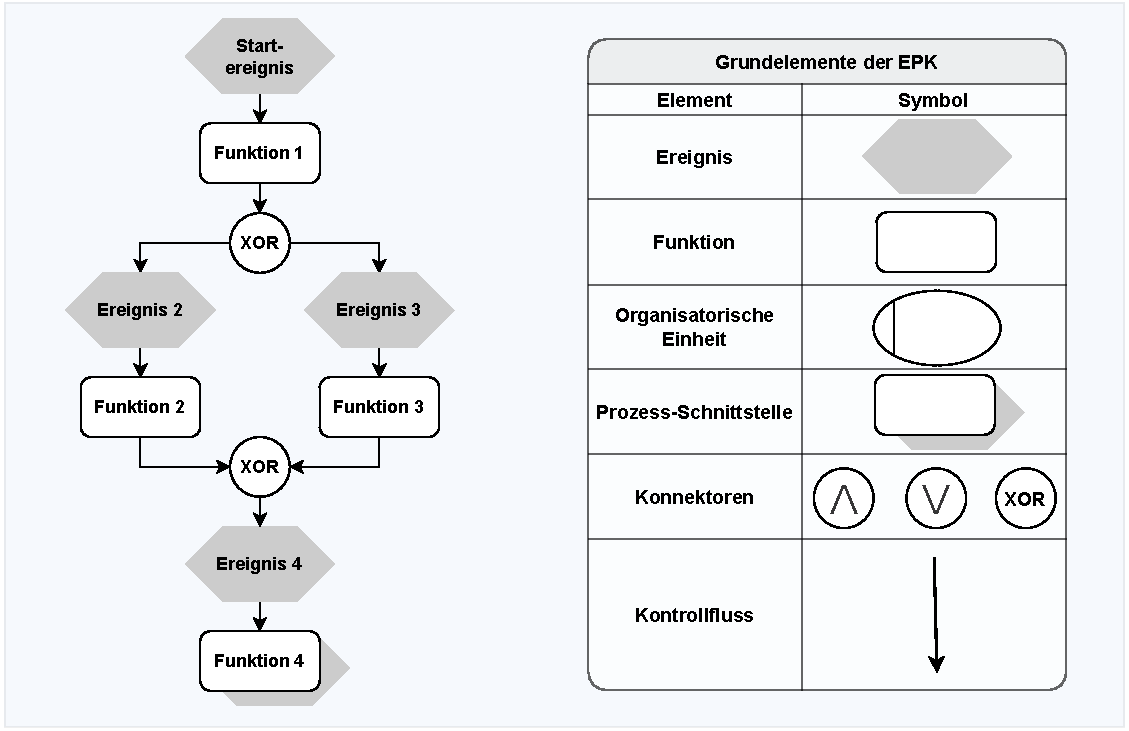
\includegraphics[scale=0.9]{Bilder/Kapitel-5/grundelemente_EPK.pdf}
		\caption{EPK}
		\label{fig:grundelemente_EPK}
	\end{addmargin*}
	\end{addmargin*}
\end{figure}

Abbildung~\ref{fig:grundelemente_EPK} zeigt eine ereignisgesteuerte Prozesskette (EPK) 
\marginline{Beispiel: EPK}
und ihre typischen Elemente und Symbole. EPKs wurden in den 1990er Jahren zur Modellierung von Geschäftsprozessen von Organisationen entwickelt \cite{kel92}. In EPKs gibt es, wie in vielen Prozessmodellierungssprachen, Aktivitäten (hier Funktionen genannt) und lokale Zustände (hier Ereignisse genannt) sowie die Konnektoren UND, ODER und exklusives ODER (XOR), die mögliche Abläufe und ihre Verzweigungen definieren. Es existieren in EPKs weitere Elemente wie Rollen oder notwendige Ressourcen.

Im Kontext der Prozessmodellierung wird das Wort „Ereignis“ leider auf unterschiedliche Weise verwendet. Was hier als „Ereignis“ bezeichnet wird, heißt in anderen Modellierungssprachen als „Bedingung“ oder „lokaler Zustand“.

Etwas moderner als die EPKs sind 
\marginline{Beispiel: BPMN}
Business Process Model and Notation (BPMN)-Diagramme. Diese Modellierungssprache entstand Anfang der 2000er Jahre bei IBM und wird seit 2005 von der Object Management Group (OMG) verwaltet, die auch für die Unified Modeling Language (UML) verantwortlich ist \cite{wes24}. Abbildung~\ref{fig:grundelemente_BPMN} zeigt ein BPMN-Diagramm mit seinen typischen Elementen und Symbolen.

\begin{figure}[!htbp]
	\begin{addmargin*}[0cm]{-\marginparwidth}
	\begin{addmargin*}[0cm]{-\marginparsep}
		\centering
		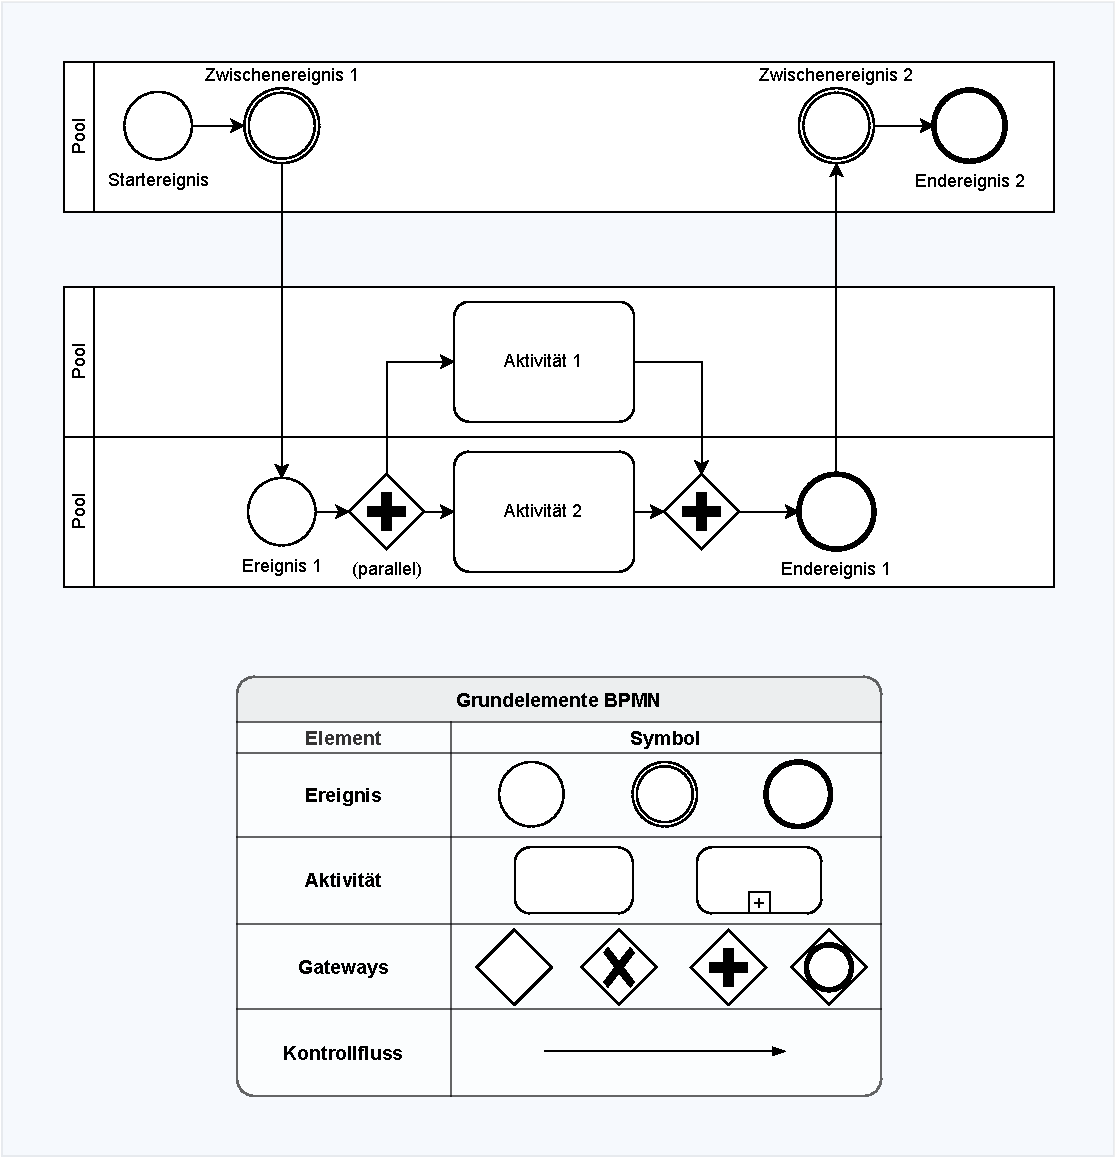
\includegraphics[scale=0.9]{Bilder/Kapitel-5/grundelemente_BPMN.pdf}
		\caption{BPMN}
		\label{fig:grundelemente_BPMN}
	\end{addmargin*}
	\end{addmargin*}
\end{figure}

BPMN bietet eine sehr große Palette an Symbolen, um Geschäftsprozesse detailliert abzubilden. Die zentralen Elemente sind allerdings auch hier Aktivitäten, lokale Zustände (wieder „Ereignisse“ genannt) sowie die Beschreibung des Kontrollflusses durch Pfeile und verschiedene Konnektoren.

\clearpage

\subsection*{Unterscheidung von System, Prozess und Ablauf}

Die Konzepte System, Prozess, Ablauf und weitere werden in der Literatur häufig verwendet, aber oft nicht hinreichend unterschieden. Bei einer formalen Modellierung mit Petrinetzen haben wir die Möglichkeit, diese Begriffe zu präzisieren.

Wenn wir von Realwelt-Modellierung sprechen, dann meinen wir nie die ganze Welt, sondern stets einen Ausschnitt. Wir müssen also festlegen, \textbf{was} wir modellieren wollen, und dabei auch, was nicht, und an welchen Stellen es relevante Schnittstellen gibt zwischen dem behandelten Ausschnitt und dem Rest. Dieser Schritt ist bereits eine erste Abstraktion: Wir abstrahieren von allem, was wir nicht betrachten wollen und reduzieren das gesamte relevante Verhalten dieser Restwelt zu Schnittstellen.


\begin{figure}[!htbp]
	\centering
	\resizebox{\textwidth}{!}{
		\begin{tikzpicture}
			\sffamily % kompletter Text ohne Serifen
			\bfseries % ... fett
			\Huge % ... und größer
			
			% Realwelt/Modell: Rechtecke mit abgerundeten Ecken und transparenter Füllung
			\fill[white!20!black, rounded corners=40pt, opacity=0.1] (-5,0) rectangle (15,20);
			\draw[white!20!black, thick, rounded corners=40pt] (-5,0) rectangle (15,20);
			\node[white!20!black, anchor=south east] at (1,18) {(Real-)Welt};
			
			\fill[FernUni-MI-green, rounded corners=40pt, opacity=0.2] (18,0) rectangle (38,20);
			\draw[FernUni-MI-green, thick, rounded corners=40pt] (18,0) rectangle (38,20);
			\node[FernUni-MI-green, anchor=south east] at (37,18) {Modell};
			
			% System/Systemmodell: Kreise
			%\fill[white, rounded corners=10pt] (5,13) circle (4.5);
			\fill[blue!30!black, rounded corners=10pt, opacity=0.2] (5,13) circle (4.5);
			\draw[blue!30!black, line width=0.5mm] (5,13) circle (4.5);
			\node[blue!30!black] at (5,15) {System};
			
			%\fill[white, rounded corners=10pt] (28,13) circle (4.5);
			\fill[blue!30!black, rounded corners=10pt, opacity=0.2] (28,13) circle (4.5);
			\draw[blue!30!black, line width=0.5mm] (28,13) circle (4.5);
			\node[blue!30!black] at (28,15) {Systemmodell};
			
			% Prozess/Prozessmodell: Rechtecke abgerundet
			\fill[white, rounded corners=15pt] (1.5,10.9) rectangle (8.5,12.1);
			\draw[rounded corners=15pt, line width=0.5mm] (1.5,10.9) rectangle (8.5,12.1);
			\node[] at (5,11.5) {Prozess};
			
			\fill[white, rounded corners=15pt] (24.5,10.9) rectangle (31.5,12.1);
			\draw[rounded corners=15pt, line width=0.5mm] (24.5,10.9) rectangle (31.5,12.1);
			\node[] at (28,11.5) {Prozessmodell};
			
			% Abläufe: Rechtecke abgerundet
			\fill[white] (7,6) rectangle (13.5,8);
			\draw[blue!30!black, line width=0.5mm] (7,6) rectangle (13.5,8);
			\node[blue!30!black] at (10.25,7) {Systemablauf};
			
			\fill[white] (19.5,6) rectangle (29.4,8);
			\draw[blue!30!black, line width=0.5mm] (19.5,6) rectangle (29.4,8);
			\node[blue!30!black] at (24.5,7) {Systemmodellablauf};
			
			\fill[white] (1.9,3) rectangle (8.3,5);
			\draw[line width=0.5mm] (1.9,3) rectangle (8.3,5);
			\node[] at (5,4) {Prozessablauf};
			
			\fill[white] (22.2,3) rectangle (32,5);
			\draw[line width=0.5mm] (22.2,3) rectangle (32,5);
			\node[] at (27.3,4) {Prozessmodellablauf};
			
			% Pfeile
			\draw[red,thick, ->, line width=2mm, -latex] (23.4,13) to (9.5,13);
			\draw[red,thick, ->, line width=2mm, -latex] (24.4,11.5) to (8.6,11.5); 
			\draw[red,thick, ->, line width=2mm, -latex] (19.4,7) to (13.5,7);
			\draw[red,thick, ->, line width=2mm, -latex] (22.1,4) to (8.3,4);
			
			% gestrichelte Linien
			\draw[dashed,blue!30!black, thick, -, line width=1.5mm] (24.7,9.9) to (23,8);
			\draw[dashed,blue!30!black, thick, -, line width=1.5mm] (8.3,9.9) to (10,8);
			\draw[dashed,black, thick, -, line width=1.5mm] (5,10.9) to (5,5);
			\draw[dashed,black, thick, -, line width=1.5mm] (30,10.9) to (30,5);
	\end{tikzpicture}}
	\caption{Modellierung von Systemen, Prozessen und Abläufen}
	\label{fig:v3-system_prozess}
\end{figure}


%Abbildung~\ref{fig:v3-system_prozess} zeigt...\\

Im ausgewählten Weltausschnitt, dem \textbf{System}, 
\marginline{System und Systemmodell}
gibt es vielfältige Aspekte, die mit Verhalten, also möglichen Veränderungen und dafür verantwortlichen Aktivitäten zu tun haben. Auf diese Aspekte konzentrieren wir uns bei der Verhaltensmodellierung, von anderen Aspekten abstrahieren wir. Auf Modellebene gilt es nun, das System zu modellieren mittels eines \textbf{Systemmodells}, in dem mit Elementen einer \textbf{Modellierungssprache} das relevante Systemverhalten nachgebildet wird.

Dieses Verhalten wird -- grob gesagt -- konstituiert durch die \textbf{Abläufe} des Systems. 
\marginline{Systemablauf, Aktivitäten und Aktionen}
Jeder \textbf{Systemablauf} stellt ein tatsächlich mögliches oder ein stattgefundenes Verhalten dar, definiert durch die \textbf{Aktivitäten}, die stattfinden. Wir nennen das Stattfinden einer Aktivität \textbf{Aktion}. Mehrere Aktionen eines Systemablaufs können sich auf dieselbe Aktivität beziehen, wenn diese mehrfach stattfindet. Zwischen den Aktionen eines Systemablaufs gibt es eine Abhängigkeitsbeziehung: Eine Aktion kann erst dann geschehen, wenn zuvor eine andere geschehen ist.

Das Systemmodell bildet das System dann korrekt ab, 
\marginline{Semantik bestimmt das Modellverhalten}
wenn man auch vom Modell Abläufe ableiten kann, die den Systemabläufen entsprechen, also als Modelle der Systemabläufe verstanden werden können. Während der Zusammenhang zwischen System und Systemablauf durch die Realität gegeben ist (im System können diese Abläufe geschehen), wird die Beziehung zwischen Systemmodell und seinen Abläufen durch die Semantik der Modellierungssprache definiert: Sie muss spezifizieren, was wir als Ablauf eines Systemmodells betrachten. Das Modellverhalten ist also nicht mit dem Modell selbst gegeben, sondern wird durch die Semantik passend konstruiert.

\vspace{1mm} %%% für Druck

\phantomsection
\label{text:prozesse_als_teilsysteme}
Auch wenn der Begriff System sehr umfassend ist, 
\marginline{Prozesse als Teilsysteme}
wollen wir nun zwei, im Bereich des Softwareengineering typische Klassen von Systemen genauer anschauen: Die erste, die wir im Folgenden einfach \textbf{Systeme} nennen werden, wird vielleicht durch die Beispiele Aufzugsteuerungssystem, Betriebssystem oder Datenbanksystem ganz gut charakterisiert. Im Softwareengineering aber schaut man insbesondere auch auf \textbf{Prozesse}, die von Systemen unterstützt oder generiert werden können. Formal betrachten wir einen Prozess auch als ein Teilsystem (und damit auch als System) eines größeren Systems. Daher gibt es auch Prozessmodelle, Prozessabläufe und Prozessmodellabläufe, und die Prozessabläufe sollen den Prozessmodellabläufen entsprechen.

\vspace{1mm} %%% für Druck

Typisch für Systeme ist, 
\marginline{(erwünschte) Eigenschaften von Systemen}
dass sie grundsätzlich immer weiter laufen können und nicht irgendwann aufgrund von gegenseitigem Warten verteilter Komponenten, Ressourcenmangel oder Ähnlichem steckenbleiben, also Zustände erreichen, in denen keine weiteren Aktivitäten mehr möglich sind (Deadlocks). Mehr noch, man wird von derartigen Systemen zusätzlich erwarten, dass es stets möglich ist, alle definierten Aktivitäten wieder auszuführen (ein Aufzugsteuerungssystem ist Deadlock-frei, auch wenn eine Etage irgendwann nie wieder erreicht werden kann, aber sicherlich nicht korrekt). Ein System mit dieser Eigenschaft heißt \textbf{lebendig}. Eine vermeint\-liche Möglichkeit, ein System lebendig zu halten, mag man darin sehen, beliebig viele neue Dokumente, Ressourcen, Aufträge, Nachrichten etc. zu generieren, sodass alle Systemkomponenten stets zu tun haben und nicht steckenbleiben. Derartige Systeme haben aber konsequenterweise eine unbeschränkte Menge erreichbarer Zustände, was sie erstens sehr unübersichtlich und unhandlich macht und zweitens ignoriert, dass in der Realität alle Speicher (in einem sehr allgemeinen Sinn) nur eine endliche Kapazität haben. Davon zu abstrahieren, führt schließlich auch zu Fehlern, wie man sie bei der Software-Erstellung kennt. Wir nennen derartige Systeme \textbf{unbeschränkt} und wünschen uns \textbf{beschränkte} Systeme. Deadlock-Freiheit, Lebendigkeit und Beschränktheit findet man als formale Qualitätskriterien wieder auf der Ebene von Systemmodellen.

\vspace{1mm} %%% für Druck

Die typischen Qualitätskriterien von Prozessen 
\marginline{(erwünschte) Eigenschaften von Prozessen}
unterscheiden sich deutlich von denen der Systeme. Zur Motivation dient das Beispiel des Aufzugsteuerungssystems. Wozu dient es? Es soll erlauben, dass jederzeit eine Person in irgendeiner Etage den Knopf drücken kann, irgendwann der Aufzug kommt, die Person einsteigt, in der Aufzugskabine ihr Ziel angibt ... und sie schließlich die gewünschte Etage erreicht. Andere typische Prozesse sind zum Beispiel bei dem System eines Versicherungsunternehmens die Abwicklung eines Schadens von der Schadensmeldung bis zur Auszahlung oder vom Versicherungsantrag bis zum fertigen Vertrag. Typischerweise ist mit einem Prozess ein Ziel verbunden, das irgendeinen Wert (für wen auch immer) hat. Wir erwarten, dass jeder Ablauf des Prozesses -- der durch ein Ereignis wie „Knopfdruck“, „Schadensmeldung“ oder „Versicherungsauftrag“ initiiert wird -- sein Ziel erreicht, wenigstens aber schließlich zu einem gewollten Ende kommt. Ein Prozess soll nicht lebendig oder Deadlock-frei sein, aber steckenbleiben oder unbeschränkte Ressourcen generieren soll er auch nicht. Wir werden später sehen, dass der Begriff „soundness“ auf Modellebene das gewünschte Verhalten von Prozessen ganz gut beschreibt.

\minisec{Definitionen der Begriffe}

\sttpDefinitionskasten{\sttpDefinitionskastenSkalierungsfaktorKapPN}{Definition 5.1: System}{}
{Ein System ist ein physisches oder logisches, existierendes oder gedachtes Regelwerk zu Ausführungen von Aktivitäten des Systems in einzelnen Abläufen.}

\vspace{-\baselineskip} % bei zwei aufeinanderfolgenden Definitionskästen Abstand verkleinern
\vspace{-2mm} % für Druck

\sttpDefinitionskasten{\sttpDefinitionskastenSkalierungsfaktorKapPN}{Definition 5.2: Systemablauf}{}
{Ein Systemablauf besteht aus Aktionen, die Instanzen (Stattfinden von) Aktivitäten sind, samt der kausalen Abhängigkeiten zwischen den Aktionen.}

\vspace{-\baselineskip} % bei zwei aufeinanderfolgenden Definitionskästen Abstand verkleinern
\vspace{-2mm} % für Druck

\sttpDefinitionskasten{\sttpDefinitionskastenSkalierungsfaktorKapPN}{Definition 5.3: Prozess}{}
{Ein Prozess ist ein Systemausschnitt, der eine Menge von Abläufen produzieren kann, welche von einem Startzustand zu einem Endzustand führen (sollen).}

\vspace{-\baselineskip} % bei zwei aufeinanderfolgenden Definitionskästen Abstand verkleinern
\vspace{-2mm} % für Druck

\sttpDefinitionskasten{\sttpDefinitionskastenSkalierungsfaktorKapPN}{Definition 5.4: Prozessablauf}{}
{Ein Prozessablauf ist die einmalige Durchführung eines Prozesses.}

\vspace{-\baselineskip} % für Druck

\subsection*{Verwendung der Modellierungssprachen im Softwareengineering}

Die bereits erwähnten Modellierungssprachen EPK und BPMN sowie UML-Akti\-vi\-täts\-dia\-gramme dienen der Modellierung von Prozessen und finden im Software\-engineering weite Verbreitung, insbesondere bei der Realwelt-Modellierung. Entsprechende Petrinetze sind Workflow-Petrinetze, die wir in den späteren Vorlesungen kennenlernen werden. An ganz anderer Stelle tauchen Verhaltensmodelle im Softwareengineering aber auch auf: Das Verhalten von Objekten, also ihre Zustands\-veränderungen und die Auslöser dafür, werden in Zustandsdiagrammen beschrieben (die diesen zugrundeliegenden State Charts (\cite{har87}) dienen allerdings auch der Realwelt-Modellierung). Wir können diese aber auch als spezielle (sequentielle) Petrinetze interpretieren. Schließlich hat sich für die Modellierung von Objekt\-interaktionen das UML-Sequenzdiagramm bewährt (auch diese Sprache hat ihren Ursprung in einem anderen Bereich, nämlich der Telekommunikation). Jedes derartige Diagramm hat viele Gemeinsamkeiten mit einem Petrinetz-Ablauf, also der Systemmodellablauf-Ebene. 

\clearpage
\section{Vorlesung 2: Modellierung von Verhalten mit Halbordnungen}

Das Verhalten eines Systems besteht - ganz grob ausgedrückt - aus seinen Abläufen. Und ein Ablauf beschreibt, was tatsächlich geschieht oder geschehen ist. Es geht bei der Verhaltensbeschreibung im Allgemeinen natürlich weiter; sie beschreibt auch, was wann geschehen könnte, welche Alternativen möglich sind, wovon sie abhängen usw.

Als Mensch ist man versucht, einen Ablauf immer durch globale Zustände, also Momentaufnahmen, und schrittweise Zustandsänderungen zu beschreiben, also das Verhalten an einem gedachten Zeitstrahl auszurichten. Dies hängt damit zusammen, dass wir als Mensch Verhalten stets nur sequentiell beobachten können, also alles nur nacheinander sehen können, und deshalb Begriffe wie „Zustand“ und „nacheinander“ als grundlegend ansehen. Auch viele Modellierungssprachen folgen diesem Paradigma, sind aber bei großen, komplexen, oft verteilten Systemen nicht wirklich geeignet, um Verhalten tatsächlich verständlich zu machen.

Eine der grundlegenden Ideen der Petrinetz-Theorie ist, 
\marginline{Abhängigkeit zwischen Aktionen statt zeitlichem Nacheinander}
von dieser sequentiellen Sicht abzurücken. Man könnte sagen, ein Petrinetz abstrahiert von Zeit und damit von einem „Nacheinander“ von Aktionen und beschränkt sich auf Abhängigkeiten zwischen Aktionen der Art: Eine Aktion kann nur geschehen, nachdem eine andere geschehen ist, die eine Vorbedingung erst gültig gemacht hat. Richtiger ist allerdings die Argumentation, dass man Zeit gar nicht abstrahieren muss, denn sie existiert auch im System nicht als reale, überall verfügbare Größe. Bestenfalls gibt es Uhren, und wenn man diese zur Verhaltensbeschreibung benötigt, integriert man sie im Modell.

\subsection*{Modellierung eines Ablaufs}

Im Zoo werden Tiere gefüttert, 
\marginline{Beispiel Tierfütterung}
was in der Videovorlesung durch eine Animation dargestellt wird. Diesen konkreten Ablauf können wir folgendermaßen beschreiben:

\begin{addmargin}[25pt]{25pt}
	Die Tierfütterung beginnt damit, dass sich drei Tierpfleger aufmachen die Tiere zu füttern. Sie füttern Löwen, Pinguine, Robben und Affen. Löwen fressen Fleisch. Pinguine und Robben fressen Fisch. Affen fressen Obst. Tierpfleger müssen das jeweilige Futter laden, bevor sie die Tiere füttern. Die gefräßigen Löwen fressen mehr als eine Futterladung. Für ihre Fütterung muss also nachgeladen werden. Die Fütterung endet, wenn alle Tiere versorgt sind.
\end{addmargin}

In Abbildung~\ref{fig:v3-Pinguine_und_Löwen} modellieren wir zunächst den Ablauf durch Aktionen und ihre kausalen Abhängigkeiten.

\clearpage %%% für Druck - absichtlich hier, damit die Einrückung im vorherigen Absatz deutlch ist.

\begin{figure}[!htbp]
	\centering
	\resizebox{1.0\textwidth}{!}{
		\petrinetz{
			
			\sffamily % kompletter Text ohne Serifen
			\Large % kompletter Text größer
			
			\draw[colDummyLine, very thick] (-1,-5) rectangle (25,5);
			
			\node[transition, draw=COLTRANS, minimum height=\PNTransHeight, minimum width=\PNTransWidth, align=center] (t1) at (2,0) {Anfang};
			\node[transition, draw=COLTRANS, minimum height=\PNTransHeight, minimum width=\PNTransWidth, align=center] (t2) at (6,4) {Futter\\laden};
			\node[transition, draw=COLTRANS, minimum height=\PNTransHeight, minimum width=\PNTransWidth, align=center] (t3) at (7,0) {Futter\\laden};
			\node[transition, draw=COLTRANS, minimum height=\PNTransHeight, minimum width=\PNTransWidth, align=center] (t4) at (8,-4) {Futter\\laden};
			\node[transition, draw=COLTRANS, minimum height=\PNTransHeight, minimum width=\PNTransWidth, align=center] (t5) at (10,4) {Löwen\\füttern};
			\node[transition, draw=COLTRANS, minimum height=\PNTransHeight, minimum width=\PNTransWidth, align=center] (t6) at (12,0) {Pinguine\\füttern};
			\node[transition, draw=COLTRANS, minimum height=\PNTransHeight, minimum width=\PNTransWidth, align=center] (t7) at (16,-4) {Affen\\füttern};
			\node[transition, draw=COLTRANS, minimum height=\PNTransHeight, minimum width=\PNTransWidth, align=center] (t8) at (14,4) {Futter\\laden};
			\node[transition, draw=COLTRANS, minimum height=\PNTransHeight, minimum width=\PNTransWidth, align=center] (t9) at (17,0) {Robben\\füttern};
			\node[transition, draw=COLTRANS, minimum height=\PNTransHeight, minimum width=\PNTransWidth, align=center] (t10) at (18,4) {Löwen\\füttern};
			\node[transition, draw=COLTRANS, minimum height=\PNTransHeight, minimum width=\PNTransWidth, align=center] (t11) at (22,0) {Ende};
			
			% Kanten (Pfeile)
			\draw[post] (t1) -- (t2);
			\draw[post] (t1) -- (t3);    
			\draw[post] (t1) -- (t4);
			\draw[post] (t2) -- (t5);
			\draw[post] (t5) -- (t8);
			\draw[post] (t8) -- (t10);
			\draw[post] (t10) -- (t11);
			\draw[post] (t3) -- (t6);
			\draw[post] (t6) -- (t9);
			\draw[post] (t9) -- (t11);
			\draw[post] (t4) -- (t7);
			\draw[post] (t7) -- (t11);
		}
	}
	\caption{Erster Schritt der Modellierung des Ablaufs der Tierfütterung}
	\label{fig:v3-Pinguine_und_Löwen}
\end{figure}


\minisec{Aktionen}
Jeder Knoten im Diagramm stellt eine Aktion dar, die im Ablauf durchgeführt
wird. Sie haben in diesem Diagramm die folgenden Namen:
\begin{itemize}
	\item \textbf{Anfang} (meist beginnt jeder Ablauf eines Prozesses mit einem „Anfang“)
	
	\item \textbf{Futter laden} (für Löwen, Pinguine, Robben und Affen)
	
	\item \textbf{Löwen füttern} (zweimal, da ein Nachladen erforderlich ist)
	
	\item \textbf{Pinguine füttern}
	
	\item \textbf{Robben füttern}
	
	\item \textbf{Affen füttern}
	
	\item \textbf{Ende} (alle Tiere wurden gefüttert und der Ablauf ist beendet)
\end{itemize}

Da mehrere Aktionen denselben Namen tragen, können wir sie nicht einfach mit ihren Namen identifizieren, die Aktion „Löwen füttern“ existiert z.B. nicht eindeutig.

\minisec{Kausale Ordnung}
Gerichtete Kanten 
\marginline{Kanten und Kausalität}
geben im Ablaufdiagramm die direkte \textbf{Kausalität}\footnote{Der Begriff „Kausalität“ ist nicht immer korrekt, denn die Tiere werden nicht gefüttert, \textbf{weil} Futter geladen wurde, eher anders herum.} zwischen den Aktionen wieder: Eine Kante von einer Aktion zu einer anderen bedeutet, dass die erste Aktion abgeschlossen sein muss, bevor die nachfolgende Aktion beginnen kann. Zum Beispiel muss die Aktion „Futter laden“ für die Affen abgeschlossen sein, bevor das „Affen füttern“ beginnen kann. Aktionen, deren kausale Ordnung nicht festgelegt ist, sind \textbf{unabhängig} voneinander. Es ist keine Reihenfolge festgelegt! 

\pagebreak

Im Diagramm gibt es (entsprechend der Ablaufbeschreibung) folgende kausale Zusammenhänge:
\begin{itemize}
	\item „Anfang“ $\rightarrow$ „Futter laden“ $\rightarrow$ „Löwen füttern“ $\rightarrow$ „Futter laden“ $\rightarrow$ „Löwen füttern“ $\rightarrow$ „Ende“
	
	\item „Anfang“ $\rightarrow$ „Futter laden“ $\rightarrow$ „Pinguine füttern“ $\rightarrow$ „Robben füttern“ $\rightarrow$ „Ende“
	
	\item „Anfang“ $\rightarrow$ „Futter laden“ $\rightarrow$ „Affen füttern“ $\rightarrow$ „Ende“
\end{itemize}

Neben den direkten kausalen Abhängigkeiten betrachten wir später eine kausale Halbordnung, die weitere Abhängigkeiten umfasst. 

%\subsubsection*{Modellierung eines Ablaufs (2): Bedingungen, Marken}

\minisec{Bedingungen}

Im einem weiteren Schritt wird das Ablaufdiagramm aus Abbildung~\ref{fig:v3-Pinguine_und_Löwen} überführt in ein erstes Petrinetz. Das erreichen wir durch folgende Änderungen und Ergänzungen: Wenn eine Aktion erst nach einer anderen Aktion geschehen kann, sie also kausal von der anderen Aktion abhängt, dann gibt es dafür stets einen Grund: Eine Voraussetzung der zweiten Aktion wird durch die erste Aktion geschaffen. In anderen Worten: Durch die erste Aktion wird eine Bedingung erfüllt, die zugleich Bedingung für die zweite Aktion ist.

Derartige Bedingungen fügen wir im Diagramm ein 
\marginline{ein erstes Petrinetz}
und machen so die Gründe für die kausalen Abhängigkeiten explizit (Abbildung~\ref{fig:v3-Ablaufdiagramm_1}). Graphisch werden Bedingungen durch Kreise dargestellt. Die Kanten verbinden nunmehr nicht Aktionen, sondern Aktionen und Bedingungen. Jede Bedingung entspricht
\begin{itemize}
	\item einer Kante im Ursprungsdiagramm (dann hat sie genau eine eingehende und genau eine ausgehende Kante) oder
	\item der Anfangsbedingung, die beschreibt, was anfangs gilt und für die Anfangs\-aktion Voraussetzung ist (dann hat sie keine eingehende und genau eine ausgehende Kante) oder
	\item der Endbedingung, die nach der letzten Aktion erfüllt ist (dann hat sie genau eine eingehende und keine ausgehende Kante).
\end{itemize}

Wir haben aus Platzgründen nur bei einigen Bedingungen textuell beschrieben, wofür sie, bezogen auf das modellierte System, stehen.


\begin{figure}[!htbp]
	\centering
	\resizebox{1.0\textwidth}{!}{
		\petrinetz{
			\sffamily % kompletter Text ohne Serifen
			\Large % kompletter Text größer
			
			\draw[colDummyLine, very thick] (-1,-5) rectangle (25,5);
			
			% Places (Stellen in Grün)
			{
				\color{COLPLACE}
				
				\node[place, tokens=1, minimum size=\PNPlaceSize, label=above:{\rotatebox{90}{Anfangsbedingung}}] (A) at (0,0) {};
				\node[place, minimum size=\PNPlaceSize, label=above:{\rotatebox{90}{Bereit zum Futter laden}}] (B) at (4,2) {};
				\node[place, minimum size=\PNPlaceSize] (C) at (4.5,0) {};
				\node[place, minimum size=\PNPlaceSize] (D) at (4.5,-2) {};
				\node[place, minimum size=\PNPlaceSize, label=above:{\rotatebox{90}{Löwenfutter geladen}}] (E) at (8,4) {}; 
				\node[place, minimum size=\PNPlaceSize, label=above:{\rotatebox{90}{Löwenfutter geladen}}] (E2) at (16,4) {}; 
				\node[place, minimum size=\PNPlaceSize] (F) at (9.5,0) {}; 
				\node[place, minimum size=\PNPlaceSize] (G) at (12,-4) {}; 
				\node[place, minimum size=\PNPlaceSize, label=above:{\rotatebox{90}{Bereit zum Futter laden}}] (H) at (12,4) {}; 
				\node[place, minimum size=\PNPlaceSize] (I) at (14.5,0) {}; 
				\node[place, minimum size=\PNPlaceSize] (L) at (19.5,0) {}; 
				\node[place, minimum size=\PNPlaceSize, label=above:{\rotatebox{90}{Endbedingung}}] (Z) at (24,0) {}; 
				\node[place, minimum size=\PNPlaceSize, label=above:{\rotatebox{90}{Bereit zum Futter laden}}] (H2) at (20,2) {}; 
				\node[place, minimum size=\PNPlaceSize] (J2) at (19,-2) {};
			}
			
			% Transitions (Transitionen in Blau)
			\node[transition, draw=COLTRANS, minimum height=\PNTransHeight, minimum width=\PNTransWidth, align=center] (t1) at (2,0) {Anfang}; 
			\node[transition, draw=COLTRANS, minimum height=\PNTransHeight, minimum width=\PNTransWidth, align=center] (t2) at (6,4) {\textcolor{COLRED}{\textbf{Fleisch}}\\laden}; 
			\node[transition, draw=COLTRANS, minimum height=\PNTransHeight, minimum width=\PNTransWidth, align=center] (t3) at (7,0) {\textcolor{COLRED}{\textbf{Fisch}}\\laden}; 
			\node[transition, draw=COLTRANS, minimum height=\PNTransHeight, minimum width=\PNTransWidth, align=center] (t4) at (8,-4) {\textcolor{COLRED}{\textbf{Obst}}\\laden}; 
			\node[transition, draw=COLTRANS, minimum height=\PNTransHeight, minimum width=\PNTransWidth, align=center] (t5) at (10,4) {Löwen\\füttern}; 
			\node[transition, draw=COLTRANS, minimum height=\PNTransHeight, minimum width=\PNTransWidth, align=center] (t6) at (12,0) {Pinguine\\füttern}; 
			\node[transition, draw=COLTRANS, minimum height=\PNTransHeight, minimum width=\PNTransWidth, align=center] (t7) at (16,-4) {Affen\\füttern}; 
			\node[transition, draw=COLTRANS, minimum height=\PNTransHeight, minimum width=\PNTransWidth, align=center] (t8) at (14,4) {\textcolor{red!80!black}{\textbf{Fleisch}}\\laden}; 
			\node[transition, draw=COLTRANS, minimum height=\PNTransHeight, minimum width=\PNTransWidth, align=center] (t9) at (17,0) {Robben\\füttern}; 
			\node[transition, draw=COLTRANS, minimum height=\PNTransHeight, minimum width=\PNTransWidth, align=center] (t10) at (18,4) {Löwen\\füttern}; 
			\node[transition, draw=COLTRANS, minimum height=\PNTransHeight, minimum width=\PNTransWidth, align=center] (t11) at (22,0) {Ende};
			
			% Kanten (Pfeile)
			\draw[post] (A) -- (t1); 
			\draw[post] (t1) -- (B); 
			\draw[post] (t1) -- (C); 
			\draw[post] (t1) -- (D); 
			\draw[post] (B) -- (t2); 
			\draw[post] (C) -- (t3); 
			\draw[post] (D) -- (t4); 
			\draw[post] (t2) -- (E); 
			\draw[post] (t3) -- (F); 
			\draw[post] (t4) -- (G); 
			\draw[post] (G) -- (t7); 
			\draw[post] (E) -- (t5); 
			\draw[post] (t5) -- (H); 
			\draw[post] (H) -- (t8); 
			\draw[post] (t8) -- (E2); 
			\draw[post] (E2) -- (t10); 
			\draw[post] (t10) -- (H2); 
			\draw[post] (H2) -- (t11); 
			\draw[post] (t11) -- (Z); 
			\draw[post] (t9) -- (L); 
			\draw[post] (t7) -- (J2); 
			\draw[post] (J2) -- (t11); 
			\draw[post] (L) -- (t11); 
			\draw[post] (F) -- (t6); 
			\draw[post] (t6) -- (I); 
			\draw[post] (I) -- (t9); 
		}
	}
	\caption{Zweiter Schritt der Modellierung des Ablaufs der Tierfütterung}
	\label{fig:v3-Ablaufdiagramm_1}
\end{figure}

\minisec{Aktionen und Aktivitäten}

Aktionen beschreiben das Stattfinden von Aktivitäten, doch letztere kennen wir an dieser Stelle noch nicht. Naheliegend wäre die Beschriftungen der Aktionen als Aktivitäten zu verwenden. Aber betreffen zwei Aktionen mit demselben Namen stets dieselbe Aktivität? Um dies zu beantworten, helfen die Bedingungen.

In dem Diagramm aus Abbildung~\ref{fig:v3-Pinguine_und_Löwen} sind vier Aktionen beschriftet mit „Futter laden“. Tatsächlich unterscheiden wir aber, für welche Tiergattung das Futter geladen wurde. 

\pagebreak

In Abbildung~\ref{fig:v3-Ablaufdiagramm_1} gibt es zwei nachfolgende Bedingungen „Löwenfutter geladen“, 
\marginline{Aktivitäten können mehrfach vorkommen}
für die weiteren beiden Bedingungen wären „Affenfutter geladen“ und „Pinguinfutter geladen“ passende Namen. Die beiden Aktionen „Löwen füttern“ haben dieselben Bedingungen vor und nach der Aktion und entsprechen daher derselben Aktivität. Entsprechend wurden einige Aktionen im neuen Diagramm umbenannt; die Namen entsprechen jetzt genau den Aktivitäten.

Manch einer mag versucht sein, die beiden Aktionen „Fleisch laden“ und die beiden Aktionen „Löwen füttern“ zusammenzufassen und die Kanten durch einen Zyklus zu ersetzen. Dies ist aber auf Ablaufebene unzulässig, denn jede Aktion beschreibt das \textbf{einmalige} Stattfinden einer Aktivität.


\minisec{Marken}

Wenn sich eine \textbf{Marke} (schwarzer Punkt) in einem Kreis befindet, bedeutet dies, dass diese Bedingung gerade erfüllt ist und die nächste Aktion anschließend ausgeführt wird. Durch die Aktion „Anfang“ verschwindet die Marke von der Anfangs\-bedingung und neue Marken entstehen auf den drei nachfolgenden Bedingungen; nun können die nachfolgenden Aktionen stattfinden.


\minisec{Sequentielle Beobachtungen}

Wenn wir diesen Ablauf, also einen Fütterungsvorgang, in der realen Welt beobachten und dokumentieren, welche Aktionen wir nacheinander sehen, erhalten wir eine \textbf{sequentielle Beobachtung}. Diese lässt sich als \textbf{Ereignisprotokoll} (Event-Log) darstellen, zum Beispiel wie folgt:

\textbf{Anfang, Fleisch laden, Obst laden, Affen füttern, Fisch laden, Pinguine füttern, Robben füttern, Löwen füttern, Fleisch laden, Löwen füttern, Ende}

Man erkennt, 
\marginline{sequentielle Beobachtungen vs. Abläufe}
dass Abhängigkeiten (z.B. „Affen füttern“ nach „Obst laden“) in dieser Sequenz beachtet wurden, aber die Reihenfolge in der Sequenz nicht in allen Fällen Abhängigkeit repräsentiert. Vielfach wird argumentiert, dass eine derartige Sequenz einen Ablauf besser repräsentiert, weil doch zwischen je zwei Aktionen wenigstens die zeitliche Ordnung existiert. Tatsächlich ist diese Sichtweise aber wenig zielführend, insbesondere wenn man Aspekte wie Gleichzeitigkeit einbezieht oder beobachtet, dass Aktionen selbst eine zeitliche Ausdehnung haben, also zu einem späteren Zeitpunkt enden als sie beginnen. Und sie widerspricht der Einsicht, dass quantifizierbare Zeit in der Realität nicht existiert, sondern erst durch Uhren hinzugedichtet wird.

Deshalb, und das ist wichtig, gilt: Eine sogenannte sequentielle Beobachtung eines Ablaufs entspricht nicht dem Ablauf selbst. Ein Ablauf hat meist mehrere denkbare Ereignisprotokolle - und ein Ereignisprotokoll kann auch zu mehreren Abläufen gehören.


\minisec{Petrinetze}

Bisher haben wir die Realwelt beschrieben. Jetzt wollen wir auf die Modellierungssprache eingehen und verwenden deshalb neue Begriffe, die das verdeutlichen.


\begin{figure}[!htbp]
	\centering
	\resizebox{1.0\textwidth}{!}{
		\petrinetz{
			\Large % kompletter Text größer
			
			\draw[colDummyLine, very thick] (-1,-5) rectangle (25,5);
			
			% Places (Stellen in Grün)
			{
				\color{COLPLACE}
				
				\node[place, tokens=1, minimum size=\PNPlaceSize, label=above:{$A$}] (A) at (0,0) {}; 
				\node[place, minimum size=\PNPlaceSize, label=above:{$B$}] (B) at (4,2) {}; 
				\node[place, minimum size=\PNPlaceSize, label=above:{$C$}] (C) at (4.5,0) {}; 
				\node[place, minimum size=\PNPlaceSize, label=above:{$D$}] (D) at (4.5,-2) {}; 
				\node[place, minimum size=\PNPlaceSize, label=above:{$E$}] (E) at (8,4) {}; 
				\node[place, minimum size=\PNPlaceSize, label=above:{$E$}] (E2) at (16,4) {}; 
				\node[place, minimum size=\PNPlaceSize, label=above:{$F$}] (F) at (9.5,0) {}; 
				\node[place, minimum size=\PNPlaceSize, label=above:{$G$}] (G) at (12,-4) {}; 
				\node[place, minimum size=\PNPlaceSize, label=above:{$B$}] (H) at (12,4) {}; 
				\node[place, minimum size=\PNPlaceSize, label=above:{$I$}] (I) at (14.5,0) {}; 
				\node[place, minimum size=\PNPlaceSize, label=above:{$C$}] (L) at (19.5,0) {}; 
				\node[place, minimum size=\PNPlaceSize, label=above:{$Z$}] (Z) at (24,0) {}; 
				\node[place, minimum size=\PNPlaceSize, label=above:{$B$}] (H2) at (20,2) {}; 
				\node[place, minimum size=\PNPlaceSize, label=above:{$D$}] (J2) at (19,-2) {};
			}
			
			% Transitions (Transitionen in Blau)
			\node[transition, label=above:$a$, draw=COLTRANS, minimum height=\PNTransHeight, minimum width=\PNTransWidth, align=center] (t1) at (2,0) {$t_{1}$}; 
			\node[transition, label=above:$b$, draw=COLTRANS, minimum height=\PNTransHeight, minimum width=\PNTransWidth, align=center] (t2) at (6,4) {$t_{2}$}; 
			\node[transition, label=above:$c$, draw=COLTRANS, minimum height=\PNTransHeight, minimum width=\PNTransWidth, align=center] (t3) at (7,0) {$t_{3}$}; 
			\node[transition, label=above:$d$, draw=COLTRANS, minimum height=\PNTransHeight, minimum width=\PNTransWidth, align=center] (t4) at (8,-4) {$t_{4}$}; 
			\node[transition, label=above:$e$, draw=COLTRANS, minimum height=\PNTransHeight, minimum width=\PNTransWidth, align=center] (t5) at (10,4) {$t_{5}$}; 
			\node[transition, label=above:$f$, draw=COLTRANS, minimum height=\PNTransHeight, minimum width=\PNTransWidth, align=center] (t6) at (12,0) {$t_{6}$}; 
			\node[transition, label=above:$g$, draw=COLTRANS, minimum height=\PNTransHeight, minimum width=\PNTransWidth, align=center] (t7) at (16,-4) {$t_{7}$}; 
			\node[transition, label=above:$b$, draw=COLTRANS, minimum height=\PNTransHeight, minimum width=\PNTransWidth, align=center] (t8) at (14,4) {$t_{8}$}; 
			\node[transition, label=above:$h$, draw=COLTRANS, minimum height=\PNTransHeight, minimum width=\PNTransWidth, align=center] (t9) at (17,0) {$t_{9}$}; 
			\node[transition, label=above:$e$, draw=COLTRANS, minimum height=\PNTransHeight, minimum width=\PNTransWidth, align=center] (t10) at (18,4) {$t_{10}$}; 
			\node[transition, label=above:$z$, draw=COLTRANS, minimum height=\PNTransHeight, minimum width=\PNTransWidth, align=center] (t11) at (22,0) {$t_{11}$};
			
			% Kanten (Pfeile)
			\draw[post] (A) -- (t1); 
			\draw[post] (t1) -- (B); 
			\draw[post] (t1) -- (C); 
			\draw[post] (t1) -- (D); 
			\draw[post] (B) -- (t2); 
			\draw[post] (C) -- (t3); 
			\draw[post] (D) -- (t4); 
			\draw[post] (t2) -- (E); 
			\draw[post] (t3) -- (F); 
			\draw[post] (t4) -- (G); 
			\draw[post] (G) -- (t7); 
			\draw[post] (E) -- (t5); 
			\draw[post] (t5) -- (H); 
			\draw[post] (H) -- (t8); 
			\draw[post] (t8) -- (E2); 
			\draw[post] (E2) -- (t10); 
			\draw[post] (t10) -- (H2); 
			\draw[post] (H2) -- (t11); 
			\draw[post] (t11) -- (Z); 
			\draw[post] (t9) -- (L); 
			\draw[post] (t7) -- (J2); 
			\draw[post] (J2) -- (t11); 
			\draw[post] (L) -- (t11); 
			\draw[post] (F) -- (t6); 
			\draw[post] (t6) -- (I); 
			\draw[post] (I) -- (t9); 
		}
	}
	\caption{Formalisiertes Ablaufdiagramm}
	\label{fig:v3-Ablaufdiagramm_formalisierung}
\end{figure}


Die Symbole 
\marginline{Label}
in den Aktionen wurden in Abbildung~\ref{fig:v3-Ablaufdiagramm_formalisierung} durch eindeutige Elemente $t_{1}$ bis $t_{11}$ ersetzt. Die Beschriftungen der Aktionen machen nach wie vor deutlich, welche Aktivität jeweils ausgeführt wird. Man nennt sie „Label“. Die entsprechenden Kästchen nennen wir fortan „Transitionen“.
\marginline{Transitionen}
Wir haben hier also eine Menge von Transitionen $\{t_1 \ldots t_{11}\}$.

Entsprechendes kann man für die Bedingungen machen und ihnen eindeutige Namen geben. 
\marginline{Stellen}
Zwei Bedingungen sind mit „E“ beschriftet, drei mit „B“ usw. Dies des\-wegen, weil sie in der Realwelt jeweils denselben lokalen Zustand repräsentieren. Die eindeutigen Namen (hier nicht vergeben) werden im Modell zu „Stellen“.

\subsection*{Halbordnung}
Bevor wir uns nun genauer mit Stellen und Transitionen beschäftigen, gehen wir einen Schritt weiter und studieren die Abhängigkeitsbeziehungen zwischen Aktionen. Wenn man sich nicht auf die unmittelbare Abhängigkeit (durch Kanten dargestellt) beschränkt, sondern beliebige kausale Zusammenhänge formalisieren will, erhält man eine Halbordnung. Zudem kann man die Bedingungen in die Formalisierung mit einbeziehen.

\sttpDefinitionskasten{\sttpDefinitionskastenSkalierungsfaktorKapPN}{Definition 5.5: (irreflexive) Halbordnung}{Eine (irreflexive) Halbordnung ist eine Relation auf einer Menge, die \textbf{transitiv}, \textbf{irreflexiv} und \textbf{asymmetrisch} ist.}{
	Im Kontext der Prozessmodellierung werden durch eine Halbordnung die (kausalen) Abhängigkeiten zwischen Aktionen eines Ablaufs bzw. zwischen Aktionen und relevanten Bedingungen dargestellt. \\
	
	\textbf{Formal:}
	
	Eine Menge $M$ mit einer Relation $R \subseteq M \times M$ ist eine Halbordnung, wenn gilt:
	
	\begin{itemize}
		\item \textbf{Transitivität:} Für alle $a, b, c \in M$ gilt:
		\[
		(a, b) \in R \ \text{und} \ (b, c) \in R \ \implies \ (a, c) \in R.
		\]
		\item \textbf{Irreflexivität:} Für alle $a \in M$ gilt:
		\[
		(a, a) \notin R.
		\]
		\item \textbf{Asymmetrie:} Für alle $a, b \in M$ gilt:
		\[
		(a, b) \in R \ \implies \ (b, a) \notin R.
		\]
	\end{itemize}
	
	Anmerkung: Asymmetrie folgt aus Transitivität und Irreflexivität, zudem folgt Irreflexivität aus Asymmetrie.
}

Im Diagramm 
\marginline{Kausalitäts\-relation ist eine Halbordnung}
aus Abbildung~\ref{fig:v3-geordnet-und-nicht-geordnet} repräsentiert die Menge $M$ die Transitionen, die für Aktionen stehen. Die Menge $F$ besteht aus allen Paaren $(a,b) \in M \times M$, für die eine gerichtete Kante von $a$ nach $b$ führt. Kausale Abhängigkeiten bestehen aber nicht nur zwischen zwei unmittelbar benachbarten Knoten, sondern auch dann, wenn ein gerichteter Pfad von einem Knoten zu einem anderen Knoten führt. Formal wird diese Abhängigkeit definiert durch die Halbordnung $R \subseteq M \times M$, definiert durch $R = F^{+}$, wobei $F^{+}$ die kleinste transitive Relation ist, die $F$ enthält. Statt $(a,b) \in R$ schreiben wir auch $a\prec_R b$ oder $a\prec b$, wenn der Bezug zu $R$ klar ist. 

\pagebreak %%% für Druck

Es gilt:
\begin{itemize}
	\item $t_1 \prec t_2$, denn es führt eine Kante von $t_1$ nach $t_2$. Deshalb geschieht $t_2$ nach $t_1$.
	\item $t_1 \prec t_{10}$, denn es führt ein gerichteter Pfad von $t_1$ nach $t_{10}$. Deshalb geschieht auch $t_{10}$ nach $t_1$.
	\item Weder $t_4 \prec t_5$ noch $t_5 \prec t_4$, denn es gibt keinen gerichteten Pfad von $t_4$ nach $t_5$ oder von $t_5$ nach $t_4$. Deshalb sind diese Aktionen unabhängig voneinander und geschehen nebenläufig.
\end{itemize}

\vspace{\baselineskip} %%% für Druck
\vspace{1em} %%% für Druck

\begin{figure}[!htbp]
	\centering
	\resizebox{1.0\textwidth}{!}{
		\petrinetz{
			\Large % kompletter Text größer
			
			\draw[colDummyLine, very thick] (-1,-5) rectangle (25,5);
			
			\definecolor{hellblau}{RGB}{204,230,230}
			\definecolor{hellrosa}{RGB}{250,204,209}
			
			\draw[-, hellblau, line width=8pt] (2,0) -- (18,4);
			\fill[hellblau] (2,0) circle (1.6);
			\fill[hellblau] (18,4) circle (1.6);
			
			\draw[-, hellrosa, dashed, line width=8pt] (8,-4) -- (10,4);
			\fill[hellrosa] (10,4) circle (1.6);
			\fill[hellrosa] (8,-4) circle (1.6);
			
			% Transitionen (Transitionen in Blau)
			\node[transition, label=above:$a$, draw=COLTRANS, minimum height=\PNTransHeight, minimum width=\PNTransWidth, align=center] (t1) at (2,0) {$t_1$};
			\node[transition, label=above:$b$, draw=COLTRANS, minimum height=\PNTransHeight, minimum width=\PNTransWidth, align=center] (t2) at (6,4) {$t_2$};
			\node[transition, label=above:$c$, draw=COLTRANS, minimum height=\PNTransHeight, minimum width=\PNTransWidth, align=center] (t3) at (7,0) {$t_3$};
			\node[transition, label=above:$d$, draw=COLTRANS, minimum height=\PNTransHeight, minimum width=\PNTransWidth, align=center] (t4) at (8,-4) {$t_4$};
			\node[transition, label=above:$e$, draw=COLTRANS, minimum height=\PNTransHeight, minimum width=\PNTransWidth, align=center] (t5) at (10,4) {$t_5$};
			\node[transition, label=above:$f$, draw=COLTRANS, minimum height=\PNTransHeight, minimum width=\PNTransWidth, align=center] (t6) at (12,0) {$t_6$};
			\node[transition, label=above:$g$, draw=COLTRANS, minimum height=\PNTransHeight, minimum width=\PNTransWidth, align=center] (t7) at (16,-4) {$t_7$};
			\node[transition, label=above:$b$, draw=COLTRANS, minimum height=\PNTransHeight, minimum width=\PNTransWidth, align=center] (t8) at (14,4) {$t_8$};
			\node[transition, label=above:$h$, draw=COLTRANS, minimum height=\PNTransHeight, minimum width=\PNTransWidth, align=center] (t9) at (17,0) {$t_9$};
			\node[transition, label=above:$e$, draw=COLTRANS, minimum height=\PNTransHeight, minimum width=\PNTransWidth, align=center] (t10) at (18,4) {$t_{10}$};
			\node[transition, label=above:$z$, draw=COLTRANS, minimum height=\PNTransHeight, minimum width=\PNTransWidth, align=center] (t11) at (22,0) {$t_{11}$};
			
			% Kanten (angepasste Pfeile)
			\draw[post] (t1) -- (t2);
			\draw[post] (t1) -- (t3);
			\draw[post] (t1) -- (t4);
			\draw[post] (t2) -- (t5);
			\draw[post] (t3) -- (t6);
			\draw[post] (t4) -- (t7);
			\draw[post] (t5) -- (t8);
			\draw[post] (t8) -- (t10);
			\draw[post] (t6) -- (t9);
			\draw[post] (t7) -- (t11);
			\draw[post] (t9) -- (t11);
			\draw[post] (t10) -- (t11);
		}
	}
	\caption{Geordnete und nicht geordnete (d.h. unabhängige) Elemente}
	\label{fig:v3-geordnet-und-nicht-geordnet}
\end{figure}

\vspace{1em} %%% für Druck

Nun müssen wir noch begründen, dass es sich bei der Relation $R$ tatsächlich um eine Halbordnung handelt.

\begin{itemize}
	\setlength{\itemsep}{2mm} %%% für Druck
	
	\item \textbf{Transitivität}\\
	Wenn ein gerichteter Pfad von einem Knoten $a$ zu einem Knoten $b$ führt und ein weiterer gerichteter Pfad von $b$ zu einem Knoten $c$, dann ist die Kombination dieser Pfade ein gerichteter Pfad von $a$ noch $c$.
	
	\item \textbf{Irreflexivität}\\
	Kein gerichteter Pfad führt von einem Knoten $a$ zum Knoten $a$ zurück, denn sonst wäre das Geschehen von $a$ Voraussetzung dafür, dass $a$ geschieht, und $a$ könnte deshalb nie geschehen. Dies erklärt auch, warum die Aktionen der Löwenfütterung zweimal vorkommen. 
	
	\item \textbf{Asymmetrie}\\
	Wenn ein gerichteter Pfad von einem Knoten $a$ zu einem Knoten $b$ führt, dann kann kein gerichteter Pfad von $b$ zurück zu $a$ führen. Aktionen können also nicht gegenseitig voneinander abhängen. Insbesondere gibt es keine Kreise aus gerichteten Kanten.
\end{itemize}

\pagebreak

\subsection*{Vollordnung}

Wir haben bereits sequentielle Beobachtungen von Abläufen erwähnt. 
\marginline{sequentielle Beobachtung ist eine Vollordnung}
Diese können Beobachtungen eines Menschen sein oder in einem Protokoll automatisch festgehaltene Aktionen (dann heißen sie Ereignisprotokolle, und das Wort "`Ereignis"' steht hier für Aktion). In beiden Fällen erfolgt diese Beobachtung lokal und hat umgekehrt keinen Einfluss auf den Ablauf selbst. Entsprechende Sequenzen entstehen aber auch, wenn der Ablauf nur die logischen Abhängigkeiten widerspiegelt, aber eine nicht modellierte sequentielle Instanz, zum Beispiel eine Person, tatsächlich die Aktionen nacheinander ausführt.

Im Gegensatz zu einer Halbordnung stehen bei einer Vollordnung je zwei verschiedene Elemente in einer Ordnungsbeziehung.

\sttpDefinitionskasten{\sttpDefinitionskastenSkalierungsfaktorKapPN}{Definition 5.6: Vollordnung}{}{Eine Halbordnung, in der für je zwei Elemente $a, b$ gilt: \[a < b \quad \text{oder}\quad a = b \quad \text{oder}\quad a > b\] wird als Vollordnung bezeichnet.}

\subsection*{Linearisierung einer Halbordnung}

Um von einem halbgeordneten Ablauf zu einer kompatiblen Vollordnung zu kommen, müssen wir eine vollständige, sequentielle Reihenfolge aller Aktionen festlegen. Dies geschieht durch eine sogenannte Linearisierung, bei der alle Aktionen in eine Reihenfolge gebracht werden, ohne die kausalen Abhängigkeiten zu verletzen.


\begin{figure}[!htbp]
	\centering
	\resizebox{1.0\textwidth}{!}{
		\petrinetz{
			\Large % kompletter Text größer
			
			\draw[colDummyLine, very thick] (-1,-5) rectangle (25,5);
			
			% Transitions (Transitionen in Blau)
			\node[transition, label=above:$a$, draw=COLTRANS, minimum height=\PNTransHeight, minimum width=\PNTransWidth, align=center] (t1) at (2,0) {$t_1$};
			\node[transition, label=above:$b$, draw=COLTRANS, minimum height=\PNTransHeight, minimum width=\PNTransWidth, align=center] (t2) at (6,4) {$t_2$};
			\node[transition, label={[anchor=south west] $c$}, draw=COLTRANS, minimum height=\PNTransHeight, minimum width=\PNTransWidth, align=center] (t3) at (7,0) {$t_3$};
			\node[transition, label=below:$d$, draw=COLTRANS, minimum height=\PNTransHeight, minimum width=\PNTransWidth, align=center] (t4) at (8,-4) {$t_4$};
			\node[transition, label=above:$e$, draw=COLTRANS, minimum height=\PNTransHeight, minimum width=\PNTransWidth, align=center] (t5) at (10,4) {$t_5$};
			\node[transition, label=above:$f$, draw=COLTRANS, minimum height=\PNTransHeight, minimum width=\PNTransWidth, align=center] (t6) at (12,0) {$t_6$};
			\node[transition, label=below:$g$, draw=COLTRANS, minimum height=\PNTransHeight, minimum width=\PNTransWidth, align=center] (t7) at (16,-4) {$t_7$};
			\node[transition, label=above:$b$, draw=COLTRANS, minimum height=\PNTransHeight, minimum width=\PNTransWidth, align=center] (t8) at (14,4) {$t_8$};
			\node[transition, label={[anchor=south east] $h$}, draw=COLTRANS, minimum height=\PNTransHeight, minimum width=\PNTransWidth, align=center] (t9) at (17,0) {$t_9$};
			\node[transition, label=above:$e$, draw=COLTRANS, minimum height=\PNTransHeight, minimum width=\PNTransWidth, align=center] (t10) at (18,4) {$t_{10}$};
			\node[transition, label=above:$z$, draw=COLTRANS, minimum height=\PNTransHeight, minimum width=\PNTransWidth, align=center] (t11) at (22,0) {$t_{11}$};
			
			
			% Kanten (Pfeile)
			\draw[post] (t1) -- (t2);
			\draw[post] (t1) -- (t3);
			\draw[post] (t1) -- (t4);
			\draw[post] (t2) -- (t5);
			\draw[post] (t5) -- (t8);
			\draw[post] (t8) -- (t10);
			\draw[post] (t10) -- (t11);
			\draw[post] (t3) -- (t6);
			\draw[post] (t6) -- (t9);
			\draw[post] (t9) -- (t11);
			\draw[post] (t4) -- (t7);
			\draw[post] (t7) -- (t11);
			
			% rote Pfeile
			-{Stealth[length=5mm]}
			\draw[post, COLRED,line width=2pt, -{Stealth[length=4mm]}] (t4) -- (t3);
			\draw[post, COLRED,line width=2pt, -{Stealth[length=4mm]}] (t3) -- (t2);
			\draw[post, COLRED,line width=2pt, -{Stealth[length=4mm]}] (t5) -- (t6);
			\draw[post, COLRED,line width=2pt, -{Stealth[length=4mm]}] (t6) -- (t7);
			\draw[post, COLRED,line width=2pt, -{Stealth[length=4mm]}] (t7) -- (t8);
			\draw[post, COLRED,line width=2pt, -{Stealth[length=4mm]}] (t10) -- (t9);
		}
	}
	\caption{Linearisierung Ablaufdiagramm}
	\label{fig:v3-Linearisierung-Ablaufdiagramm}
\end{figure}

\pagebreak %%% für Druck

Die sequentielle Beobachtung einer Halbordnung ist eine Vollordnung auf derselben Menge, die alle Abhängigkeiten zwischen den Elementen respektiert, 
also formal gesehen enthält. Sie enthält darüber hinaus weitere Beziehungen, da nun auch die zuvor ungeordneten Elemente geordnet werden. Wir nennen dies Linearisierung der Halbordnung:

\sttpDefinitionskasten{\sttpDefinitionskastenSkalierungsfaktorKapPN}{Definition 5.7: Linearisierung einer Halbordnung}{}{
\phantomsection
\label{text:linearisierung_einer_halbordnung}	
	Eine Linearisierung der Halbordnung $\prec$ ist eine Vollordnung $<$, die die Halbordnung $\prec$ enthält, das heißt es gilt $\prec \; \subseteq \; <$, bzw.\ gleichwertig $$ a \prec b \; \Longrightarrow \; a < b $$
}

Wir erreichen jede mögliche Linearisierung der Halbordnung eines Ablaufdiagramms, indem wir $\prec$ schrittweise ergänzen: Solange Elemente $a$, $b$ existieren, die ungeordnet sind, fügen wir eine Kante von $a$ nach $b$ hinzu. Aber Vorsicht! Dies können wir nicht gleichzeitig für mehrere Elemente machen, denn die Kante von $a$ nach $b$ kann auch zu neuen Abhängigkeiten zwischen anderen, zuvor ungeordneten Elementen $c$ und $d$ führen (also $c\prec d$), und eine weitere Kante von $d$ nach $c$ würde einen Kreis erzeugen. Das Verfahren ergibt auch nicht immer eine minimale Menge neuer Kanten, denn eine neue Kante kann einem Pfad von später hinzugefügten weiteren neuen Kanten entsprechen. In der Videovorlesung wird dies an einem Beispiel vorgeführt.

\clearpage
\section{Vorlesung 3: Systemmodellierung mit Petrinetzen}

\subsection*{Was ist ein Petrinetz?}

Auf diese Frage gibt es viele Antworten, die sich zwar recht unterschiedlich anhören, aber alle zutreffen (\sa \cite{des01}).

\begin{itemize}
	\item \textbf{Ein graphisches Modell:} Die visuelle Darstellung von Petrinetzen trägt dazu bei, Strukturen verteilter Systeme zu verstehen.
\end{itemize}


\begin{figure}[!htbp]
	\centering
	\scalebox{0.8}{
		\petrinetz{ 
			\node[place, tokens=3, label=above:\small{verfügbar}] (place1) at (2,2) {}; 
			\node[place, tokens=0, label=below:\small{leer}] (place2) at (2,-2) {}; 
			\node[place, tokens=1, label=above:\small{bereit für Münzeinwurf}] (place3) at (6,2) {}; 
			\node[place, tokens=0, label=below:\small{bereit zur Ausgabe}] (place4) at (6,-2) {}; 
			\node[place, tokens=0, label=right:\small{Münze halten}] (place5) at (10,0) {}; 
			
			\node[transition,label=left:\small{auffüllen}] (trans1) at (0,0) {}; 
			\node[transition,label=left:\small{ausgeben}] (trans2) at (4,0) {}; 
			\node[transition,label=right:\small{\ \ \ Münze einwerfen}] (trans3) at (8,2) {}; 
			\node[transition,label=below:\small{Münze zurückweisen}] (trans4) at (8,0) {};
			\node[transition,label=right:\small{\ \ \ Münze annehmen}] (trans5) at (8,-2) {};
			
			\draw 
			(trans1)edge[post, bend left=30](place1) 
			(trans2)edge[post, bend left=30](place2) 
			(place2)edge[post, bend left=30](trans1) 
			(place1)edge[post, bend left=30](trans2) 
			(place3)edge[pre, bend right=30](trans2) 
			(place3)edge[post](trans3) 
			(trans3)edge[post, bend left=30](place5) 
			(place5)edge[post](trans4) 
			(place5)edge[post, bend left=30](trans5) 
			(place4)edge[pre](trans5) 
			(trans4)edge[post, bend left=30](place3) 
			(place4)edge[post, bend left=30](trans2);
		}
	}
	\caption{Typisches Beispiel für ein Petrinetz: Ein Warenautomat}
	\label{fig:V3-Keksautomat}
\end{figure}

In Abbildung~\ref{fig:V3-Keksautomat} sind zwei Komponenten eines Warenautomaten erkennbar: die Steuerung (rechts) und der physische Automat (links). Neben dieser strukturellen Perspektive wird auch das Verhalten durch den Markenfluss visualisiert, dazu später. Der Warenautomat wird in der Videovorlesung näher erklärt.

\begin{itemize}
	\item \textbf{Ein mathematisches Modell:} Die formale Struktur eines Petrinetzes wird genutzt, um Zusammenhänge zwischen Eigenschaften auszudrücken und zu beweisen. Diese Eigenschaften können sich auf die Struktur eines Netzes und auf sein Verhalten beziehen.	
	
	Ein Petrinetz kann man definieren als $$N = (S, T, F, m_{0})$$ wobei gilt:
	\begin{itemize}
		\item $S$ ist die Menge der Stellen,
		
		\item $T$ ist die Menge der Transitionen,
		
		\item $F$ ist die Menge der Kanten, die jeweils eine Stelle mit einer Transition oder eine Transition mit einer Stelle verbinden (Kantenmenge),
		
		\item $m_{0}$ ist die Anfangsmarkierung, die die anfängliche Verteilung der Marken auf den Stellen beschreibt.
	\end{itemize}
	
	\item \textbf{Eine informatische Sprache:} Als formale Eingabe für Analyseprogramme, die oft die zuvor genannten formalen Zusammenhänge ausnutzen, dienen Petri\-netze der systematischen Überprüfung von Eigenschaften der von ihnen model\-lierten Systeme.
\end{itemize}


\subsection*{Elemente eines Petrinetzes}

Abbildung~\ref{fig:grundelemente_petrinetze} zeigt eine Zusammenfassung der Elemente von Petrinetzen.

\begin{figure}[!htbp]
	\begin{addmargin*}[0cm]{-\marginparwidth}
	\begin{addmargin*}[0cm]{-\marginparsep}
		\centering
		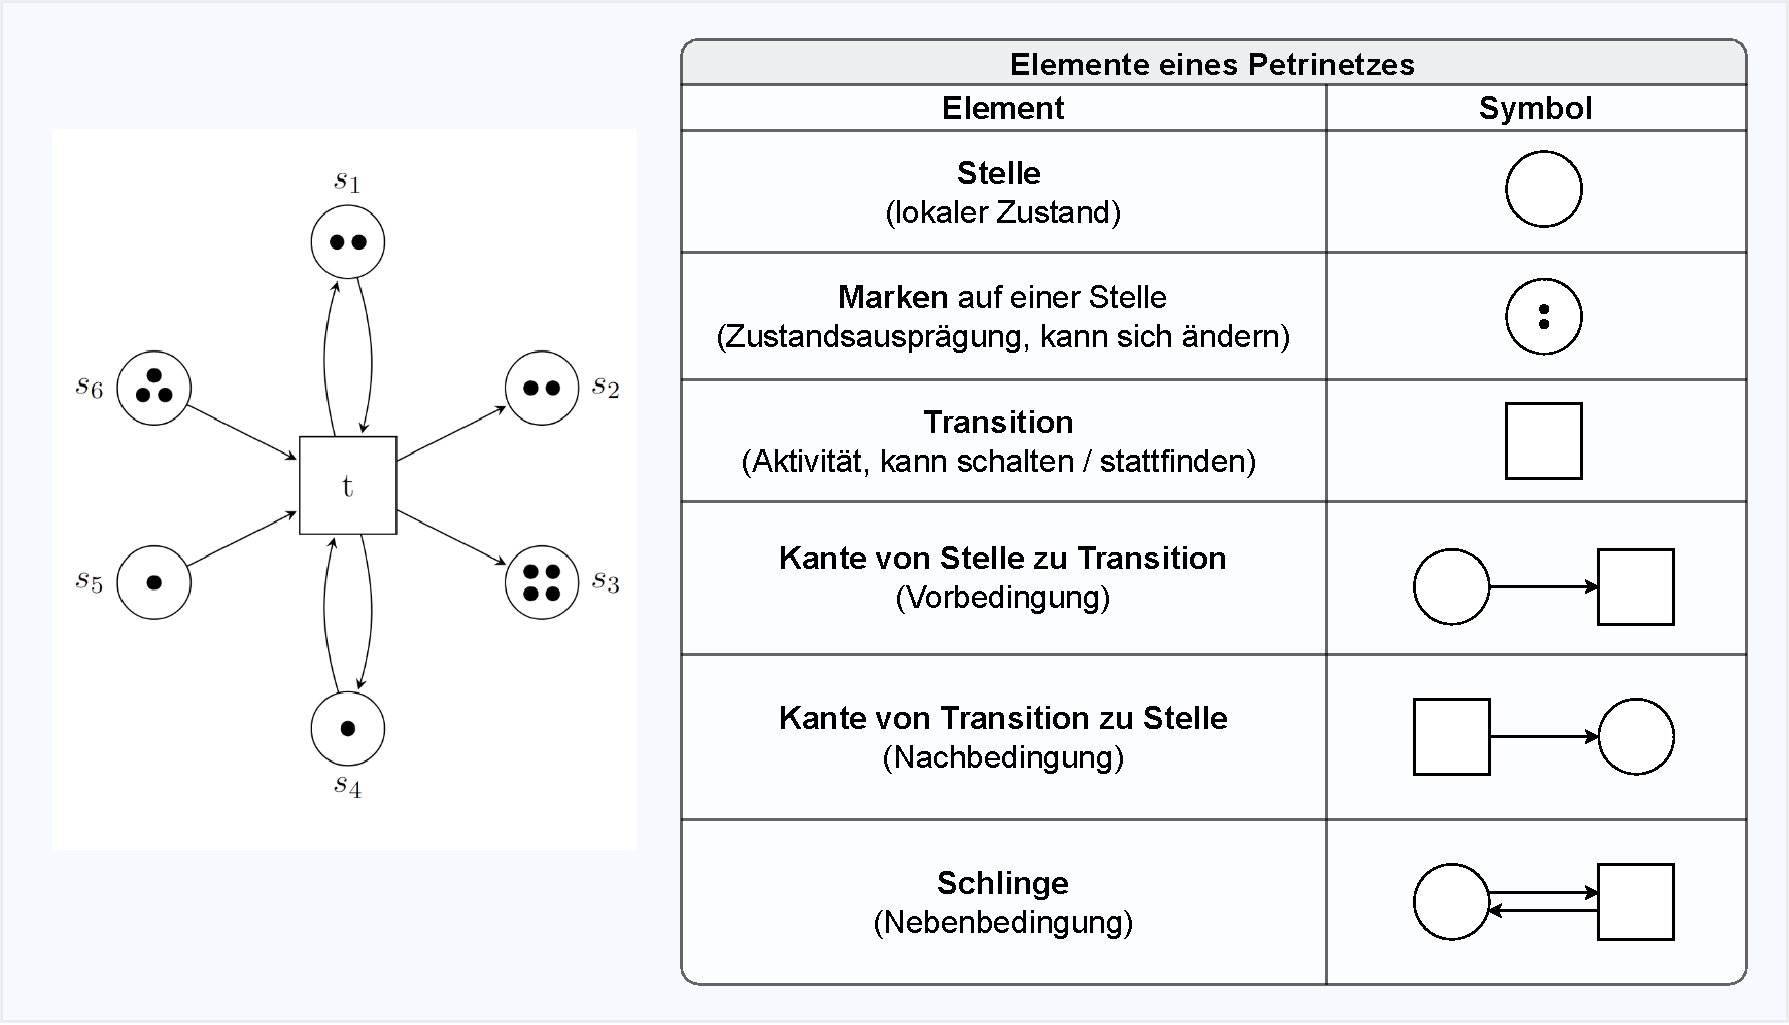
\includegraphics[width=\linewidth]{Bilder/Kapitel-5/grundelemente_petrinetze.pdf}
		\caption{Elemente von Petrinetzen}
		\label{fig:grundelemente_petrinetze}
	\end{addmargin*}
	\end{addmargin*}
\end{figure}

\minisec{Stellen}

Sie haben Stellen bereits in Petrinetzen kennengelernt, die Abläufe modellieren. 
\marginline{Stellen in Ablaufmodellen}
Dort repräsentieren sie Bedingungen, die unmittelbare kausale Abhängigkeiten von Aktionen darstellen. Jede derartige Bedingung kann unerfüllt oder erfüllt sein und gehört (mit Ausnahme von Anfang und Ende) stets zu einer Transition, nach deren Schalten sie erfüllt ist und zu einer Transition, deren Voraussetzung sie ist.

Nutzt man Petrinetze als Systemmodelle, können Stellen viel mehr ausdrücken. 
\marginline{Stellen im Systemmodell}
Es können mehrere Kanten zu einer Stelle führen, und es können mehrere Kanten von einer Stelle ausgehen und dadurch Alternativen dargestellt werden. Zudem kann eine Stelle auch mehr als nur zwei mögliche Zustände (unmarkiert / markiert bzw. unerfüllte Bedingung / erfüllte Bedingung) haben, denn sie kann auch mehr als eine Marke tragen. Dies kommt zwar in den meisten Modellen nur selten vor, aber ist zur Modellierung von mehrfach vorhandenen Ressourcen nützlich. Oder auch einfach dafür, denkbare Fehlerfälle (zum Beispiel unerwünschtes Überschreiben einer Variable oder Überlaufszenarien) formulieren zu können, auch wenn diese bei Modellen korrekter Systeme nicht vorkommen.


\minisec{Markierungen}

Um Verhalten eines Petrinetzes zu modellieren, benötigen wir Markierungen. Anschaulich ist eine Markierung eine Verteilung von Marken auf Stellen. Formal ist eine Markierung definiert als eine Abbildung $m: S \rightarrow \mathbb{N}_0$, die jeder Stelle $ s $ aus der Stellenmenge $S$ die natürliche Zahl $ m(s) $ zuweist. Diese Zahl $ m(s) $ gibt an, wie viele Marken sich auf der Stelle $ s $ befinden.

Wenn die Stellen (zum Beispiel durch Indizes der Form $ s_1, \ldots, s_k$ oder alphabetisch $A, B, C, \ldots$) geordnet sind, dann kann man eine Markierung $m$ als Vektor

$$ \underline{m} =
\begin{pmatrix}
	a_1 \\ \vdots \\ a_k
\end{pmatrix}
$$

schreiben, wobei $a_i$ die Zahl der Marken auf der $i$-ten Stelle ist.

\begin{figure}[!htbp]
	\centering
	\begin{minipage}[c]{.45\textwidth} 
		\centering
		\scalebox{0.8}{
			\petrinetz{
				% Places
				\node[place, tokens=1,label=left:$s_1$] (place1) at (2,0) {};
				\node[place, tokens=0,label=left:$s_2$] (place2) at (6,-2) {};
				\node[place, tokens=0,label=left:$s_3$] (place3) at (6,2) {};
				
				% Transitions
				\node[transition] (trans1) at (8,0) {};
				\node[transition] (trans2) at (4,0) {};
				
				% Edges
				\draw
				(place1) edge[post, bend left=15] (trans2)
				(place1) edge[pre, bend right=15] (trans2)
				(trans2) edge[post] (place2)
				(place2) edge[post] (trans1)
				(trans1) edge[post] (place3)
				(place3) edge[pre] (trans2);
			}
		}
		\vspace{1em}
		
		\textbf{$m_0$}\\
		~\\
		$m_0(s_1)=1$, $m_0(s_2)=0$, $m_0(s_3)=0$\\
		~\\
		$\underline{m_0}=
		\begin{pmatrix}
			1 \\ 0 \\ 0
		\end{pmatrix}$
	\end{minipage}
	\begin{minipage}[c]{.05\textwidth} 
		\centering
		{\color{FernUni-MI-green}\rule{1pt}{90mm}} % senkrechte farbige Linie
	\end{minipage}
	\begin{minipage}[c]{.45\textwidth}
		\centering
		\scalebox{0.8}{
			\petrinetz{
				% Places
				\node[place, tokens=1,label=left:$s_1$] (place1) at (2,0) {};
				\node[place, tokens=5,label=left:$s_2$](place2) at (6,-2) {};
				\node[place, tokens=7,label=left:$s_3$] (place3) at (6,2) {};
				
				% Transitions
				\node[transition] (trans1) at (8,0) {};
				\node[transition] (trans2) at (4,0) {};
				
				% Edges
				\draw
				(place1) edge[post, bend left=15] (trans2)
				(place1) edge[pre, bend right=15] (trans2)
				(trans2) edge[post] (place2)
				(place2) edge[post] (trans1)
				(trans1) edge[post] (place3)
				(place3) edge[pre] (trans2);
			}
		}
		\vspace{1em}
		
		\textbf{$m_7$}\\
		~\\
		$m_7(s_1)=1$, $m_7(s_2)=5$, $m_7(s_3)=7$\\
		~\\
		$\underline{m_7}=
		\begin{pmatrix}
			1 \\ 5 \\ 7
		\end{pmatrix}$
	\end{minipage}
	\caption{Beispiele für Markierungen}
	\label{fig:}
\end{figure}


Markierungen modellieren globale Zustände, konstituiert aus den lokalen Zuständen der einzelnen Stellen.

\minisec{Transitionen}

Wenn ein Petrinetz ein System darstellt, 
\marginline{Transitionen in Ablauf- und Systemmodellen}
dann modellieren Transitionen Aktivitäten. Wird ein Petrinetz zur Beschreibung eines Ablaufs verwendet, dann modellieren Transitionen Aktionen; die zugehörigen Aktivitäten bzw. die Transitionen eines System\-modells findet man dann meist als Label.


\minisec{Kanten und Markenspiel}

Bevor die Semantik, also die Schaltregel, in einer späteren Vorlesung formal definiert wird, sei hier für kleine Beispiele ein Spezialfall angegeben:

Wir betrachten ein Petrinetz $N=(S,T,F)$. 
\sttpkapitelverweis{Vorgriff Schaltregel (Definition~5.9)}{S.~\pageref{text:schaltregel}}
Eine Transition $t$ kann schalten, wenn jede Stelle $s$ mit $(s,t) \in F$ (wenigstens) eine Marke trägt. Wenn $t$ schaltet, wird von jeder dieser Stellen eine Marke entfernt und auf jeder Stelle $s$ mit $(t,s) \in F$ eine Marke hinzufügt, sodass immer wieder neue Markierungen erreicht werden. In einfachen Fällen entsteht dadurch ein "`Markenfluss"', der oft dem Kontrollfluss des modellierten Systems entspricht.


\subsection*{Deterministische Petrinetze}

Jede erreichbare Markierung kann keine, eine oder mehrere Transitionen aktivieren. Durch das Schalten einer Transition können neue Transitionen aktiviert werden. Es kann aber auch sein, dass eine andere, zuvor aktivierte Transition danach nicht mehr aktiviert ist, wenn nämlich eine von ihr benötigte Marke konsumiert wurde. Dieser Fall wird bezeichnet als 
\begin{itemize}
	\item Auswahl (zu welcher Transition geht die Marke?),
	\item Konflikt (zwei Transitionen „streiten“ um die Marke) oder
	\item Nichtdeterminismus (verschiedene Fortsetzungen sind möglich, es wurde keine spezifiert).
\end{itemize}

\begin{figure}[!htbp]
	\centering
	\scalebox{0.6}{
		\petrinetz{
			\draw[colDummyLine](-1,0) -- (19,0);
			
			% Places
			\node[place, tokens=0, label=left:$B$]  (place1) at (1.5,2.6) {}; 
			\node[place, tokens=1, label=below:$A$] (place2) at (1.5,-2.6) {}; 
			\node[place, tokens=0, label=right:$C$] (place3) at (6,0) {}; 
			\node[place, tokens=0, label=left:$G$]  (place4) at (12,0) {}; 
			\node[place, tokens=0, label=above:$F$] (place5) at (16.5,2.6) {}; 
			\node[place, tokens=1, label=below:$E$] (place6) at (16.5,-2.6) {}; 
			\node[place, tokens=0, label=above:$D$] (place7) at (9,2.6) {}; 
			\node[place, tokens=0, label=below:$H$] (place8) at (9,-2.6) {};
			
			% Transitions
			\node[transition, label=left:$a$]  (trans1) at (0,0) {}; 
			\node[transition, label=above:$b$] (trans2) at (4.5,2.6) {}; 
			\node[transition, label=below:$c$] (trans3) at (4.5,-2.6) {}; 
			\node[transition, label=above:$e$] (trans4) at (13.5,2.6) {}; 
			\node[transition, label=below:$f$] (trans5) at (13.5,-2.6) {}; 
			\node[transition, label=right:$d$] (trans6) at (18,0) {};
			
			
			% Kanten
			\draw (trans1) edge[post, bend left=20] (place1) (place1) edge[post, bend left=20] (trans2) (trans2) edge[post, bend left=20] (place3) (place3) edge[post, bend left=20] (trans3) (trans3) edge[post, bend left=20] (place2) (place2) edge[post, bend left=20] (trans1) (trans2) edge[post] (place7) (place7) edge[post] (trans4) (trans5) edge[post] (place8) (place8) edge[post] (trans3) (trans4) edge[post, bend right=20] (place4) (place4) edge[post, bend right=20] (trans5) (trans5) edge[post, bend right=20] (place6) (place6) edge[post, bend right=20] (trans6) (trans6) edge[post, bend right=20] (place5) (place5) edge[post, bend right=20] (trans4);
		}
	}
	\caption{Ein deterministisches Petrinetz}
	\label{fig:v3-deterministisches_Petrinetz}
\end{figure}

Bei deterministischen Petrinetzen kommt Nichtdeterminismus nicht vor. Typischerweise haben deterministische Petrinetze keine Stellen mit mehreren ausgehenden Kanten -- jede Marke kann dann nur von höchstens einer Transition konsumiert werden.

Vorsicht! Determinismus bedeutet nicht, dass die Anfangsmarkierung bzw.\ dass jede erreichbare Markierung nur eine Transition aktiviert. Die Markierung in Abbildung~\ref{fig:v3-deterministisches_Petrinetz} aktiviert beispielsweise die Transitionen $a$ und $d$. Es gibt aber trotzdem nur einen Ablauf (der aber mehrere sequentielle Beobachtungen hat). In anderen Worten: Aktiviert in deterministischen Petrinetzen eine Markierung mehrere Transitionen, so sind diese \textbf{nebenläufig} aktiviert.

\pagebreak %%% für Druck

\subsection*{Nicht-deterministische Petrinetze}	

In einem nicht-determinstischen Petrinetz gibt es Transitionen, die durch Marken auf derselben Stelle aktiviert werden. Abbildung~\ref{fig:v3-nicht-deterministisches Petrinetz} zeigt ein solches Netz: Nach Schalten von $a$ und $d$ (nebenläufig) stehen die Transitionen $b$ und $e$ in Konflikt. Es kann nur eine der beiden Transitionen ausgeführt werden, während die andere dadurch deaktiviert wird.

\begin{figure}[!htbp]
	\centering
	\scalebox{0.6}{
		\petrinetz{
			\draw[colDummyLine](-1,0) -- (19,0); 
			
			% Places
			\node[place, tokens=0, label=left:$B$]  (place1) at (1.5,2.6) {}; 
			\node[place, tokens=1, label=below:$A$] (place2) at (1.5,-2.6) {}; 
			\node[place, tokens=0, label=right:$C$] (place3) at (6,0) {}; 
			\node[place, tokens=0, label=left:$G$]  (place4) at (12,0) {}; 
			\node[place, tokens=0, label=above:$F$] (place5) at (16.5,2.6) {}; 
			\node[place, tokens=1, label=below:$E$] (place6) at (16.5,-2.6) {}; 
			\node[place, tokens=1, label=above:$D$] (place7) at (9,0) {};
			%\node[place, tokens=1, label=below:$H$] (place8) at (8,-2.6) {};
			
			% Transitions
			\node[transition,label=left:$a$]   (trans1) at (0,0) {}; 
			\node[transition, label=above:$b$] (trans2) at (4.5,2.6) {}; 
			\node[transition, label=below:$c$] (trans3) at (4.5,-2.6) {}; 
			\node[transition, label=above:$e$] (trans4) at (13.5,2.6) {}; 
			\node[transition, label=below:$f$] (trans5) at (13.5,-2.6) {}; 
			\node[transition, label=right:$d$] (trans6) at (18,0) {};
			
			% Kanten
			\draw (trans1) edge[post, bend left=20] (place1) (place1) edge[post, bend left=20] (trans2) (trans2) edge[post, bend left=20] (place3) (place3) edge[post, bend left=20] (trans3) (trans3) edge[post, bend left=20] (place2) (place2) edge[post, bend left=20] (trans1) (trans2) edge[pre] (place7) (place7) edge[post] (trans4) (trans5) edge[post] (place7) (place7) edge[pre] (trans3) (trans4) edge[post, bend right=20] (place4) (place4) edge[post, bend right=20] (trans5) (trans5) edge[post, bend right=20] (place6) (place6) edge[post, bend right=20] (trans6) (trans6) edge[post, bend right=20] (place5) (place5) edge[post, bend right=20] (trans4);
		}
	}
	\caption{Nicht-deterministisches Petrinetz}
	\label{fig:v3-nicht-deterministisches Petrinetz}
\end{figure}


\subsection*{Komponenten und Lokalität}	

Abbildung~\ref{fig:v3-Komponenten-und-lokalitaet} zeigt mögliche Komponenten des Petrinetzes aus Abbildung~\ref{fig:v3-deterministisches_Petrinetz} (blaue Kreise). Elemente innerhalb derselben Komponente sind \textbf{lokal}. Beispiel: Transition $a$ und Stelle $C$ befinden sich in derselben Lokalität (obwohl sie nicht direkt mit einer Kante verbunden sind). Verbindungen zwischen Elementen aus unterschied\-lichen Komponenten können als \textbf{global} angesehen werden.

\begin{figure}[!htbp]
	\centering
	\scalebox{0.6}{
		\petrinetz{ 
			\draw[colDummyLine](-1,0) -- (19,0); 
			
			\fill[teal!70!blue, opacity=0.2] (3,0) circle (4); 
			\fill[teal!70!blue, opacity=0.2] (9,2.6) circle (1); 
			\fill[teal!70!blue, opacity=0.2] (9,-2.6) circle (1); 
			\fill[teal!70!blue, opacity=0.2] (15,0) circle (4);
			
			% Places
			\node[place, tokens=0, label=left:$B$]  (place1) at (1.5,2.6) {}; 
			\node[place, tokens=1, label=below:$A$] (place2) at (1.5,-2.6) {}; 
			\node[place, tokens=0, label=right:$C$] (place3) at (6,0) {}; 
			\node[place, tokens=0, label=left:$G$]  (place4) at (12,0) {}; 
			\node[place, tokens=0, label=above:$F$] (place5) at (16.5,2.6) {}; 
			\node[place, tokens=1, label=below:$E$] (place6) at (16.5,-2.6) {}; 
			\node[place, tokens=0, label=above:$D$] (place7) at (9,2.6) {}; 
			\node[place, tokens=0, label=below:$H$] (place8) at (9,-2.6) {};
			
			% Transitions
			\node[transition, label=left:$a$]  (trans1) at (0,0) {}; 
			\node[transition, label=above:$b$] (trans2) at (4.5,2.6) {}; 
			\node[transition, label=below:$c$] (trans3) at (4.5,-2.6) {}; 
			\node[transition, label=above:$e$] (trans4) at (13.5,2.6) {}; 
			\node[transition, label=below:$f$] (trans5) at (13.5,-2.6) {}; 
			\node[transition, label=right:$d$] (trans6) at (18,0) {};
			
			% Kanten
			\draw (trans1) edge[post, bend left=20] (place1) (place1) edge[post, bend left=20] (trans2) (trans2) edge[post, bend left=20] (place3) (place3) edge[post, bend left=20] (trans3) (trans3) edge[post, bend left=20] (place2) (place2) edge[post, bend left=20] (trans1) (trans2) edge[post] (place7) (place7) edge[post] (trans4) (trans5) edge[post] (place8) (place8) edge[post] (trans3) (trans4) edge[post, bend right=20] (place4) (place4) edge[post, bend right=20] (trans5) (trans5) edge[post, bend right=20] (place6) (place6) edge[post, bend right=20] (trans6) (trans6) edge[post, bend right=20] (place5) (place5) edge[post, bend right=20] (trans4);
		}
	}
	\caption{Komponenten und Lokalität}
	\label{fig:v3-Komponenten-und-lokalitaet}
\end{figure}

\clearpage
\section{Vorlesung 4: Eigenschaften von Petrinetzen}

Wir beginnen diese Vorlesung mit der vollständigen Definition von Petrinetzen, die auch Kantengewichte berücksichtigt.

\vspace{-0.3cm} %%% für Druck

\sttpDefinitionskasten{\sttpDefinitionskastenSkalierungsfaktorKapPN}{Definition 5.8: Petrinetz}{}{Ein \textbf{Petrinetz} ist ein Tupel $(S, T, F, m_0)$ mit
	\begin{itemize}
		\item $S$ -- Menge der Stellen, endlich
		\item $T$ -- Menge der Transitionen, endlich, $S \cap T = \emptyset$
		\item $F$ -- Flussrelation, $F \subseteq (S \times T) \cup (T \times S)$
		\item $m_0$ -- Anfangsmarkierung, $m_0 : S \to \{0, 1, 2, \dots\}$
		\item $w$ -- Kantengewichte, $w: F \to \{1, 2, 3, \dots\}$
	\end{itemize}
	Ein Kantengewicht spezifiziert, wie viele Marken beim Schalten der Transition von der Stelle konsumiert bzw. produziert werden.
}

\vspace{-0,8cm} %%% für Druck

\phantomsection
\label{text:schaltregel}	
\sttpDefinitionskasten{\sttpDefinitionskastenSkalierungsfaktorKapPN}{Definition 5.9: Schaltregel}{}{
	Eine Transition $ t $ ist \textit{aktiviert} durch eine Markierung $m$ wenn
	\[
	(s,t) \in F \implies w(s,t) \leq m(s)
	\]
	
	Die Nachfolgemarkierung $m'$ wird nach Schalten von $t$ erreicht:
	\[
	m'(s) =
	\begin{cases}
		m(s) & \text{für } (s,t) \notin F \text{ und } (t,s) \notin F \\
		m(s) - w(s,t) & \text{für } (s,t) \in F \text{ und } (t,s) \notin F \\
		m(s) + w(t,s) & \text{für } (s,t) \notin F \text{ und } (t,s) \in F \\
		m(s) - w(s,t) + w(t,s) & \text{für } (s,t) \in F \text{ und } (t,s) \in F \\
	\end{cases}
	\]
	Eine von einer Markierung $m_1$ aktivierte
	\emph{Schaltfolge} wird definiert als eine Folge von Transitionen $t_1 \; t_2 \; t_3
	\ldots t_n$ so dass \[m_1 \xrightarrow{t_1} m_2 \xrightarrow{t_2} m_3
	\xrightarrow{t_3} \ldots \xrightarrow{t_{n}} m_{n+1},\] wobei die in einer Schaltfolge auftretenden $t_i$
	nicht alle unterschiedlich sein müssen.\\
	Unendliche Schaltfolgen sind entsprechend definiert, und sie führen natur\-ge\-mäß nicht zu einer Markierung.
}

Die Schaltregel definiert, 
\marginline{Aktivierungs\-bedingung und Auswirkung}
wann eine Transition schalten kann und wie sich ihr Schalten auswirkt. Beides ist nur von der Markierung der Stellen abhängig, mit denen die Transition unmittelbar verbunden ist. Dies wird in einem dazugehörigen \mbox{Ablaufnetz} deutlich: die entsprechende Aktion wird auch dort durch eine Transition modelliert, deren umgebende Stellen mit den umgebenden Stellen im Systemnetz übereinstimmen.

Formal definiert ist die Schaltregel für eine Markierung, also dem Modell eines globalen Zustands, und es entsteht eine neue Markierung. Von dieser aus kann wieder eine Transition schalten usw., wir erhalten eine Folge nacheinander möglicher Schaltvorgänge, die bei einer endlichen Schaltfolge wieder zu einer Markierung führen.

Schaltfolgen 
\marginline{Schaltfolge}
beschreiben wie die Linearisierungen der halbgeordneten Abläufe eine sequentielle Sicht der Abläufe. Tatsächlich stimmen diese Sequenzen überein, wie das folgende Theorem zeigt:

\sttpTheorem{\sttpTheoremSkalierungsfaktor}{Die Menge der sequentiellen Beobachtungen von Ablaufnetzen eines Petrinetzes ist gleich der Menge der von der Anfangsmarkierung aktivierten Schaltfolgen.}

Wir interessieren uns im Folgenden für durch Schaltfolgen erreichte und erreichbare Markierungen sowie die durch sie aktivierten Transitionen. Es wurde nicht formal definiert, welche Markierung durch einen Ablauf erreicht wird. Sie stimmt überein mit der durch eine beliebige Linearisierung erreichten Markierung und deshalb auch mit der Markierung, die durch die entsprechende Schaltfolge erreicht wird.

\subsection*{Zustandsgraph}

An einem Zustandsgraph (auch Erreichbarkeitsgraph) kann man die erreichbaren Markierungen und Schaltfolgen eines Netzes ablesen. Das ist hilfreich bei Erreichbarkeitsanalysen.

%%% Für den Druck wurde die Aufzählung vor die Grafik verschoben ...

\begin{itemize}
	\item Die Knoten des Zustandsgraphen entsprechen den erreichbaren Markierungen des Petrinetzes. Jeder Knoten gibt an, wie viele Marken sich auf den einzelnen Stellen befinden.
	\item Der Anfangsknoten repräsentiert die Anfangsmarkierung $m_0$, die initiale Verteilung der Marken im Petrinetz. Dieser Knoten wird gekennzeichnet durch einen Pfeil, der auf den Knoten zeigt.
	\item Jede Kante zwischen zwei Knoten im Zustandsgraph steht für einen Übergang von einer Markierung zu einer anderen durch das Schalten derjenigen Transition, mit der die Kante beschriftet ist.
\end{itemize}

\begin{figure}[h!]
	\centering
	\begin{minipage}[c]{.45\textwidth} 
		\centering
		\scalebox{0.8}{
			\petrinetz{
				\draw[colDummyLine](0, 0.9) -- (0, -2.8);
				
				% Places
				\node[place, tokens=1, label=below:$s_1$] (place1) at (0,-2) {};
				\node[place, tokens=1, label=above:$s_2$] (place2) at (2,0) {};
				\node[place, tokens=0, label=below:$s_3$] (place3) at (4,-2) {};
	
				% Transitions
				\node[transition, label=above:$t_1$] (trans1) at (0,0) {};
				\node[transition, label=below:$t_3$] (trans3) at (2,-2) {};
				\node[transition, label=above:$t_2$] (trans2) at (4,0) {};
				
				% Edges
				\draw
					(trans1) edge[post] (place2)
					(place2) edge[post] (trans2)
					(trans2) edge[post] (place3)
					(place3) edge[post] (trans3)
					(trans3) edge[post] node[midway, right] {2} (place2)
					(place1) edge[post] (trans3)
					(place1) edge[post] (trans1)
				;
			}
		}
%		%%% für den Druck keine weiteren Bildunterschriften
%		Petrinetz zum Zustandsgraph
	\end{minipage}
	\begin{minipage}[c]{.05\textwidth} 
		\centering
		{\color{FernUni-MI-green}\rule{1pt}{30mm}} % senkrechte farbige Linie
	\end{minipage}
	\begin{minipage}[c]{.45\textwidth}
		\centering
		\scalebox{0.8}{
			\petrinetz{
				\tikzset{
					node style/.style={draw, circle, fill=blue!50!black, minimum size=3pt, inner sep=0pt}
				}
				
				\draw[colDummyLine](0, 0.9) -- (0, -2.8);
	
				% Bommel mit Labels
				\node[node style, label={above:(110)}] (m0) at (0,0){};
				\node[node style, label={above:(101)}] (m1) at (2,0) {};
				\node[node style, label={below:(020)}] (m2) at (0,-2) {};
				\node[node style, label={below:(011)}] (m3) at (2,-2) {};
				\node[node style, label={below:(002)}] (m4) at (4,-2) {}; 
				
				\draw[->] (-1,0) -- (0,0);
				\draw[->] (m0) -- (m1) node[midway, above] {$t_2$};
				\draw[->] (m0) -- (m2) node[midway, left] {$t_1$};
				\draw[->] (m1) -- (m2) node[midway, left] {$t_3$};
				\draw[->] (m1) -- (m3) node[midway, right] {$t_1$};
				\draw[->] (m2) -- (m3) node[midway, below] {$t_2$};
				\draw[->] (m3) -- (m4)node[midway, below] {$t_2$};
			}
		}
%		%%% für den Druck keine weiteren Bildunterschriften
%		Zustandsgraph zum Petrinetz
	\end{minipage}
	\caption{Petrinetz und Zustandsgraph}
	\label{fig:petrinetz_und_zustandsgraph}
\end{figure}


Abbildung~\ref{fig:petrinetz_und_zustandsgraph} zeigt ein Petrinetz und den zugehörigen Zustandsgraph. Insbesondere wird sichtbar, dass insgesamt fünf Markierungen (inklusive der Anfangsmarkierung) erreichbar sind.

Schaltfolgen des Petrinetzes sind an den gerichteten Pfaden des Zustandsgraphen abzulesen. So gibt es z.B. einen Pfad, dessen Kanten beschriftet sind mit $t_2$, $t_3$, $t_2$, $t_2$ und dies ist auch eine Schaltfolge des Netzes. Tatsächlich existiert für jede Schaltfolge ein entsprechender Pfad und umgekehrt.

\subsection*{Eigenschaften von Petrinetzen}

Mit Schaltfolgen und Markierungen kann man eine Reihe wichtiger Eigenschaften von Petrinetzen einfach formal definieren:

Ein Petrinetz ist

\begin{itemize}
	\item \textbf{terminierend}, wenn es keine unendlichen Schaltfolgen gibt,
	\item \textbf{Deadlock-frei}, wenn jede erreichbare Markierung mindestens eine Transition aktiviert,
	\item \textbf{lebendig}, wenn jede erreichbare Markierung eine Schaltfolge aktiviert, in der jede Transition vorkommt,
	\item \textbf{b-beschränkt}, wenn für jede erreichbare Markierung $m$ und jede Stelle $s$ gilt: $m(s) \leq b$,
	\item \textbf{beschränkt}, wenn es $b$-beschränkt ist für irgendeine Schranke $b$,
	\item \textbf{sicher}, wenn es 1-beschränkt ist,
	\item \textbf{reversibel}, wenn $m_0$ von jeder erreichbaren Markierung aus erreichbar ist.
\end{itemize}


\phantomsection
\label{text:zentrale_eigenschaften_zustandsgraph}
Diese Eigenschaften 
\marginline{zentrale Eigen\-schaften am Zustands\-graph ablesen}
lassen sich mehr oder weniger einfach am Zustandsgraph ablesen:

\begin{itemize}
	\item Eine Markierung ist \textbf{erreichbar} genau dann, wenn sie im Zustandsgraph als Knoten vorkommt.
	\item Ein Petrinetz ist \textbf{terminierend} genau dann, wenn der Zustandsgraph endlich ist und keine Zyklen hat.
	\item Ein Petrinetz ist \textbf{Deadlock-frei} genau dann, wenn jeder Knoten des Zustandsgraph wenigstens einen Nachfolger hat.
	\item Ein Petrinetz ist \textbf{lebendig} genau dann, wenn es von jedem Knoten des Zustandsgraph aus einen Pfad mit allen Transitionen als Label gibt.
	\item Ein Petrinetz ist \textbf{beschränkt} genau dann, wenn der Zustandsgraph endlich viele Knoten enthält (siehe folgendes Theorem).
	\item Ein Petrinetz ist \textbf{reversibel} genau dann, wenn der Zustandsgraph stark 
	\linebreak %%% für Druck
	zusammenhängend ist (s.~Vorlesung~6).
\end{itemize}

Das Petrinetz aus Abbildung~\ref{fig:petrinetz_und_zustandsgraph} ist beschränkt und terminierend, also insbesondere nicht Deadlock-frei, geschweige denn lebendig. Es ist auch nicht reversibel.

\pagebreak %%% für Druck

Das folgende Theorem fasst wichtige Bezüge zwischen den Eigenschaften zusammen:

\sttpTheorem{\sttpTheoremSkalierungsfaktor}{
	\begin{enumerate}
		\item[a)] Jedes terminierende Petrinetz ist nicht Deadlock-frei. Die umgekehrte Richtung gilt nicht.
		\item[b)] Jedes lebendige Petrinetz mit wenigstens einer Transition ist Deadlock-frei.
		\item[c)] Ein Petrinetz ist genau dann lebendig, wenn für jede Transi\-tion $t$ und jede erreichbare Markierung $m$ gilt: $m$ aktiviert eine Schaltfolge zu einer Markierung $m'$, die $t$ aktiviert.
		\item[d)] Jedes beschränkte Petrinetz hat endlich viele erreichbare Markierungen und umgekehrt.
	\end{enumerate}
}

\textbf{Beweis}

\begin{enumerate}
	\item[a)] Wenn ein Netz terminierend ist, führt jede Schaltfolge notwendigerweise zu einem Deadlock. Insbesondere existiert damit ein Deadlock und das Netz ist nicht Deadlock-frei. Die umgekehrte Richtung gilt nicht, denn ein Petrinetz kann sowohl unendliche als auch endliche Schaltfolgen besitzen, die zu einem Deadlock führen.
	
	\item[b)] Jede erreichbare Markierung eines lebendigen Netzes ermöglicht eine Schalt\-folge, in der alle Transitionen schalten können. Insbesondere wird dabei die erste Transition der Schaltfolge aktiviert, sodass kein Deadlock auftreten kann.
	
	\item[c)] Diesen Beweis sollen Sie in einer Einsendeaufgabe selbst finden.
	
	\item[d)] Bei derartigen Äquivalenzaussagen müssen wir beide Richtung getrennt betrachten:
	\begin{enumerate}
		\item[$\Rightarrow$] Wenn das Netz beschränkt ist, dann ist es auch $b$-beschränkt für ein $b$. \linebreak
		Jede Stelle kann daher auf höchstens $b+1$ Weisen markiert werden. Da die Stellenmenge $S$ beschränkt ist, können höchstens ${(b+1)}^{|S|}$ Markierungen erreicht werden. Insbesondere ist also die Menge erreichbarer Markierungen endlich.
		\item[$\Leftarrow$] In einer endlichen Menge von Markierungen existiert ein maximaler Wert, der durch eine der Markierungen einer Stelle zugewiesen wird. Dieser Wert ist eine geeignete Schranke.
	\end{enumerate}
\end{enumerate}

\clearpage
\section{Vorlesung 5: Analyse von Petrinetzen}

Nachdem verschiedene Eigenschaften von Petrinetzen definiert wurden, geht es jetzt zur Analyse von Petrinetzen. Es geht um die Frage, ob ein gegebenes Netz eine Eigenschaft hat oder nicht.

Für beschränkte Petrinetze gelingt die Analyse zuverlässig 
\sttpkapitelverweis{}{S.~\pageref{text:zentrale_eigenschaften_zustandsgraph}}
durch Konstruktion und Analyse des Zustandsgraph (der allerdings sehr groß werden kann). 
Bei einem unbeschränktem Petrinetz ist die Analyse seiner Eigenschaften oft kniffliger. Interessant ist z.B die Frage, ob ...
\begin{itemize}
	\item \textbf{... eine Markierung erreichbar ist.} Das Problem der Erreichbarkeit ist sehr komplex und in seiner allgemeinen Form nicht einfach zu lösen (obwohl es theoretisch entscheidbar ist).
	\item \textbf{... das Netz lebendig ist.} Dies ist ebenfalls ein sehr komplexes, aber entscheidbares Problem.
	\item \textbf{... das Netz beschränkt ist.} 
	\marginline{Unbeschränkt\-heit bestimmen}
	Die Beschränktheit eines Petrinetzes lässt sich während der Konstruktion des Zustandsgraph erkennen. Das Netz ist unbeschränkt, wenn der Zustandsgraph unendlich groß ist, aber man kann genau dies nach Konstruktion eines endlichen Teils entdecken.
\end{itemize}

Wie findet man also heraus, ob ein Netz (un)beschränkt ist? Die Petrinetz-Theorie bietet viele effiziente Verfahren, die wenigstens hinreichende Bedingungen für Beschränktheit prüfen. In folgenden Vorlesungen werden Sie einige davon kennenlernen. Im allgemeinen Fall aber kommen wir um die Konstruktion des Zustandsgraph bzw. eines sehr großen, aber endlichen Teil des Zustandsgraph nicht herum. Das folgende Theorem formuliert eine Eigenschaft unbeschränkter Netze, die bei der Konstruktion des Zustandsgraph eines unbeschränkten Netzes irgendwann entdeckt wird.

\sttpTheorem{\sttpTheoremSkalierungsfaktor}{
	Ein Petrinetz ist unbeschränkt genau dann, wenn es eine von $m_0$ erreichbare Markierung $m$ und eine von $m$ erreichbare Markierung $m'$ gibt, sodass gilt:
	\begin{addmargin}[25pt]{25pt}
		Für jede Stelle $s$ gilt: $m'(s) \geq m(s)$, und für wenigstens eine Stelle $s$ gilt: $m'(s) > m(s)$.
	\end{addmargin}
}

\textbf{Beweis}

Eine Richtung des Beweises ist sehr einfach: Wenn es wie in der Aussage beschriebene Markierungen $m$ und $m'$ gibt, dann kann die Schaltfolge von $m$ nach $m'$ von $m$ aus auch beliebig oft stattfinden, und die Markenzahl auf $s$ erhöht sich über alle Schranken hinweg. Das Petrinetz ist dann also unbeschränkt.

Die umgekehrte Richtung ist nicht so einfach. Für einen formalen Beweis benötigt man Dickson's Lemma\footnote{
	Dickson's Lemma besagt, dass jede nichtleere Teilmenge $T \subseteq \mathbb{N}^r$ (wobei $r$ eine natürliche Zahl ist) bezüglich der komponentenweisen Ordnung nur endlich viele minimale Elemente besitzt. Die komponentenweise Ordnung auf $\mathbb{N}^r$ bedeutet, dass für zwei Elemente $(a_1, a_2, \dots, a_r)$ und $(b_1, b_2, \dots, b_r)$ gilt: 
	$(a_1, a_2, \dots, a_r) \leq (b_1, b_2, \dots, b_r)$ genau dann, wenn $a_i \leq b_i$ für alle $i = 1, 2, \dots, r$.
	}, 
deshalb soll hier nur die Idee skizziert werden. 

\clearpage %%% für Druck

Der Beweis ist nicht prüfungsrelevant.

Da die Menge $T$ der Transitionen endlich ist, existieren höchstens $|T|$ Schaltfolgen der Länge 1, höchstens $|T|^2$ Schaltfolgen der Länge 2, und allgemein höchstens $|T|^n$ Schaltfolgen der Länge $n$. Weil jede erreichbare Markierung durch eine Schaltfolge erreicht wird, können unendlich viele Markierungen nur erreicht werden, wenn es auch wenigstens eine unendliche Schaltfolge gibt, in der auch unendlich viele unterschiedliche Markierungen erreicht werden (werden nur endlich viele Markierungen in einer unendlichen Schaltfolge erreicht, dann unterscheidet diese sich diesbezüglich nicht von ihrem endlichen Anfangsstück, in dem alle in ihr überhaupt erreichten Markierungen bereits vorkommen).

Betrachten wir nun also eine unendliche Schaltfolge, in der auch unendlich viele unterschiedliche Markierungen erreicht werden. Sei $m_0 \: m_1 \: m_2 \ldots$ eine Folge von in dieser Schaltfolge (nacheinander, aber nicht notwendigerweise unmittelbar nacheinander) erreichten Markierungen, die sich alle voneinander unterscheiden. Nun nutzen wir aus, dass auch die Stellenmenge endlich ist und betrachten eine beliebige Reihenfolge $s_1, s_2, \ldots , s_n$ der Stellen.

Für $s_1$ existiert ein minimaler Wert $k_1$ von $\{m_0 (s_1), m_1 (s_1), m_2 (s_1,)\ldots\}$ und eine erste Markierung $m_{i^1_1}$ in der Folge $m_0 \: m_1 \: m_2 \ldots$, sodass $m_{i^1_1} (s_1) = k_1$. In der verbleibenden Restfolge $m_{i^1_1+1}, m_{i^1_1+2}, \ldots$ existiert wieder ein minimaler Wert $k_2$ für die Markierung von $s_1$ und es gilt natürlich $k_2 \geq k_1$. Wir wählen  $m_{i^1_2}$ als erste Markierung der Restfolge, für die $m_{i^1_2} (s_1) = k_2$. Diese Prozedur können wir beliebig fortsetzen; also existiert eine unendliche Folge von Markierungen $m_{i^1_1}\; m_{i^1_2} \;m_{i^1_3}\ldots$ mit der Eigenschaft $m_{i^1_1} (s_1) \leq m_{i^1_2}(s_1) \leq  m_{i^1_3} (s_1)\ldots$. Per Konstruktion ist $m_{i^i_1}$ von $m_0$ erreichbar, $m_{i^1_2} $ von $m_{i^1_1} $, $m_{i^1_3} $ von $m_{i^1_2} $ usw.

Auf dieser Folge $m_{i^1_1} \; m_{i^1_2} \; m_{i^1_3}\ldots$ können wir nun dasselbe mit der Stelle $s_2$ anstellen und erhalten somit eine weitere Folge voneinander erreichbarer Markierungen $m_{i^2_1}\; m_{i^2_2}\; m_{i^2_3}\ldots$, für die nun auch für die Stelle $s_2$ gilt $m_{i^2_1} (s_2) \leq m_{i^2_2} (s_2) \leq m_{i^2_3}(s_2)\ldots$ (und natürlich auch noch $m_{i^2_1} (s_1) \leq m_{i^2_2} (s_1) \leq m_{i^2_3}(s_1)\ldots$).

Entsprechend verfahren wir nacheinander für $s_3$, $s_4$ bis zu $s_n$, also für alle Stellen. Dadurch erhalten wir eine unendliche Folge voneinander erreichbarer
Markierungen $m_{i^n_1}\; m_{i^n_2}\; m_{i^n_3}\ldots$, sodass für jede Stelle $s$ gilt $m_{i^n_1} (s) \leq m_{i^n_2} (s) \leq m_{i^n_3}(s)\ldots$. Betrachten wir die ersten beiden Elemente dieser Folge. Es gilt nach Konstruktion: $m_{i^n_1}$ ist von $m_0$ erreichbar, und $m_{i^n_2}$ von $m_{i^n_1}$. Da alle Markierungen in der Ursprungsfolge unterschiedlich sind, gilt dies auch für  $m_{i^n_2}$ und $m_{i^n_1}$. Folglich gilt für wenigstens eine Stelle $s$: $m_{i^n_1} (s) < m_{i^n_2} (s)$, und damit ist mit $m:= m_{i^n_1}$ und $m':= m_{i^n_2}$ bewiesen, was wir beweisen wollten.

\clearpage
\section{Vorlesung 6: Abläufe von Petrinetzen}

In Vorlesung 2 haben Sie gesehen, 
\sttpkapitelverweis{}{S.~\pageref{text:linearisierung_einer_halbordnung}}
dass man durch die Linearisierung eines halbgeordneten Ablaufs auf die sequentiellen Beobachtungen schließen kann, indem allen nicht geordneten Elementen eine eindeutige Reihenfolge zugewiesen wird. In Vorlesung 5 haben wir festgestellt, dass alle Linearisierungen von Abläufen mögliche Schaltfolgen des Petrinetzes sind, und umgekehrt.

Nun ist es auch möglich, Abläufe ausgehend von den Schaltfolgen eines Petri\-netzes zu konstruieren. Das Ziel ist, dass eine Linearisierung des konstruierten Ablaufs der gegebenen Schaltfolge entspricht, die Schaltfolge also eine mögliche sequentielle Beobachtung des Ablaufs darstellt. Das genaue Vorgehen können Sie in der Videovorlesung 6 nachvollziehen.

Grundsätzlich gibt es in deterministischen Netzen \textbf{einen eindeutigen} Ablauf, der durch jede Schaltfolge generiert wird. Interessant sind deshalb nicht-deterministische Netze. Wir werden im Folgenden Beispiele für drei unterschiedliche Möglichkeiten vorstellen:

\begin{itemize}
	\item Zwei unterschiedliche Schaltfolgen führen zu demselben Ablauf. (1)
	\item Eine Schaltfolge führt zu zwei unterschiedlichen Abläufen. (2)
	\item Zwei unterschiedliche Schaltfolgen führen zu zwei unterschiedlichen Abläufen. (3)
\end{itemize}

Im Warenautomat aus Abbildung~\ref{fig:v6-Keksautomat_ados} stehen  $t_4$ und $t_5$ nach Schalten von $t_3$ in Konflikt, und in der linken Komponente des Netzes gibt es drei Marken, die wir im Ablauf unterscheiden müssen.

\begin{figure}[!htbp]
	\centering
	\scalebox{0.8}{
		\petrinetz{ 
			\node[place, tokens=1, label=above: $s_1$] (place1) at (2,2) {}; 
			\node[place, tokens=2, label=below: $s_5$] (place2) at (2,-2) {}; 
			\node[place, tokens=1, label=above: $s_2$] (place3) at (6,2) {}; 
			\node[place, tokens=0, label=below: $s_4$] (place4) at (6,-2) {}; 
			\node[place, tokens=0, label=right: $s_3$] (place5) at (10,0) {}; 
			\node[transition, label=left: $t_1$] (trans1) at (0,0) {}; 
			\node[transition, label=left: $t_2$] (trans2) at (4,0) {}; 
			\node[transition, label=above: $t_3$] (trans3) at (8,2) {}; 
			\node[transition, label=below: $t_5$] (trans4) at (8,0) {};
			\node[transition, label=below: $t_4$] (trans5) at (8,-2) {};
			
			\draw 
			(trans1)edge[post, bend left=30](place1) (trans2)edge[post, bend left=30](place2) (place2)edge[post, bend left=30](trans1) (place1)edge[post, bend left=30](trans2) 
			(place3)edge[pre, bend right=30](trans2) 
			(place3)edge[post](trans3) 
			(trans3)edge[post, bend left=30](place5) 
			(place5)edge[post](trans4) 
			(place5)edge[post, bend left=30](trans5) 
			(place4)edge[pre](trans5) 
			(trans4)edge[post, bend left=30](place3) 
			(place4)edge[post, bend left=30](trans2);
		}
	}
	\caption{Ein Petrinetz (Systemmodell)}
	\label{fig:v6-Keksautomat_ados}
\end{figure}

\clearpage %%% für Druck

Betrachten wir die folgende Schaltfolge: 

$$t_3 \; t_4 \; t_1 \; t_2 \; t_1 \; t_3$$

Abbildung~\ref{fig:v6-Ablauf} oben zeigt einen passenden Ablauf, bei dem $t_5$ nicht schaltet. Die Transition $t_2$ konsumiert die Marke, die in der Anfangsmarkierung auf $s_1$ liegt.

\vspace{1ex}

{ %% Scope beginnen (damit \newlength keine Auswirkung auf den übrigen Text hat)

\newlength{\mywidth}%
\setlength{\mywidth}{\textwidth}%
\addtolength{\mywidth}{\marginparwidth}%

\begin{figure}[!htbp]
	\begin{addmargin*}[0cm]{-\marginparwidth}
		
	\centering
	\resizebox{1.0\mywidth}{!}{
		\petrinetz{
			% Ablauf 1
 			\draw[colDummyLine] (-1,1) rectangle (25,-7);
			
			% Places
			\node[place, tokens=1,label=left:$s_1$] (place1) at (0, 0) {};
			\node[place, tokens=1,label=left:$s_2$] (place2) at (0, -2) {};
			\node[place, tokens=1, label=left:$s_5$] (place3) at (0, -4) {};
			\node[place, tokens=1, label=left:$s_5$] (place4) at (0, -6) {};
			\node[place, label=below:$s_3$] (place5) at (4, -2) {};
			\node[place, label=right:$s_1$] (place6) at (4, -4) {};
			\node[place, label=right:$s_1$] (place7) at (4, -6) {};
			\node[place, label=below:$s_4$] (place8) at (8, -2) {};
			\node[place, label=below:$s_2$] (place9) at (12, -1) {};
			\node[place, label=right:$s_5$] (place10) at (12, -3) {};
			\node[place, label=right:$s_3$] (place11) at (16, -1) {};
			
			% Transitions
			\node[transition, label=center:$t_3$] (trans1) at (2, -2) {};
			\node[transition, label=center:$t_1$] (trans2) at (2, -6) {};
			\node[transition, label=center:$t_1$] (trans3) at (2, -4) {};
			\node[transition, label=center:$t_4$] (trans4) at (6, -2) {};
			\node[transition, label=center:$t_2$] (trans5) at (10, -2) {};
			\node[transition, label=center:$t_3$] (trans6) at (14, -1) {};
			
			% Edges
			\draw[post, bend left=20] (place1) to (trans5);
			\draw (place2) edge[post] (trans1);
			\draw (place3) edge[post] (trans3);
			\draw (place4) edge[post] (trans2);
			\draw (trans1) edge[post] (place5);
			\draw (trans2) edge[post] (place7);
			\draw (trans3) edge[post] (place6);
			\draw (place5) edge[post] (trans4);
			\draw (trans4) edge[post] (place8);
			\draw (place8) edge[post] (trans5);
			\draw (trans5) edge[post] (place9);
			\draw (trans5) edge[post] (place10);
			\draw (place9) edge[post] (trans6);
			\draw (trans6) edge[post] (place11);
		}
	}
	
	\vspace{-2mm}
	{\color{FernUni-MI-green}\rule{0.9\mywidth}{1pt}} % waagerechte farbige Linie
	\vspace{2mm}
	
	\resizebox{1.0\mywidth}{!}{
		\petrinetz{
			% Ablauf 2
 			\draw[colDummyLine] (-1,1) rectangle (25,-7);
			
			% Places
			\node[place, tokens=1,label=left:$s_1$] (place1) at (0, 0) {};
			\node[place, tokens=1,label=left:$s_2$] (place2) at (0, -2) {};
			\node[place, tokens=1, label=left:$s_5$] (place3) at (0, -4) {};
			\node[place, tokens=1, label=left:$s_5$] (place4) at (0, -6) {};
			\node[place, label=below:$s_3$] (place5) at (4, -2) {};
			\node[place, label=right:$s_1$] (place6) at (4, -4) {};
			\node[place, label=right:$s_1$] (place7) at (4, -6) {};
			\node[place, label=below:$s_4$] (place8) at (8, -2) {};
			\node[place, label=below:$s_2$] (place9) at (12, -1) {};
			\node[place, label=right:$s_5$] (place10) at (12, -3) {};
			\node[place, label=right:$s_3$] (place11) at (16, -1) {};
			
			% Transitions
			\node[transition, label=center:$t_3$] (trans1) at (2, -2) {};
			\node[transition, label=center:$t_1$] (trans2) at (2, -6) {};
			\node[transition, label=center:$t_1$] (trans3) at (2, -4) {};
			\node[transition, label=center:$t_4$] (trans4) at (6, -2) {};
			\node[transition, label=center:$t_2$] (trans5) at (10, -2) {};
			\node[transition, label=center:$t_3$] (trans6) at (14, -1) {};
			
			% Edges
			\draw[post] (place7) to (trans5);
			\draw (place2) edge[post] (trans1);
			\draw (place3) edge[post] (trans3);
			\draw (place4) edge[post] (trans2);
			\draw (trans1) edge[post] (place5);
			\draw (trans2) edge[post] (place7);
			\draw (trans3) edge[post] (place6);
			\draw (place5) edge[post] (trans4);
			\draw (trans4) edge[post] (place8);
			\draw (place8) edge[post] (trans5);
			\draw (trans5) edge[post] (place9);
			\draw (trans5) edge[post] (place10);
			\draw (place9) edge[post] (trans6);
			\draw (trans6) edge[post] (place11);
		}
	}

	\vspace{-2mm}
	{\color{FernUni-MI-green}\rule{0.9\mywidth}{1pt}} % waagerechte farbige Linie
	\vspace{2mm}

	\resizebox{1.0\mywidth}{!}{
		\petrinetz{
			% Ablauf 3
 			\draw[colDummyLine] (-1,1) rectangle (25,-7);
			
			% Places
			\node[place, tokens=1,label=left:$s_1$] (place1) at (0, 0) {};
			\node[place, tokens=1,label=left:$s_2$] (place2) at (0, -2) {};
			\node[place, tokens=1, label=left:$s_5$] (place3) at (0, -4) {};
			\node[place, tokens=1, label=left:$s_5$] (place4) at (0, -6) {};
			\node[place, label=below:$s_3$] (place5) at (4, -2) {};
			\node[place, label=right:$s_1$] (place6) at (4, -4) {};
			\node[place, label=below:$s_1$] (place7) at (4, -6) {};
			\node[place, label=below:$s_2$] (place8) at (8, -2) {};
			\node[place, label=below:$s_2$] (place9) at (20, -1) {};
			\node[place, label=right:$s_5$] (place10) at (20, -3) {};
			\node[place, label=right:$s_3$] (place11) at (24, -1) {};
			\node[place, label=below:$s_3$] (place12) at (12, -2) {};
			\node[place, label=above:$s_4$] (place13) at (16, -2) {};
			
			% Transitions
			\node[transition, label=center:$t_3$] (trans1) at (2, -2) {};
			\node[transition, label=center:$t_1$] (trans2) at (2, -6) {};
			\node[transition, label=center:$t_1$] (trans3) at (2, -4) {};
			\node[transition, label=center:$t_5$] (trans4) at (6, -2) {};
			\node[transition, label=center:$t_2$] (trans5) at (18, -2) {};
			\node[transition, label=center:$t_3$] (trans6) at (22, -1) {};
			\node[transition, label=center:$t_3$] (trans7) at (10, -2) {};
			\node[transition, label=center:$t_4$] (trans8) at (14, -2) {};
			
			% Edges
			\draw[post] (place7) to (trans5);
			\draw (place2) edge[post] (trans1);
			\draw (place3) edge[post] (trans3);
			\draw (place4) edge[post] (trans2);
			\draw (trans1) edge[post] (place5);
			\draw (trans2) edge[post] (place7);
			\draw (trans3) edge[post] (place6);
			\draw (place5) edge[post] (trans4);
			\draw (trans4) edge[post] (place8);
			%\draw (place8) edge[post] (trans5);
			\draw (trans5) edge[post] (place9);
			\draw (trans5) edge[post] (place10);
			\draw (place9) edge[post] (trans6);
			\draw (trans6) edge[post] (place11);
			\draw (place8) edge[post] (trans7);
			\draw (trans7) edge[post] (place12);
			\draw (place12) edge[post] (trans8);
			\draw (trans8) edge[post] (place13);
			\draw (place13) edge[post] (trans5);
		}
	}
	\caption{Verschiedene Abläufe zum Systemmodell}
	\label{fig:v6-Ablauf}
	
	\end{addmargin*}
\end{figure}

} %% Scope beenden (um \newlength lokal zu halten)

\clearpage

(1) Derselbe Ablauf kann entstehen, wenn wir mit einer anderen Linearisierung der Halbordnung als Schaltfolge beginnen, also z.B. mit:

$$t_1 \; t_1\; t_3 \; t_4 \; t_2 \; t_3$$

(2) In Abbildung~\ref{fig:v6-Ablauf} Mitte sehen wir einen anderen Ablauf zu derselben Schaltfolge. $t_2$ konsumiert nun eine Marke, die in der Anfangsmarkierung auf $s_5$ liegt und nach einmaligem Schalten von $t_1$ auf $s_1$. Bei der Konstruktion eines Ablaufes haben wir die Wahl, welche mit $s_1$ beschriftete Stelle durch eine Kante mit der neuen Transition verbunden werden soll. Das liegt daran, dass nach den zuvor geschalteten Transitionen mehrere Marken auf $s_1$ liegen. Umgekehrt gilt: Bei 1-beschränkten Netzen tritt dieses Phänomen nicht auf. 

\vspace{\baselineskip}

(3) Dieser dritte mögliche Ablauf -- Sie sehen das Potenzial für unendlich mehr davon -- in Abbildung~\ref{fig:v6-Ablauf} unten ist länger, weil das Schalten von $t_5$ dazu führt, dass $t_4$ erst später schalten kann. Grundlage dieses Ablaufs ist z.B. die Schaltfolge

$$t_3 \; t_5 \; t_1 \; t_3 \; t_1 \; t_4 \; t_2 \;  t_3 $$

Aus der Konstruktionsvorschrift der Abläufe ergibt sich:
\begin{itemize}
	\item Führt im Ablauf eine Kante von einer mit $s$ beschrifteten Stelle zu einer mit $t$ beschrifteten Transition, dann führt auch im Systemnetz eine Kante von $s$ nach $t$. Dasselbe gilt für Kanten von Transitionen zu Stellen.
	\item Zu jedem Pfad des Ablaufs von einem mit $x$ beschrifteten Knoten zu einem mit $y$ beschrifteten Knoten gibt es einen Pfad von $x$ nach $y$ des Petrinetzes. 
\end{itemize}

Dieses Wissen hilft uns gleich bei dem Beweis einer Aussage, die in vielen Fällen sehr nützlich ist, effizient zu entscheiden, dass ein Netz nicht beschränkt ist.

Zuvor brauchen wir noch eine zusätzliche Definition:

\sttpDefinitionskasten{\sttpDefinitionskastenSkalierungsfaktorKapPN}{Definition 5.10: Zusammenhang}{}{
	Ein Petrinetz ist
	\begin{itemize}
		\item stark zusammenhängend, wenn von jedem Knoten zu jedem anderen Knoten ein gerichteter Pfad von gerichteten Kanten führt.
		\item zusammenhängend, wenn von jedem Knoten zu jedem anderen Knoten ein ungerichteter Pfad führt, in dem zwei aufeinander folgende Knoten in irgendeiner Richtung durch eine Kante verbunden sind.
	\end{itemize}Für beide Eigenschaften gibt es sehr effiziente Algorithmen, die entscheiden, ob ein gegebenes Petrinetz die Eigenschaft erfüllt oder nicht.}

\sttpTheorem{\sttpTheoremSkalierungsfaktor}{
	Jedes lebendige und beschränkte Petrinetz ist stark zusammenhängend, wenn es zusammenhängend ist.
	
	In der Konsequenz gilt für zusammenhängende Netze auch:
	\begin{itemize}
		\item Ein Netz, das lebendig, aber nicht stark zusammenhängend ist, kann nicht beschränkt sein.
		\item Ein Netz, das beschränkt, aber nicht stark zusammenhängend ist, kann nicht lebendig sein.
	\end{itemize}
}

\begin{center}
	\begin{tabular}{ll}
		%--------------------------------------
		% Erste Reihe
		\parbox{0.55\textwidth}{
			\scalebox{0.4}{
				\petrinetz{
					% Places
					\node[place, tokens=0] (place1) at (1.5,2.6) {};
					\node[place, tokens=1] (place2) at (1.5,-2.6) {};
					\node[place, tokens=0] (place3) at (6,0) {};
					\node[place, tokens=0] (place4) at (12,0) {};
					\node[place, tokens=0] (place5) at (16.5,2.6) {};
					\node[place, tokens=1] (place6) at (16.5,-2.6) {};
					\node[place, tokens=0] (place7) at (9,2.6) {};
					\node[place, tokens=0] (place8) at (9,-2.6) {};
					
					% Transitions
					\node[transition] (trans1) at (0,0) {};
					\node[transition] (trans2) at (4.5,2.6) {};
					\node[transition] (trans3) at (4.5,-2.6) {};
					\node[transition] (trans4) at (13.5,2.6) {};
					\node[transition] (trans5) at (13.5,-2.6) {};
					\node[transition] (trans6) at (18,0) {};
					
					% Kanten
					\draw
					(trans1) edge[post, bend left=20] (place1)
					(place1) edge[post, bend left=20] (trans2)
					(trans2) edge[post, bend left=20] (place3)
					(place3) edge[post, bend left=20] (trans3)
					(trans3) edge[post, bend left=20] (place2)
					(place2) edge[post, bend left=20] (trans1)
					(trans2) edge[post] (place7)
					(place7) edge[post] (trans4)
					(trans5) edge[post] (place8)
					(place8) edge[post] (trans3)
					(trans4) edge[post, bend right=20] (place4)
					(place4) edge[post, bend right=20] (trans5)
					(trans5) edge[post, bend right=20] (place6)
					(place6) edge[post, bend right=20] (trans6)
					(trans6) edge[post, bend right=20] (place5)
					(place5) edge[post, bend right=20] (trans4);
				}
			}
		}
		
		& \textbf{stark zusammenhängend} \\
		
		%--------------------------------------
		&  \\ % eine Leerzeile für den Abstand
		&  \\ % eine Leerzeile für den Abstand
		%--------------------------------------
		
		% Zweite Reihe
		\parbox{0.55\textwidth}{
			\scalebox{0.4}{
				\petrinetz{
					% Places
					\node[place, tokens=0] (place1) at (1.5,2.6) {};
					\node[place, tokens=1] (place2) at (1.5,-2.6) {};
					\node[place, tokens=0] (place3) at (6,0) {};
					\node[place, tokens=0] (place4) at (12,0) {};
					\node[place, tokens=0] (place5) at (16.5,2.6) {};
					\node[place, tokens=1] (place6) at (16.5,-2.6) {};
					\node[place, tokens=0] (place8) at (9,-2.6) {};
					
					% Transitions
					\node[transition] (trans1) at (0,0) {};
					\node[transition] (trans2) at (4.5,2.6) {};
					\node[transition] (trans3) at (4.5,-2.6) {};
					\node[transition] (trans4) at (13.5,2.6) {};
					\node[transition] (trans5) at (13.5,-2.6) {};
					\node[transition] (trans6) at (18,0) {};
					
					% Kanten
					\draw
					(trans1) edge[post, bend left=20] (place1)
					(place1) edge[post, bend left=20] (trans2)
					(trans2) edge[post, bend left=20] (place3)
					(place3) edge[post, bend left=20] (trans3)
					(trans3) edge[post, bend left=20] (place2)
					(place2) edge[post, bend left=20] (trans1)
					
					(trans5) edge[post] (place8)
					(place8) edge[post] (trans3)
					(trans4) edge[post, bend right=20] (place4)
					(place4) edge[post, bend right=20] (trans5)
					(trans5) edge[post, bend right=20] (place6)
					(place6) edge[post, bend right=20] (trans6)
					(trans6) edge[post, bend right=20] (place5)
					(place5) edge[post, bend right=20] (trans4);
				}
			}
		}
		
		& \parbox{0.3\textwidth}{
			\textbf{zusammenhängend}
			
			\vspace{\baselineskip}
			
			\textbf{nicht stark\\ zusammenhängend}
		} \\
		
		%--------------------------------------
		&  \\ % eine Leerzeile für den Abstand
		&  \\ % eine Leerzeile für den Abstand
		%--------------------------------------
		
		% Dritte Reihe
		\parbox{0.55\textwidth}{
			\scalebox{0.4}{
				\petrinetz{
					% Places
					\node[place, tokens=0] (place1) at (1.5,2.6) {};
					\node[place, tokens=1] (place2) at (1.5,-2.6) {};
					\node[place, tokens=0] (place3) at (6,0) {};
					\node[place, tokens=0] (place4) at (12,0) {};
					\node[place, tokens=0] (place5) at (16.5,2.6) {};
					\node[place, tokens=1] (place6) at (16.5,-2.6) {};
					
					% Transitions
					\node[transition] (trans1) at (0,0) {};
					\node[transition] (trans2) at (4.5,2.6) {};
					\node[transition] (trans3) at (4.5,-2.6) {};
					\node[transition] (trans4) at (13.5,2.6) {};
					\node[transition] (trans5) at (13.5,-2.6) {};
					\node[transition] (trans6) at (18,0) {};
					
					% Kanten
					\draw
					(trans1) edge[post, bend left=20] (place1)
					(place1) edge[post, bend left=20] (trans2)
					(trans2) edge[post, bend left=20] (place3)
					(place3) edge[post, bend left=20] (trans3)
					(trans3) edge[post, bend left=20] (place2)
					(place2) edge[post, bend left=20] (trans1)
					(trans4) edge[post, bend right=20] (place4)
					(place4) edge[post, bend right=20] (trans5)
					(trans5) edge[post, bend right=20] (place6)
					(place6) edge[post, bend right=20] (trans6)
					(trans6) edge[post, bend right=20] (place5)
					(place5) edge[post, bend right=20] (trans4);
				}
			}
		}
		
		& \textbf{nicht zusammenhängend} \\
		%--------------------------------------
	\end{tabular}
\end{center}

\vspace{1em}

\textbf{Beweis}

Wir führen den Beweis indirekt: Angenommen, es gibt ein lebendiges, beschränktes und zusammenhängendes Petrinetz, das nicht stark zusammenhängend ist.

Wir wissen aus den Definitionen: In einem zusammenhängenden Netz gibt es für je zwei Knoten $x$ und $y$ einen \emph{ungerichteten} Pfad von $x$ nach $y$, der aus Kanten besteht, die vorwärts oder aber auch rückwärts durchlaufen werden können. In einem stark zusammenhängenden Netz gibt es dagegen für je zwei Knoten $x$ und $y$ einen \emph{gerichteten} Pfad von $x$ nach $y$, der nur aus Vorwärtskanten besteht. Ist daher ein Netz zusammenhängend, aber nicht stark zusammenhängend, existieren zwei Knoten $a$ und $b$, sodass eine Kante von $a$ nach $b$ führt und kein gerichteter Pfad zurück von $b$ nach $a$ -- andernfalls könnte man jede Rückwärtskante im ungerichteten Pfad durch einen gerichteten Pfad ersetzen.

\pagebreak %%% für Druck

Zwei benachbarte Elemente eines Netzes bestehen immer aus einer Stelle und einer Transition, in beliebiger Reihenfolge. Es gibt für die Knoten $a$ und $b$ also zwei mögliche Konstellationen.
\begin{enumerate}
	\item $a$ ist eine Transition und $b$ ist eine Stelle.
	\item $a$ ist eine Stelle und $b$ ist eine Transition.
\end{enumerate}
Beide müssen wir untersuchen.

\vspace{\baselineskip}

\textbf{Fall 1: $\pmb{a}$ ist eine Transition und $\pmb{b}$ ist eine Stelle.}

Da wir angenommen haben, dass das Netz beschränkt ist, gibt es eine Schranke \( s \) der Stelle  \( b \). Weil das Netz zusätzlich lebendig ist, kann die Transition \( a \) beliebig oft schalten.\newline
Wir konstruieren einen Ablauf, in dem \( a \) \( s + 1 \) Mal schaltet, und damit jedes Mal eine Marke an die Stelle \( b \) abgibt. In diesem Ablauf streichen wir alle Knoten, die von den mit $b$ beschrifteten Stellen über einen gerichteten Pfad erreichbar sind. Dies betrifft nicht $a$-Transitionen oder ihre Voraussetzungen, da ja im System kein Pfad von $b$ nach $a$ führt. Das so reduzierte Ablaufnetz führt zu einer Markierung, in der die Stelle $b$ mindestens $s+1$ Marken trägt, im Widerspruch zur angenommenen Schranke $s$.

\vspace{\baselineskip}

\textbf{Fall 2: $\pmb{a}$ ist eine Stelle und $\pmb{b}$ ist eine Transition.}

Sei \( s \) nun die Schranke der Stelle \( a \).\newline
Wie in Fall 1 kann die Transition \( b \) beliebig oft schalten.\newline
Wir konstruieren einen Ablauf, in dem \( b \) \( s + 1 \) Mal schaltet und jedes Mal eine Marke von der Stelle \( a \) verbraucht.\newline
In diesem Ablauf streichen wir alle $s+1$ $b$-Transitionen. Für wenigstens $b+1$ 
\linebreak %%% für Druck
$a$-Stellen gibt es dann keine ausgehende Kante. Dies betrifft keine Voraussetzungen der $a$-Stellen, da ja im System kein Pfad von $b$ nach $a$ führt. Das so reduzierte Ablaufnetz führt zu einer Markierung, in der die Stelle $a$ mindestens $s+1$ Marken trägt, im Widerspruch zur angenommenen Schranke $s$.

Auch in diesem Fall erhalten wir einen Widerspruch.

\vspace{\baselineskip}

In beiden Fällen führt unsere Annahme zu einem Widerspruch mit der Beschränktheit des Netzes. Daher muss unsere Beweisannahme, dass das Petrinetz nicht stark zusammenhängend ist, falsch sein. Folglich muss jedes lebendige, beschränkte und zusammenhängende Petrinetz stark zusammenhängend sein.

\clearpage
\section{Vorlesung 7: Prozessmodellierung mit Workflow-Netzen}

In der ersten Vorlesung haben Sie gehört, 
\sttpkapitelverweis{}{S.~\pageref{text:prozesse_als_teilsysteme}}
dass ein Prozess ein Teilsystem (und somit auch ein System) eines größeren Systems darstellt. Typischerweise sind Prozesse mit einem Ziel verbunden, und es wird erwartet, dass jeder Ablauf des Prozesses dieses Ziel erreicht oder zumindest zu einem gewollten Ende kommt. 
\marginline{Workflownetze modellieren Prozesse}
Diese Idee führt uns direkt zur Definition und den Eigenschaften von speziellen Petrinetzen, den \textbf{Workflow-Netzen} \cite{aal98}. Abbildung~\ref{fig:v7_workflownetz} zeigt ein Workflow-Netz.

\begin{figure}[!htbp]
	\centering
	\scalebox{0.8}{
		\petrinetz{ % Stellen
			\draw[colDummyLine, very thick] (-2.5, -4) rectangle (14.5, 0);

			\node[place, tokens=1, label=left:$s_a$] (place1) at (0,-1) {};
			\node[place, tokens=0] (place2) at (4,-1) {};
			\node[place, tokens=0] (place3) at (4,-3) {};
			\node[place, tokens=0] (place4) at (6,0) {};
			\node[place, tokens=0, label=right:$s_e$] (place5) at (12,-1) {};
			\node[place, tokens=0] (place6) at (8,-1) {};
			\node[place, tokens=0] (place7) at (8,-3) {};
			
			% Transitionen
			\node[transition] (trans1) at (2,-2) {};
			\node[transition] (trans2) at (2,0) {};
			\node[transition] (trans3) at (6,-4) {};
			\node[transition] (trans4) at (6,-2) {};
			\node[transition] (trans5) at (6,-1) {};
			\node[transition] (trans6) at (10,0) {};
			\node[transition] (trans7) at (10,-2) {};
			
			% Edges
			\draw
			(trans1) edge[post] (place3)
			(trans1) edge[post] (place2)
			(place1) edge[post] (trans1)
			(place1) edge[post] (trans2)
			(place3) edge[pre, bend left=15] (trans4)
			(place3) edge[post, bend right=15] (trans3)
			(place2) edge[post] (trans5)
			(place4) edge[pre] (trans2)
			(place4) edge[post] (trans6)
			(trans6) edge[post] (place5)
			(trans5) edge[post] (place6)
			(trans4) edge[pre, bend left=15] (place7)
			(trans3) edge[post, bend right=15] (place7)
			(place7) edge[post] (trans7)
			(place6) edge[post] (trans7)
			(trans7) edge[post] (place5);
		}
	}
	\caption{Ein Workflow-Netz}
	\label{fig:v7_workflownetz}
\end{figure}

Bei Prozessen gibt es einen definierten Anfang und ein erwünschtes Ende, entsprechend eine Anfangs- und eine Endbedingung. Im Workflow-Netz werden sie durch Stellen $s_a$ und $s_e$ modelliert:

\sttpDefinitionskasten{\sttpDefinitionskastenSkalierungsfaktorKapPN}{Workflow-Netze}{}{
	Ein Workflow-Netz ist ein Petrinetz mit Stellen $s_a$ und $s_e$, so dass gilt:
	\begin{itemize}
		\item $s_a$ ist die Anfangsstelle und hat nur ausgehende Kanten. Sie (und nur sie) trägt in der Anfangsmarkierung $m_0$ eine Marke.
		\item $s_e$ ist die Endstelle und hat nur eingehende Kanten. Wenn nur $s_e$ (einfach) markiert ist, ist der Prozess abgeschlossen und hat sein Ende erreicht. In der Endmarkierung $m_e$ trägt nur $s_e$ (genau) eine Marke.
		\item Alle anderen Netzelemente liegen jeweils auf gerichteten Pfaden von $s_a$ nach $s_e$ und besitzen daher sowohl eingehende als auch ausgehende Kanten.
	\end{itemize}
}

In Workflow-Netzen sollte es immer \textbf{möglich} sein, die Endmarkierung $m_e$ zu erreichen. Aber Vorsicht: Ein Workflow-Netz beschreibt einen Prozess, nicht seinen Ablauf. Anders als bei Ablaufnetzen kann es in Workflow-Netzen auch Schleifen (Zyklen) geben, also auch Transitionen, die mehrfach schalten und Transitionen, die niemals schalten, selbst wenn sie zwischendurch aktiviert waren.

Von Prozessen in der realen Welt wünschen wir uns bestimmte Eigenschaften: 
\begin{itemize}
	\item Von jedem erreichbaren Zustand muss der Endzustand erreichbar sein. Das stellt sicher, dass der Prozess abgeschlossen werden kann.
	\item Wenn der Prozess abgeschlossen ist, dürfen keine weiteren Prozessaktivitäten stattfinden. 
	\item Jede Aktivität muss prinzipiell stattfinden können.
\end{itemize}


Ein Workflow-Netz wird als \textit{„sound“} bezeichnet, wenn es analoge Eigenschaften auf Modellebene besitzt.

\sttpDefinitionskasten{\sttpDefinitionskastenSkalierungsfaktorKapPN}{Soundness}{}{
	Ein Workflow-Netz ist \textit{sound}, wenn es die folgenden Bedingungen erfüllt: 
	\begin{itemize}
		\item Von jeder von $m_0$ aus erreichbaren Markierung ist eine Markierung $m$ erreichbar mit $m(s_e) > 0$.
		\item Für jede erreichbare Markierung $m$ mit $m(s_e) > 0$ gilt $m = m_e$ und deshalb insbesondere $m(s_e) = 1$.
		\item Es gibt keine toten Transitionen, d.h. jede Transition ist in wenigstens einer Schaltfolge enthalten.
	\end{itemize}
}

Jeder Prozess ist eingebettet in ein System, und die genannten Eigenschaften haben eine Entsprechung auf Systemebene. Wir kennen allerdings nichts von diesem System außerhalb des Prozesses, außer dass der Prozess immer wieder starten kann. Dasselbe gilt auf Modellebene. Anstatt nun beliebige Petrinetze mit eingebettetem Workflow-Netz zu betrachten, abstrahieren wir von allem, außer von der Möglichkeit, nach Prozessende wieder neu zu beginnen. Dies wird formal modelliert durch eine zusätzliche Transition $t_r$, die die Marke von $s_e$ konsumiert und eine Marke auf der Stelle $s_a$ produziert, und das Spiel beginnt von Neuem. Die Markierung $m_e$ aktiviert $t_r$, und diese überführt $m_e$ nach $m_0$.

Abbildung~\ref{fig:v7_workflownetz_rueckgekoppelt} zeigt das Workflow-Netz aus Abbildung~\ref{fig:v7_workflownetz} ergänzt um eine Transition $t_r$, sodass das Netz rückgekoppelt ist.

\begin{figure}[!htbp]
	\centering
	\scalebox{0.8}{
		\petrinetz{ 
			\draw[colDummyLine, very thick] (-2.5, -4) rectangle (14.5, 0);
			
			\node[place, tokens=1, label=left:$s_a$] (place1) at (0,-1) {};
			\node[place, tokens=0] (place2) at (4,-1) {};
			\node[place, tokens=0] (place3) at (4,-3) {};
			\node[place, tokens=0] (place4) at (6,0) {};
			\node[place, tokens=0, label=right:$s_e$] (place5) at (12,-1) {};
			\node[place, tokens=0] (place6) at (8,-1) {};
			\node[place, tokens=0] (place7) at (8,-3) {};
			
			% Transitionen
			\node[transition] (trans1) at (2,-2) {};
			\node[transition] (trans2) at (2,0) {};
			\node[transition] (trans3) at (6,-4) {};
			\node[transition] (trans4) at (6,-2) {};
			\node[transition] (trans5) at (6,-1) {};
			\node[transition] (trans6) at (10,0) {};
			\node[transition] (trans7) at (10,-2) {};
			\node[FernUni-MI-green][transition,label=below:{\textcolor{FernUni-MI-green}{$t_r$}}] (trans8) at (6,-5) {};
			
			% Edges
			\draw(trans1) edge[post] (place3);
			\draw(trans1) edge[post] (place2);
			\draw(place1) edge[post] (trans1);
			\draw(place1) edge[post] (trans2);
			\draw(place3) edge[pre, bend left=15] (trans4);
			\draw(place3) edge[post, bend right=15] (trans3);
			\draw(place2) edge[post] (trans5);
			\draw(place4) edge[pre] (trans2);
			\draw(place4) edge[post] (trans6);
			\draw(trans6) edge[post] (place5);
			\draw(trans5) edge[post] (place6);
			\draw(trans4) edge[pre, bend left=15] (place7);
			\draw(trans3) edge[post, bend right=15] (place7);
			\draw(place7) edge[post] (trans7);
			\draw(place6) edge[post] (trans7);
			\draw(trans7) edge[post] (place5);
			
			% grüne Kanten (Rückkopplung)
			\draw[FernUni-MI-green][->] (place5)-- node[right]
			{\textsf{Rückkopplung}} ++(0,-4) -- (trans8);
			\draw[FernUni-MI-green][->] (trans8) -- ++(-6,0) -- (place1);
		}
	}
	\caption{Rückgekoppeltes Workflow-Netz}
	\label{fig:v7_workflownetz_rueckgekoppelt}
\end{figure}

Für Systemmodelle haben wir Lebendigkeit und Beschränktheit als wünschenswerte Eigenschaften formuliert, für Prozessmodelle nun soundness. Das folgende Theorem besagt, dass diese Eigenschaften von Systemnetzen und Workflow-Netzen eng zusammenhängen, und dass wir statt eines beliebigen Systemnetzes einfach das rückgekoppelte Workflow-Netz als einfachstes Beispiel betrachten können.

\sttpTheorem{\sttpTheoremSkalierungsfaktor}{
	Ein Workflow-Netz ist sound genau dann, wenn (\( \Rightarrow \) und \( \Leftarrow \)) das rückgekoppelte Workflow-Netz lebendig und beschränkt ist.
}

\pagebreak %%% für Druck

\textbf{Beweis}

\textbf{(1) Ein Workflow-Netz ist sound. $\Rightarrow$ Das rückgekoppelte Workflow-Netz ist lebendig.}

Sei $m$ eine im rückgekoppelten Netz erreichbare Markierung und $t$ eine Transition. Wir werden zeigen, dass $t$ von $m$ aus aktiviert werden kann.

Da das Workflow-Netz sound ist, kann $t_r$ nur durch $m_e$ aktiviert werden und danach nur $m_0$ erreicht werden. Die im rückgekoppelten Workflow-Netz erreichbare Markierung $m$ ist daher auch im Workflow-Netz erreichbar. Wegen soundness ist von $m$ aus die Markierung $m_e$ erreichbar. Diese aktiviert $t_r$ und wir erreichen die Anfangsmarkierung, und von dort, wieder wegen soundness ($t$ ist nicht tot), eine Markierung, die $t$ aktiviert.

\vspace{\baselineskip}

\textbf{(2) Ein Workflow-Netz ist sound. $\Rightarrow$ Das rückgekoppelte Workflow-Netz ist beschränkt.}

Wir führen einen indirekten Beweis und nehmen an: Das Workflow-Netz ist sound und das rückgekoppelte Workflow-Netz ist unbeschränkt.

In Vorlesung 5 wurde bereits gezeigt, dass es in unbeschränkten Netzen erreichbare Markierungen $m_1$ und $m_2$ gibt, so dass 
\begin{center}
	$m_1(s) \leq m_2(s)$ für jede Stelle $s$ 
	
	$m_1(s) < m_2(s)$ für wenigstens eine Stelle $s$
\end{center}
($m_2$ hat mehr Marken als $m_1$).
Wie unter (1) gezeigt, sind $m_1$ und $m_2$ wegen sound\-ness auch im Workflow-Netz erreichbar. Auch wegen soundness kann von $m_1$ aus die Endmarkierung $m_e$ erreicht werden. Dieselbe Schaltfolge ist auch von $m_2$ aus aktiviert und führt zu einer Markierung, die $s_e$ markiert, aber nicht $m_e$ ist, sondern ebenfalls weitere Marken hat. Dies widerspricht aber soundness des Workflow-Netzes.

\pagebreak %%% für Druck

\textbf{(3) Das rückgekoppelte Workflow-Netz ist lebendig und beschränkt. $\Rightarrow$ Das Workflow-Netz ist sound.}

\begin{itemize}
	\item Zu zeigen: Von jeder von $m_0$ aus erreichbaren Markierung ist eine Markierung $m$ erreichbar mit $m(s_e) > 0$.
	
	Jede im Workflow-Netz erreichbare Markierung ist auch im rückgekoppelten Work\-flow-Netz erreichbar. Da dieses lebendig ist, kann $t_r$ aktiviert werden, und somit $s_e$ markiert werden. Dies geht natürlich ohne $t_r$ zu schalten, also auch im Workflow-Netz.
	
	\item Zu zeigen: Für jede erreichbare Markierung $m$ mit $m(s_e) > 0$ gilt $m = m_e$.
	
	Jede derartige Markierung $m$ aktiviert $t_r$. Die Markierung nach dem Schalten von $t_r$ markiert $s_a$ und muss, wegen Beschränktheit, $m_0$ sein. Also ist die Markierung zuvor $m_e$.
	
	\item Zu zeigen: Es gibt keine toten Transitionen, d.h., jede Transition ist in wenigstens einer Schaltfolge enthalten.
	
	Da das rückgekoppelte Workflow-Netz lebendig ist, gibt es für jede Transition $t$ eine Schaltfolge von $m_0$, die $t$ aktiviert. Wie oben gilt: Es gibt stets auch eine derartige Schaltfolge ohne $t_r$, denn wegen der Beschränktheit wäre die auf $t_r$ folgende Markierung wieder $m_0$.
\end{itemize}
\clearpage
\section{Vorlesung 8: Synthese von Petrinetzen und Process Mining}

Bis hierhin haben wir Modelle von Systemen bzw.\ von Prozessen zuerst betrachtet und anschließend Abläufe dieser Modelle konstruiert und diskutiert. Diese sollten einen engen Bezug zu den Abläufen der Systeme bzw.\ der Prozesse haben, denn sonst stimmt entweder etwas mit den Modellen nicht oder mit der Semantik der Modellierungssprache.

Nun wollen wir uns aber die Frage stellen, wie man eigentlich zu einem Modell kommt, also zu einem allgemeinen Petrinetz für die Modellierung eines Systems bzw.\ zu einem Workflow-Netz für die Modellierung eines Prozesses. Oder, genauer: Wie kommt man zu einem Systemmodell / Prozessmodell, dessen Abläufe tatsächlich die realen Abläufe widerspiegeln. Wenn man die tatsächlich halbgeordneten Abläufe gar nicht kennt, diese aber sequentiell beobachten kann, kann man als Qualitätskriterium auch verwenden, dass diese sequentiellen Beobachtungen mit Schaltfolgen übereinstimmen sollen.

Grundsätzlich hat man viele Möglichkeiten, ein in diesem Sinne korrektes Modell zu erstellen. Drei davon wollen wir erwähnen und im Anschluss genauer behandeln:
\begin{enumerate}
	\item Das System 
	\sttpkapitelverweis{Modellieren\\ nach Text}{S.~\pageref{text:modellieren_nach_text}}
	ist textuell beschrieben, und dieser Text beschreibt die Systemkomponenten, Aktivitäten und ihr Zusammenspiel. Diese Form von Modellierung aus einer Beschreibung kommt oft in Übungsaufgaben vor! Der Begriff "`Text"' ist dabei recht weit zu fassen, in der Realität gehören allerlei Dokumente dazu, ggf. auch Skizzen, oder Modelle eines Vorgängersystems. Oft erhält man die wichtigen Informationen auch durch eine systematische Befragung der Stakeholder, um einen Begriff des Softwareengineering zu verwenden. 
	\item Wir kennen 
	\sttpkapitelverweis{Process Mining}{S.~\pageref{text:process_mining}}
	den Aufbau des Systems bzw.\ des Prozesses nicht, können aber sein Verhalten beobachten. Hier geht es tatsächlich um Ereignisprotokolle, und für diese Aufgabe im Bereich des „Process Mining“ sind sie auch bekannt geworden. Die Grundannahme ist hier, dass es eine große Menge beobachteten Verhaltens, also sehr viele Ereignisprotokolle gibt, die größtenteils fehlerfrei sind, und man daraus ein Modell konstruiert, dessen Verhalten mit dem beobachteten Verhalten übereinstimmt -- man nimmt das eigentliche Qualitäts\-kriterium der Modellierung also als Ausgangspunkt und konstruiert das Modell gleich in diesem Sinne korrekt. Dieses Verfahren kommt insbesondere dann in Frage, wenn ein Prozess gar nicht physisch oder logisch explizit existiert, sondern nur implizit durch sein Verhalten gegeben ist.
	\item Die dritte Variante 
	\sttpkapitelverweis{Synthese}{S.~\pageref{text:synthese}}
	geht noch weiter: Ein System soll \textbf{genau} einer Spezifikation entsprechen, die durch Angabe eines gewünschten Verhaltens gegeben ist. Während Process Mining im Softwareengineering eine wichtige Rolle bei der Anforderungsanalyse spielt, ist die jetzt betrachtete „Synthese“ ein Schritt im Softwareentwurf -- wenn auch Process Mining und Modellsynthese viele Gemeinsamkeiten haben. Der Softwareentwurf durch Synthese spielt dann eine Rolle, wenn das Modell als Grundlage für Software verwendet wird, und beide eine präzise formulierte Spezifikation realisieren sollen. 
\end{enumerate}

\subsection*{Modellieren nach Text}
\label{text:modellieren_nach_text}

Die naheliegende Vorstellung dieser Modellbildung ist, 
\marginline{System $\rightarrow$ Modell}
dass jemand ein existierendes System bzw.\ einen Prozess kennt und diesen mit Worten beschreibt. Oder aber mehrere Leute, die unterschiedliche Sichten oder Ausschnitte kennen, tragen ihr Wissen textuell zusammen. Dabei müssen sie sich allerdings darauf einigen, Gleiches auch gleich zu benennen, denn sonst versteht man nichts mehr (s. Lektion 4, Kap. 6.2.3). Typischerweise wird in derartigen Texten lokales Verhalten beschrieben, also Voraussetzungen für Aktivitäten und ihre Auswirkungen, nicht aber globale Zustände. Wie bereits oben erwähnt, können auch strukturierte Texte wie Tabellen oder Skizzen in eine derartige Beschreibung eingehen, oder auch physische Systeme, deren Funktionsweise durch ihren physischen Aufbau gegeben sind.

Aus der Architektur ist eine andere Modellierung geläufig: 
\marginline{Modell $\rightarrow$ System}
Ein Modell entsteht, bevor das zugehörige System existiert. Daher soll nicht das Modell dem System gleichen, sondern umgekehrt das System dem Modell. Dergleichen kommt im Softwareengineering natürlich auch vor. Neue Systeme werden erdacht und zunächst modelliert. Ein derartiges Modell ist dann korrekt, wenn es der Vorstellung des Modellierers entspricht, also dieser keine Modellierungsfehler gemacht hat. Ein Modell kann dann auch dazu dienen zu prüfen, ob die Ideen mehrerer Planer zusammenpassen, ob also die Komposition einzelner Modelle ein sinnvolles Ganzes ergibt.

Als Werkzeug kommt bei dieser Art der Modellfindung ein schlichter Editor 
\marginline{Werkzeug:\\ Editor}
für die Erstellung von Modellen infrage. Moderne Editoren haben Hilfsmittel, um syntaktische Fehler auszuschließen und sogar manche semantische Fehler zu vermeiden (Plausibilitätsprüfung). Zudem sollten sie in der Lage sein, aus modellierten Teilmodellen ein Gesamtmodell zu konstruieren. 

Ein korrektes Modell eines Systems oder Prozesses hat Abläufe, die die realen Abläufe des Systems oder Prozesses widerspiegeln. Um dies zu überprüfen, wird man Modellabläufe konstruieren, und kann sie dann mit den realen Abläufen vergleichen (im Falle von geplanten Systemen mit den geplanten Abläufen). Wir können also das Qualitätsmerkmal als Konstruktionshilfe verwenden und schrittweise ein Modell durch Berücksichtigung seiner Abläufe erweitern oder verbessern. Das dafür verwendete Werkzeug 
\marginline{Werkzeug:\\ Simulator}
heißt Simulator. Simulation erzeugt entweder verteilte Abläufe oder Sequenzen, und derartige Simulatoren sind für Petrinetze sehr verbreitet (sie dienen natürlich auch dem Erlernen der Modellierungssprache).

Neben konkreten Abläufen hat man oft auch eine Vorstellung von weiteren Eigenschaften eines Systems, die das Modell dann auch haben soll. Nehmen wir Deadlock-Freiheit. Wir können durch Analyse des Modells herausfinden, ob es Deadlock-frei ist und diese Eigenschaft dann auch dem modellierten System zuordnen. Simulatoren können auch Deadlocks erkennen, indem sie diese Zustände erreichen. Wir könnten umgekehrt aber auch wissen, dass ein System Deadlock-frei ist und diese Eigenschaft deshalb vom Modell erwarten.Wird dort ein Deadlock erreicht, deckt dieser nicht einen Fehler des Systems auf, sondern einen Fehler der Modellierung. 

\clearpage %%% für Druck

\subsection*{Process Mining}
\label{text:process_mining}

Der Begriff Process Mining ist noch relativ neu, hat aber bereits einen großen Hype in der Wissenschaft und in der Praxis ausgelöst. 
In der Wissenschaft wurde dieser Begriff von Wil van der Aalst geprägt.

\vspace{\baselineskip} %%% für Druck

\sttpAutorenkasten{Wil van der Aalst}{1966}{}{
	Niederländischer Informatiker. Entwarf Workflow-Netze und trug entscheidend zur Entwicklung von Algorithmen bei, die Geschäftsprozesse datenbasiert analysieren. Besonders seine Arbeiten zu Process Mining haben das Prozessmanagement nachhaltig verändert. Leitet den Lehrstuhl Process and Data Science an der RWTH Aachen.}{Bilder/autoren/aalst.jpg}{2016}{Fondazione Bruno Kessler, \href{http://creativecommons.org/licenses/by/3.0}{CC BY 3.0}, via \href{https://commons.wikimedia.org/wiki/File:Wil_van_der_Aalst_and_the_process_mining_science,_2016.jpg}{Wikimedia Commons}}

\vspace{\baselineskip} %%% für Druck
	
Die praktische Relevanz rührt daher, dass in vielen Unternehmen die tatsächlich existierenden (ablaufenden) Prozesse gar nicht bekannt sind, zum Beispiel weil sie nicht vorgegeben sind, sondern sich aus dezentralen informellen Spielregeln ergeben, doch der Wunsch zur Effizienzsteigerung durch Prozessoptimierung eine genaue Kenntnis des Ist-Zustands erfordert. Process Mining steht inzwischen für mehr als nur Process Discovery, aber hier wollen wir uns nur diesem Aspekt des Process Mining widmen. 

Der Hype in der Wissenschaft hat eine mittlerweile kaum mehr überschaubare Menge von Varianten, passenden Algorithmen und Werkzeugen hervorgebracht. Eine neue, angesehene Konferenzserie widmet sich dem Process Mining, und die Fachleute können mit diesem Hintergrundwissen in verschiedenen wissenschaftlichen Bereichen wertvolle Beiträge liefern, zum Beispiel in der Wirtschaftsinformatik und im Softwareengineering.

Generell geht es beim Process Mining um größere, unübersichtliche Systeme, 
\marginline{Spielregeln des Process Mining}
deren Verhalten beobachtet werden kann, deren Struktur und Verhaltensregeln aber unbekannt sind und gefunden werden sollen.
Wir betrachten im Folgenden nur eine -- die ursprüngliche -- Spielart, die gekennzeichnet ist durch folgende Regeln:

\begin{itemize}
	\item Die Ausführung relevanter Aktivitäten (relevante Aktionen) wird sequentiell beobachtet und in Ereignisprotokollen gespeichert.
	\item Es stehen sehr viele Ereignisprotokolle zur Verfügung, das Systemverhalten wurde also über einen größeren (und repräsentativen!) Zeitraum protokolliert.
	\item Die Nebenläufigkeit der Aktionen in Abläufen wird nicht beobachtet und steht bei der Auswertung deshalb auch nicht zur Verfügung, denn sie geht bei der Sequentialisierung verloren.
	\item Es mag seltene, ungültige Ereignisprotokolle geben, die entweder durch Fehler bei der Aufzeichnung entstanden sind oder ein seltenes Systemverhalten beschreiben, das nicht Eingang in das Modell finden soll (auch Rauschen genannt).
	\item Ereignisprotokolle bilden mehrere Abläufe ab, die für verschiedene bearbeitete Fälle stehen. Diese Abläufe laufen typischerweise parallel; sie können beginnen, bevor andere beendet wurden. Deshalb ist es unvermeidbar, dass bei Aufzeichnungsende gewisse Abläufe noch unvollendet sind. Die entsprechenden unvollständigen Protokolle sind aber nicht unterscheidbar von Protokollen, die abgebrochene Abläufe beschreiben.
	\item Statt der expliziten Angabe von Kausalität zwischen Aktionen in Abläufen, die es bei sequentiellen Beobachtungen nicht gibt, wäre auch eine generelle Information zu Abhängigkeiten zwischen Aktivitäten hilfreich. So kann die Struktur eines Petrinetzes Unabhängigkeit von Transitionen nahelegen, die sich als Nebenläufigkeit ihrer Schaltvorgänge zeigt: Wenn zwei Transitionen unmittelbar nacheinander schalten können und keine Stelle in der Umgebung beider Transitionen liegt, dann schalten sie nebenläufig. Derartige Informationen liegen beim Process Mining nicht vor.
\end{itemize}

\subsubsection*{Der $\pmb{\alpha}$-Algorithmus}

Zu den ersten Algorithmen für das Process Mining gehört der $\alpha$-Algorithmus, vorgestellt in „Process Mining: Data Science in Action“ \cite{aal16}. Er ist zwar im Allgemeinen nicht mehr konkurrenzfähig, doch als Grundlage etlicher verbesserter Algorithmen interessant, und einfach genug, um hier erklärt zu werden. Sie sollen so verstehen, was genau die Aufgabe eines derartigen Algorithmus ist und wo typische Schwierigkeiten liegen.

\vspace{\baselineskip} %%% für Druck

Der $\alpha$-Algorithmus basiert auf folgenden Annahmen:
\begin{itemize} 
	\item 
	Die Ereignisprotokolle sind vollständig, d.h., alles was geschehen kann, geschah auch tatsächlich und wurde im Ereignisprotokoll festgehalten. Diese Forderung ist sehr anspruchsvoll und oft unrealistisch. So mag man bei zwei in vielen Abläufen nebenläufigen Aktionen erwarten können, dass man sie mal in der einen und mal in der anderen Reihenfolge sieht, aber bei acht nebenläufigen Aktionen kann man kaum alle $8! \sim 40.000$ Permutationen einfordern wollen. Glücklicherweise liefert der Algorithmus auch bei eingeschränkter Vollständigkeit sinnvolle Ergebnisse.
	\item 
	Abläufe von Prozessen beziehen sich auf separate „Fälle“, jeder Fall entspricht der Auslösung eines Ablaufs. In der Realität laufen mehrere Fälle nebenläufig in demselben System, sie können aber im Ereignisprotokoll durch entsprechende Markierungen der Aktionen unterschieden werden. Mehrere Fälle, also nebenläufige Abläufe, können grundsätzlich auch interagieren, also gegenseitig Einfluss nehmen. Dies zu modellieren ist hochkomplex und auch gar nicht gewünscht. Der $\alpha$-Algorithmus jedenfalls betrachtet die Ereignisfolgen verschiedener Fälle als unabhängig voneinander.
\end{itemize}

Der $\alpha$-Algorithmus basiert auf elementaren Beziehungen zwischen Aktivitäten, die durch folgende mögliche Konstellationen in Ereignisprotokollen definiert sind:
\begin{itemize}
	\item $ a < b$, falls (in wenigstens einem Ereignisprotokoll) $b$ direkt auf $a$ folgt (bitte nicht verwechseln mit der kausalen Ordnung zwischen Aktionen, $a$ und $b$ sind Aktivitäten).
	\item $a \rightarrow b$ (Sequenz), falls $a < b$, aber nicht $b<a$.
	\item $ a \; \;\sharp\;\; b$ (Alternative), falls weder $a < b$ noch $b<a$. 
	\item $a \; \; || \; \; b$ (Nebenläufigkeit), falls $a < b$ und $b<a$. 
\end{itemize}

\vspace{\baselineskip} %%% für Druck

Mit diesen Beziehungen lassen sich nun kleine Netzstückchen aufbauen:

\begin{itemize}
	\item Für $a \rightarrow b$
	\vspace{2mm} %%% für Druck
		\begin{center}
		\scalebox{0.8}{
			\petrinetz{
				\draw[colDummyLine](-1,0) -- (5,0); 
				
				% Places
				\node[place, tokens=0] (place1) at (2,0) {};
				
				% Transitions
				\node[transition, label=center:$a$] (trans1) at (0,0) {};
				\node[transition, label=center:$b$] (trans2) at (4,0) {};
				
				% Edges
				\draw (trans1) edge[post] (place1);
				\draw (place1) edge[post] (trans2);
				
				% Parallele Pfeile auf T_1
				\draw[->] (-1,  0.1) -- ($(trans1) + (-0.4,  0.1)$);  % Pfeil, der höher ist
				\draw[->] (-1, -0.1) -- ($(trans1) + (-0.4, -0.1)$);  % Pfeil, der niedriger ist
				
				% Pfeile von T2
				\draw[->] ($(trans2) + (0.4,  0.1)$) -- (5,  0.1);  % Pfeil, der höher startet
				\draw[->] ($(trans2) + (0.4, -0.1)$) -- (5, -0.1);  % Pfeil, der niedriger startet
			}
		}
		\end{center}
	\vspace{2mm} %%% für Druck
	
	\item Für $ a \; \;\sharp\;\; b$, wenn zusätzlich $c \rightarrow a$ und $c \rightarrow b$
	\vspace{2mm} %%% für Druck
		\begin{center}
		\scalebox{0.8}{
			\petrinetz{
				\draw[colDummyLine](-1,0) -- (5,0); 
				
				% Places
				\node[place, tokens=0] (place1) at (2,0) {};
				
				% Transitions
				\node[transition, label=center:$c$] (trans1) at (0,0) {};
				\node[transition, label=center:$a$] (trans2) at (4,0.5) {};
				\node[transition, label=center:$b$] (trans3) at (4,-0.5) {};
				
				% Edges
				\draw (trans1) edge[post] (place1);
				\draw (place1) edge[post] (trans2);
				\draw (place1) edge[post] (trans3);
				
				% Parallele Pfeile auf T_1
				\draw[->] (-1,  0.1) -- ($(trans1) + (-0.4,  0.1)$);  % Pfeil, der höher ist
				\draw[->] (-1, -0.1) -- ($(trans1) + (-0.4, -0.1)$);  % Pfeil, der niedriger ist
				
				% Pfeile von T2
				\draw[->] ($(trans2) + (0.4,  0.1)$) -- (5, 0.6);  % Pfeil, der höher startet
				\draw[->] ($(trans2) + (0.4, -0.1)$) -- (5, 0.4);  % Pfeil, der niedriger startet

				% Pfeile von T3
				\draw[->] ($(trans3) + (0.4,  0.1)$) -- (5, -0.4);  % Pfeil, der höher startet
				\draw[->] ($(trans3) + (0.4, -0.1)$) -- (5, -0.6);  % Pfeil, der niedriger startet
			}
		}
		\end{center}
	\vspace{2mm} %%% für Druck

	\item Für $ a \; \;\sharp\;\; b$, wenn zusätzlich $a \rightarrow c$ und $b \rightarrow c$
	\vspace{2mm} %%% für Druck
		\begin{center}
		\scalebox{0.8}{
			\petrinetz{
				\draw[colDummyLine](-1,0) -- (5,0); 
				
				% Places
				\node[place, tokens=0] (place1) at (2,0) {};
				
				% Transitions
				\node[transition, label=center:$a$] (trans1) at (0,0.5) {};
				\node[transition, label=center:$b$] (trans2) at (0,-0.5) {};
				\node[transition, label=center:$c$] (trans3) at (4,0) {};
				
				% Edges
				\draw (trans1) edge[post] (place1);
				\draw (place1) edge[post] (trans3);
				\draw (trans2) edge[post] (place1);
				
				% Parallele Pfeile auf T_1
				\draw[->] (-1, 0.6) -- ($(trans1) + (-0.4,  0.1)$);  % Pfeil, der höher ist
				\draw[->] (-1, 0.4) -- ($(trans1) + (-0.4, -0.1)$);  % Pfeil, der niedriger ist
				
				% Pfeile von T2
				\draw[->] (-1, -0.4) -- ($(trans2) + (-0.4,  0.1)$);  % Pfeil, der höher ist
				\draw[->] (-1, -0.6) -- ($(trans2) + (-0.4, -0.1)$);  % Pfeil, der niedriger ist

				% Pfeile von T3
				\draw[->] ($(trans3) + (0.4,  0.1)$) -- (5,  0.1);  % Pfeil, der höher startet
				\draw[->] ($(trans3) + (0.4, -0.1)$) -- (5, -0.1);  % Pfeil, der niedriger startet
			}
		}
		\end{center}
	\vspace{2mm} %%% für Druck
	
	\item Für $ a \; \; || \;\; b$, wenn zusätzlich $c \rightarrow a$ und $c \rightarrow b$
	\vspace{2mm} %%% für Druck
		\begin{center}
		\scalebox{0.8}{
			\petrinetz{
				\draw[colDummyLine](-1,0) -- (5,0); 
				
				% Places
				\node[place, tokens=0] (place1) at (2,0.5) {};
				\node[place, tokens=0] (place2) at (2,-0.5){};
				
				% Transitions
				\node[transition, label=center:$c$] (trans1) at (0,0) {};
				\node[transition, label=center:$a$] (trans2) at (4,0.5) {};
				\node[transition, label=center:$b$] (trans3) at (4,-0.5) {};
				
				% Edges
				\draw (trans1) edge[post] (place1);
				\draw (trans1) edge[post] (place2);
				\draw (place2) edge[post] (trans3);
				\draw (place1) edge[post] (trans2);
				
				% Parallele Pfeile auf T_1
				\draw[->] (-1,  0.1) -- ($(trans1) + (-0.4,  0.1)$);  % Pfeil, der höher ist
				\draw[->] (-1, -0.1) -- ($(trans1) + (-0.4, -0.1)$);  % Pfeil, der niedriger ist
				
				% Pfeile von T2
				\draw[->] ($(trans2) + (0.4,  0.1)$) -- (5, 0.6);  % Pfeil, der höher startet
				\draw[->] ($(trans2) + (0.4, -0.1)$) -- (5, 0.4);  % Pfeil, der niedriger startet

				% Pfeile von T3
				\draw[->] ($(trans3) + (0.4,  0.1)$) -- (5, -0.4);  % Pfeil, der höher startet
				\draw[->] ($(trans3) + (0.4, -0.1)$) -- (5, -0.6);
			}
		}
		\end{center}
	\vspace{2mm} %%% für Druck

	\item Für $ a \; \; || \;\; b$, wenn zusätzlich $a \rightarrow c$ und $b \rightarrow c$
	\vspace{2mm} %%% für Druck
		\begin{center}
		\scalebox{0.8}{
			\petrinetz{
				\draw[colDummyLine](-1,0) -- (5,0); 
				
				% Places
				\node[place, tokens=0] (place1) at (2,0.5) {};
				\node[place, tokens=0] (place2) at (2,-0.5) {};
				
				% Transitions
				\node[transition, label=center:$a$] (trans1) at (0,0.5) {};
				\node[transition, label=center:$b$] (trans2) at (0,-0.5) {};
				\node[transition, label=center:$c$] (trans3) at (4,0) {};
				
				% Edges
				\draw (trans1) edge[post] (place1);
				\draw (place1) edge[post] (trans3);
				\draw (trans2) edge[post] (place2);
				\draw (place2) edge[post] (trans3);
				
				% Parallele Pfeile auf T_1
				\draw[->] (-1, 0.6) -- ($(trans1) + (-0.4,  0.1)$);  % Pfeil, der höher ist
				\draw[->] (-1, 0.4) -- ($(trans1) + (-0.4, -0.1)$);  % Pfeil, der niedriger ist
				
				% Pfeile von T2
				\draw[->] (-1, -0.4) -- ($(trans2) + (-0.4,  0.1)$);  % Pfeil, der höher ist
				\draw[->] (-1, -0.6) -- ($(trans2) + (-0.4, -0.1)$);  % Pfeil, der niedriger ist

				% Pfeile von T3
				\draw[->] ($(trans3) + (0.4,  0.1)$) -- (5,  0.1);  % Pfeil, der höher startet
				\draw[->] ($(trans3) + (0.4, -0.1)$) -- (5, -0.1);  % Pfeil, der niedriger startet
			}
		}
		\end{center}
\end{itemize}

\vspace{\baselineskip} %%% für Druck

Aus dem Buch „Process Mining: Data Science in Action“ \cite{aal16} ist folgendes Beispiel entnommen.

Gegeben sei ein Ereignisprotokoll mit folgenden drei Folgen:

\begin{center}
	\parbox{6cm}{
		$ a \; b \; c \; d \; e \; f \; b \; d \; c \; e \; g $
		
		$ a \; b \; d \; c \; e \; g$
		
		$ a \; b \; c \; d \; e \; f \; b \; c \; d \; e \; f \; b \; d \; c \; e \; g $
	}
\end{center}

\clearpage %%% für Druck

Das folgende Bild fasst alle relevanten Beziehungen zwischen Aktionen zusammen:

\begin{center}
	%\begin{figure}[!htbp]
	%	\centering
	\scalebox{0.8}{
		\petrinetz{
			\draw[colDummyLine, very thick] (0,0) rectangle (4, 2.5);
			
			\node[] (a) at (0, 2.5) {$a$};
			\node[] (b) at (0, 1)   {$b$};
			\node[] (c) at (2, 1.5) {$c$};
			\node[] (d) at (2, 0)   {$d$};
			\node[] (e) at (4, 1)   {$e$};
			\node[] (f) at (2, 2.5) {$f$};
			\node[] (g) at (4, 2.5) {$g$};
			
			\node[] (h1) at (1, 2.5) {$\#$};
			\node[] (h1) at (3, 2.5) {$\#$};
			
			% Edges
			\draw (a) edge[post](b);
			\draw (b) edge[post](c);
			\draw (b) edge[post](d);
			\draw (c) edge[post](e);
			\draw (d) edge[post](e);
			\draw (e) edge[post](g);
			\draw (e) edge[post](f);
			\draw (f) edge[post](b);
			
			\draw (c) edge[double, double distance=1mm, line width=0.9pt](d);
		}
	}
	%	\caption{xyz}
	%	\label{fig:xyz}
	%\end{figure}
\end{center}

Und daraus ist ein Workflow-Netz leicht konstruiert:

\vspace{-\baselineskip}

\begin{center}
%\begin{figure}[!htbp]
%	\centering
	\scalebox{0.8}{
		\petrinetz{
			\draw[colDummyLine](1.5, 0) -- (18.5, 0); 
			
			% Places
			\node[place, tokens=1] (place1) at ( 2,  0)   {};
			\node[place, tokens=0] (place2) at ( 6,  0)   {};
			\node[place, tokens=0] (place3) at ( 8,  1.5) {};
			\node[place, tokens=0] (place4) at ( 8, -1.5) {};
			\node[place, tokens=0] (place5) at (12,  1.5) {};
			\node[place, tokens=0] (place6) at (12, -1.5) {};
			\node[place, tokens=0] (place7) at (14,  0)   {};
			\node[place, tokens=0] (place8) at (18,  0)   {};
			
			% Transitions
			\node[transition] (trans1) at ( 4,  0)   {$a$};
			\node[transition] (trans2) at ( 8,  0)   {$b$};
			\node[transition] (trans3) at (10,  1.5) {$c$};
			\node[transition] (trans4) at (10, -1.5) {$d$};
			\node[transition] (trans5) at (12,  0)   {$e$};
			\node[transition] (trans6) at (16,  0)   {$g$};
			\node[transition] (trans7) at (10,  3)   {$f$};
			
			% Edges
			\draw (place1) edge[post](trans1);
			\draw (trans1) edge[post](place2);
			\draw (place2) edge[post](trans2);
			\draw (trans2) edge[post](place3);
			\draw (trans2) edge[post](place4);
			\draw (place3) edge[post](trans3);
			\draw (place4) edge[post](trans4);
			\draw (trans3) edge[post](place5);
			\draw (trans4) edge[post](place6);
			\draw (place5) edge[post](trans5);
			\draw (place6) edge[post](trans5);
			\draw (trans5) edge[post](place7);
			\draw (place7) edge[post](trans6);
			\draw (trans6) edge[post](place8);
			
			%\draw (trans7) edge[post](place1);
			%\draw (place8) edge[post](trans7);
			
			\draw[->] (trans7)-- ++(-4,0) -- (place2);
			\draw[->] (place7) -- ++(0,3) -- (trans7);
		}
	}
%	\caption{Ergebnisnetz}
%	\label{fig:v8_ergebnis}
%\end{figure}
\end{center}

Eine besondere Schwäche des $\alpha$-Algorithmus liegt darin, dass er einerseits das Auftreten von $c \; d$ und $d \; c$ stets als Nebenläufigkeit identifiziert, auch wenn die beiden Aktivitäten zwar so herum und so herum direkt nacheinander, doch trotzdem kausal geordnet vorkommen; dies tritt bei Schleifen auf.

\vspace{\baselineskip}

\begin{samepage}
Statt % Abbildung~\ref{fig:v8_variante}

\vspace{-\baselineskip}

\begin{center}
%\begin{figure}[!htbp]
%	\centering
	\scalebox{0.8}{
		\petrinetz{
			\draw[colDummyLine](-0.5, 0) -- (16.5, 0); 
			
			% Places
			\node[place, tokens=1] (place2) at (4,0) {};
			\node[place, tokens=0] (place3) at (8,0) {};
			\node[place, tokens=0] (place7) at (12,0) {};
			
			% Transitions
			\node[transition] (trans2) at (6,0) {$b$};
			\node[transition] (trans3) at (8,2) {$c$};
			\node[transition] (trans4) at (8,-2) {$d$};
			\node[transition] (trans5) at (10,0) {$e$};
			
			% Edges
			\draw (place2) edge[post](trans2);
			\draw (trans2) edge[post](place3);
			\draw (place3) edge[post, bend left=15](trans3);
			\draw (place3) edge[pre, bend right=15](trans3);
			\draw (place3) edge[post, bend left=15](trans4);
			\draw (place3) edge[pre, bend right=15](trans4);
			\draw (place3) edge[post](trans5);
			\draw (trans5) edge[post](place7);
		}
	}
%	\caption{Variante 1}
%	\label{fig:v8_variante}
%\end{figure}
\end{center}

\vspace{-\baselineskip}

wird er also stets % Abbildung~\ref{fig:v8_fehlervariante}

\vspace{-\baselineskip}

\begin{center}
%\begin{figure}[!htbp]
%	\centering
	\scalebox{0.8}{
		\petrinetz{
			\draw[colDummyLine](1.5, 0) -- (18.5, 0); 
			
			% Places
			\node[place, tokens=1] (place2) at ( 6,  0)   {};
			\node[place, tokens=0] (place3) at ( 8,  1.5) {};
			\node[place, tokens=0] (place4) at ( 8, -1.5) {};
			\node[place, tokens=0] (place5) at (12,  1.5) {};
			\node[place, tokens=0] (place6) at (12, -1.5) {};
			\node[place, tokens=0] (place7) at (14,  0)   {};
			
			% Transitions
			\node[transition] (trans2) at ( 8,  0)   {$b$};
			\node[transition] (trans3) at (10,  1.5) {$c$};
			\node[transition] (trans4) at (10, -1.5) {$d$};
			\node[transition] (trans5) at (12,  0)   {$e$};
			
			% Edges
			\draw (place2) edge[post](trans2);
			\draw (trans2) edge[post](place3);
			\draw (trans2) edge[post](place4);
			\draw (place3) edge[post](trans3);
			\draw (place4) edge[post](trans4);
			\draw (trans3) edge[post](place5);
			\draw (trans4) edge[post](place6);
			\draw (place5) edge[post](trans5);
			\draw (place6) edge[post](trans5);
			\draw (trans5) edge[post](place7);
		}
	}
%	\caption{Variante 2}
%	\label{fig:v8_fehlervariante}
%\end{figure}
\end{center}

\vspace{-\baselineskip}

herstellen.
\end{samepage}

Für bessere Algorithmen aus dem akademischen Kontext siehe ProM Tools\linebreak
\href{https://promtools.org}{https://promtools.org}.

Kommerzielle Werkzeuge liefern zum Beispiel das überaus erfolgreiche Startup
\linebreak %%% für Druck
CELONIS, das von ehemaligen Studenten der TU München gegründet wurde, aber auch Signavio, ein Startup der Uni Potsdam, das von SAP übernommen wurde.

\vspace{\baselineskip}

Process Mining Verfahren können sehr unterschiedliche Ergebnisse liefern, deren Güte auch davon abhängt, was man sucht. Generell gibt es vier Qualitätskriterien, die aber konkurrieren und nicht alle zugleich maximal erfüllt werden können.

\begin{itemize}
	\item \textbf{sparsam (simplicity)}
	\marginline{Qualitäts\-kriterien von Process Mining Verfahren}
	Das generierte Modell soll so einfach wie möglich sein. Unter zwei Modellen, die die anderen Kriterien gleichermaßen erfüllen, ist das einfachere, klarere zu bevorzugen.

	\item \textbf{fähig (fitness)}
	Die vorgegebenen und beobachteten Ereignisprotokolle sollen auch vom Modell produziert werden können. Da diese und nur diese Grundlage des generierten Modells sind, ist diese Forderung offensichtlich. Sehr selten beobachtete Folgen oder offenbar fehlerhafte oder nicht vollständige Folgen in Ereignisprotokollen müssen allerdings nicht berücksichtigt werden, insbesondere wenn nur ihretwegen ein viel komplizierteres Modell entstehen würde.

	\item \textbf{allgemein (generalization)}
	In der Realität sind Ereignisprotokolle niemals vollständig, nicht jedes mögliche sequentielle Verhalten wird tatsächlich beobachtet. Insbesondere bei vielen nebenläufigen Aktionen werden nicht alle Permutationen tatsächlich beobachtet. Ein guter Process Mining Algorithmus kann von typischen Ablaufbeispielen generalisieren und ein einfaches Modell kreieren, das andere, naheliegende Sequenzen ebenfalls ermöglicht.

	\item \textbf{präzise (precision)}
	Das Gegenstück zum vorigen Kriterium ist Präzision; es soll nicht zu viel nicht protokolliertes Verhalten auf Modellebene möglich sein. Ohne dieses Kriterium wäre ein sehr einfaches Modell stets prima, nämlich das Modell, in dem jede Aktivität jederzeit geschehen kann; es ist einfach, fähig und allgemein, aber leider zu allgemein. 
\end{itemize}

\subsection*{Synthese}
\label{text:synthese}

Petrinetz-Synthese und Process Mining haben einiges gemeinsam und auch verwandte Verfahren. Der Einsatz unterscheidet sich jedoch deutlich: Während Process \mbox{Mining} von einem existierenden System ausgeht, für das ein passendes Modell gesucht wird, beginnt die Synthese bei einem Modell des Verhaltens und will daraus ein passendes System herstellen. Die Petrinetz-Synthese ist dabei ein Zwischenschritt: von der Verhaltensbeschreibung generiert man ein Petrinetz, und aus dem Petrinetz ein System.

Es gibt etliche Varianten von Petrinetz-Syntheseverfahren, sie unterscheiden sich im Wesentlich darin, wie die Verhaltensbeschreibung, also der Ausgangspunkt, formuliert ist, und welche Typen von Petrinetzen synthetisiert werden sollen. Und sie unterscheiden sich natürlich auch technisch und in ihrer Berechnungskomplexität. Und schließlich gilt auch für die Petrinetz-Synthese neben den Forderungen nach strikter fitness und precision, dass das Ergebnis-Netz möglichst einfach und klar sein soll. 

In dieser Lektion wird nur eine besonders einfache Variante näher erläutert, und dies ist die Urvariante aller Syntheseverfahren: 

\vspace{2mm} %%% für Druck

\begin{itemize}
	\item Ausgangspunkt ist ein Zustandsgraph, der Zustandsgraph des gesuchten Petri\-netzes sein soll. Wir haben bislang die Knoten von Zustandsgraphen als Markierungen von Stellen angegeben; sind diese gegeben, wird aber die Fragestellung zu einfach. Stattdessen sollen nur die Knoten und die mit Transitionen beschrifteten Kanten bekannt sein.
	\item Ziel ist ein 1-beschränktes Petrinetz ohne Schlingen, dessen Zustandsgraph dem vorgegebenen Graphen entspricht, also dieselbe Graphenstruktur aufweist und dieselben Kantenbeschriftungen hat.
	\item Ein weiteres Ziel ist, dass dieses Netz möglichst einfach ist. Sie werden sehen, dass dies nur die Stellen betrifft.
\end{itemize}

\vspace{2mm} %%% für Druck

Im Vorlesungsvideo wird das Prinzip an einem Beispiel erläutert, das in diesem Lerntext nicht entsprechend detailliert dargestellt wird. Ausgangspunkt ist ein Graph mit gerichteten, mit Transitionsnamen beschrifteten Kanten und einem Anfangszustand, also ein Zustandsgraph eines noch unbekannten Netzes, bei dem wir nicht wissen, für welche Markierungen die Knoten stehen. 

Die Menge der Transitionen des gesuchten Netzes ist leicht zu ermitteln: es sind gerade alle vorkommenden Kantenanschriften. Um nun Stellen des Netzes zu ermitteln, benötigen wir das Konzept einer \emph{Region}:
\marginline{Region}
Eine Region ist eine Menge von Knoten, also von Zuständen, für die eine gedachte Stelle markiert ist (d.h., für alle Zustände außerhalb der Region ist sie nicht markiert). Da wir ein 1-beschränktes Petrinetz konstruieren wollen, kann jede Stelle nur eine dieser beiden Zustände besitzen. Wenn eine Region für eine Stelle stehen soll, dann gilt für jede Transition $t$:

\vspace{2mm} %%% für Druck

\begin{itemize}
	\item entweder ist $t$ nicht mit der Stelle verbunden, dann wird die Markierung der Stelle durch Schalten von $t$ nicht verändert und keine mit $t$ beschriftete Kante führt von einem Zustand außerhalb der Region zu einem Zustand innerhalb der Region oder umgekehrt,
	\item oder es gibt eine Kante von $t$ zu dieser Stelle, dann führt jede mit $t$ beschriftete Kante von einem Knoten außerhalb der Region zu einem Knoten innerhalb der Region,
	\item oder es gibt eine Kante von dieser Stelle zu $t$, dann führt jede mit $t$ beschriftete Kante von einem Knoten innerhalb der Region zu einem Knoten außerhalb der Region.
	\item Den Fall, dass es Kanten von der Stelle von und zu $t$ gibt, schließen wir aus, denn das konstruierte Netz soll keine Schlingen besitzen.
\end{itemize}

\vspace{2mm} %%% für Druck

Diese Regionen lassen sich ermitteln, indem man alle Teilmengen von Zuständen auf die oben genannten Eigenschaften überprüft, wobei die leere Menge und die Menge aller Zustände (also die nie markierte und die immer markierte Stelle) ausscheiden. Jede mögliche Stelle, die im Netz das gegebene Verhalten respektieren würde, ist damit ermittelt. Die Anfangsmarkierung weist den Stellen eine Marke zu, die aus Regionen entstanden sind, die den Anfangszustand enthalten.

Für dieses Netz gilt nun:

\vspace{2mm} %%% für Druck

\begin{itemize}
	\item Wenn der gegebene Graph tatsächlich Zustandsgraph eines 1-beschränkten Petri\-netzes ohne Schlingen ist, dann entspricht er dem Zustandsgraph des durch Regionen synthetisierten Netzes. 
	\item Wenn der gegebene Graph nicht Zustandsgraph eines 1-beschränkten Petrinetzes ohne Schlingen ist, das Syntheseproblem also unlösbar ist, dann
	wird dennoch ein Netz konstruiert, dessen Zustandsgraph aber dem gegebenen Graph nicht entspricht. 
	\item Da die Menge erreichbarer Zustände eines Netzes oft exponentiell mit der Zahl der Stellen wächst und die Anzahl der Teilmengen der Zustandsmenge wiederum exponentielle Größe verglichen mit der Anzahl der Zustände besitzt, kann die Menge möglicher Stellen sehr groß werden. Meist reicht eine kleinere Teilmenge aus. 
\end{itemize}

\vspace{2mm} %%% für Druck

Forschungsarbeiten in diesem Gebiet untersuchen, wie man die Stellenmenge reduzieren kann, aber behandeln auch Syntheseverfahren für andere Petrinetz-Klassen und mit anderen Verhaltensbeschreibungen, zum Beispiel mit Schaltfolgen oder halbgeordneten Abläufen. 

\clearpage
\section{Vorlesung 9: Höhere Petrinetze und andere Erweiterungen}

Höhere Petrinetze, auch als „High-Level“ Petrinetze bekannt, erweitern die sogenannten elementaren Petrinetze, wie sie in den vorherigen Kapiteln behandelt wurden, um diese Aspekte:
\begin{itemize}
	\item Statt der nicht unterscheidbaren schwarzen Punkte können nun beliebige Objekte als Marken auf den Stellen verwendet werden. Formal ist die Markierung einer Stelle eine Multimenge von Objekten, denn ein Objekt kann grundsätzlich mehrfach vorkommen.
	
	\item Marken können Werte wie Zahlen, Zeichenketten oder Datentupel darstellen, die für Entscheidungsprozesse und Bedingungen innerhalb des Netzes genutzt werden können.
	
	\item Transitionen können Bedingungen (Guards) haben, die auf den Werten der eingehenden Marken ausgewertet werden. Sie können auch Operationen auf diesen Werten durchführen und die Ergebnisse an ausgehende Marken weitergeben.
\end{itemize}

Es gibt unterschiedliche Fälle, in denen man Marken unterscheiden möchte:
\begin{itemize}
	
	\item Wenn Transitionen basierend auf Attributen oder Werten der Marken aktiviert werden sollen. Beispielsweise kann ein (Geschäfts)-Prozess unter\-schied\-liche Pfade nehmen, abhängig von dem Dokument, das als Marke repräsentiert wird (Beispiel~1).
	
	\item Wenn man den Weg einzelner Elemente durch das System nachverfolgen möchte. Wenn also die Bewegung der Marke tatsächlich das Verhalten visualisiert (ebenfalls Beispiel 1).
	
	\item Wenn die Modellierung von vielen, ähnlichen Stellen zu aufwändig und unübersichtlich wird. Um tatsächliche Systeme in der Praxis darzustellen, braucht man oft sehr viele Stellen. Dann werden die Netze unübersichtlich; man sagt manchmal, sie hätten die Größe einer Wandtapete (Beispiel 2).
	
\end{itemize}

\begin{figure}[!htbp]
	\centering
	\scalebox{0.8}{
		\petrinetz{
			\draw[colDummyLine, very thick] (-7,4) rectangle (9,-2);
			
			% Stellen
			\node[place, tokens=1, label=left:$s_a$] (place1) at (-6,1) {};
			\node[place, tokens=0] (place8) at (2,0) {};
			\node[place, tokens=0] (place7) at (2,2) {};
			\node[place, tokens=0] (place5) at (2,4) {};
			\node[place, tokens=0] (place4) at (2,-2) {};
			\node[place, tokens=0, FernUni-MI-green, line width=2pt] (place3) at (-2,-1) {};
			\node[place, tokens=0, FernUni-MI-green, line width=2pt] (place2) at (-2,3) {};
			\node[place, tokens=0, label=right:$s_e$] (place6) at (6,1) {};
			
			% Transitionen
			\node[transition] (trans1) at (-4,1) {};
			\node[transition] (trans2) at (0,2) {};
			\node[transition] (trans3) at (0,0) {};
			\node[transition] (trans4) at (4,3) {};
			\node[transition] (trans5) at (4,-1) {};
			\node[transition] (trans6) at (0,4) {};
			\node[transition] (trans7) at (0,-2) {};
			
			% Kanten
			\draw(place1)edge[post](trans1);
			
			\draw[FernUni-MI-green](place2)edge[post, line width=2pt](trans2);
			\draw[FernUni-MI-green](place3)edge[post, line width=2pt](trans3);
			\draw[FernUni-MI-green](place3)edge[post, line width=2pt](trans7);
			\draw[FernUni-MI-green](place2)edge[post, line width=2pt](trans6);
			
			\draw
			(trans6) edge[post](place5)
			(trans3) edge[post](place8)
			(place8) edge[post](trans4)
			(place7) edge[post](trans5)
			(trans1) edge[post](place2)
			(place5) edge[post](trans4)
			(trans5) edge[post](place6)
			(place4) edge[post](trans5)
			(trans1) edge[post](place3)
			(trans7) edge[post](place4)
			(trans2) edge[post](place7)
			(trans4) edge[post](place6);			
		}
	}
	\caption{Workflow-Netz}
	\label{fig:v9_wfn}
\end{figure}

\textbf{Beispiel 1}

Im Workflow-Netz in Abbildung~\ref{fig:v9_wfn} gibt es zwei vorwärts verzweigte Stellen (hervorgehoben), an denen durch irgendwelche Kriterien, die im Netz nicht modelliert sind, entschieden wird, welche Aktivität jeweils ausgeführt wird, d.h. welche Transition schaltet. Schaltet in beiden Fällen die obere Transition oder in beiden Fällen die untere Transition, kann die Endstelle erreicht werden. In allen anderen Fällen kommt es zu einem Deadlock, keine Transition kann mehr schalten.

\vspace{\baselineskip}

Führen wir das an einem Beispiel aus der realen Welt weiter aus: 
\marginline{Realwelt\-beispiel Versicherungs\-unternehmen}
In der Schadens\-abtei\-lung eines KFZ-Versicherungsunternehmens wird ab einer bestimmten Schadenshöhe -- in unserem Beispiel 1000~€ -- ein zusätzliches Gutachten angefordert und eine Vertragswerkstatt beauftragt.

\vspace{\baselineskip} %%% für Druck

\begin{figure}[!htbp]
	\begin{addmargin*}[0cm]{-\marginparwidth}
		
	\centering
	\scalebox{0.8}{
		\petrinetz{
			\draw[colDummyLine, very thick] (-8.5, 4) rectangle (12.5, -2);
			
			% Places
			\node[place, label=left:$s_a$] (place1) at (-6,1) {};
			\node[place, tokens=0] (place8) at (6,0) {};
			\node[place, tokens=0] (place7) at (6,2) {};
			\node[place, tokens=0] (place5) at (6,4) {};
			\node[place, tokens=0] (place4) at (6,-2) {};
			\node[place, tokens=0] (place3) at (-2,-1) {
\includegraphics[height=0.6cm]{Bilder/Kapitel-5/Aufsatz.png}};
			\node[place, tokens=0] (place2) at (-2,3) {
\includegraphics[height=0.6cm]{Bilder/Kapitel-5/Aufsatz.png}};
			\node[place, tokens=0, label=right:$s_e$] (place6) at (10,1) {};
			
			% Transitions
			\node[transition, label=below:$t_1$] (trans1) at (-4,1) {};
			\node[transition, label=below:$t_3$] (trans2) at (2,2) {\; Schadenshöhe $\leq 1000$ € \;};
			\node[transition, label=below:$t_4$] (trans3) at (2,0) {\; Schadenshöhe $> 1000$ € \;};
			\node[transition] (trans4) at (8,3) {};
			\node[transition] (trans5) at (8,-1) {};
			\node[transition, label=below:$t_2$] (trans6) at (2,4) {\; Schadenshöhe $> 1000$ € \;};
			\node[transition, label=below:$t_5$] (trans7) at (2,-2) {\; Schadenshöhe $\leq 1000$ € \;};
			
			\draw(place1)edge[post](trans1);
			\draw(place2)edge[post](trans2);
			
			\draw(place3)edge[post](trans3);
			\draw(place3)edge[post](trans7);
			\draw(place2)edge[post](trans6);
			\draw
			(trans6) edge[post](place5) 
			(trans3) edge[post](place8)
			(place8) edge[post](trans4)
			(place7) edge[post](trans5)
			(trans1) edge[post](place2)
			(trans4)edge[pre](place5)
			(trans5)edge[post](place6)
			(place4)edge[post](trans5)
			(trans1) edge[post](place3)
			(trans7) edge[post](place4)
			(trans2) edge[post](place7)
			(trans4) edge[post](place6);
		}
	}
	\caption{Dokumente als Marken}
	\label{fig:v9_document_token}
	
	\end{addmargin*}
\end{figure}

\vspace{\baselineskip} %%% für Druck

Abbildung~\ref{fig:v9_document_token} zeigt diesen Prozess im Modell. Marken repräsentieren dabei Dokumente. Nach Schalten der Transition $t_1$ gibt es zwei Marken, die sich auf den nachfolgenden Stellen befinden und die Transitionen $t_2$ bis $t_5$ aktivieren. Die Beschriftungen in den Transitionen geben die jeweiligen Schaltbedingungen an, man nennt sie „Guards“. Eine Transition kann nur dann schalten, wenn die in dem Guard formulierte Bedingung \textit{wahr} ist. Da in unserem Beispiel sowohl die Schadenshöhe als auch die Bedingungen für beide Alternativen identisch sind, verhindern wir durch die zusätzlichen Bedingungen für das Schalten der Transitionen, dass Deadlocks auftreten. Das Workflow-Netz wird dadurch sound. Umgekehrt können Guards auch bewirken, dass Transitionen gar nicht mehr schalten können und so soundness zerstört wird.

Ein formales High-Level Petrinetz für dieses Beispiel wird in Abbildung~\ref{fig:v9_formale_schadensabwicklung} dargestellt.

\pagebreak %%% für Druck

\vspace{\baselineskip} %%% für Druck

\begin{figure}[!htbp]
	\begin{addmargin*}[0cm]{-\marginparwidth}
		
	\centering
	\scalebox{0.8}{
		\petrinetz{
			\draw[colDummyLine, very thick] (-8.5, 4) rectangle (12.5, -2);
			
			% Places
			\node[place, label=left:$s_a$] (place1) at (-7,1) {$\langle x, y, z \rangle$};
			\node[place, tokens=0] (place8) at (6,0) {};
			\node[place, tokens=0] (place7) at (6,2) {};
			\node[place, tokens=0] (place5) at (6,4) {};
			\node[place, tokens=0] (place4) at (6,-2) {};
			\node[place, tokens=0] (place3) at (-2,-1){};
			\node[place, tokens=0] (place2) at (-2,3){};
			\node[place, tokens=0, label=right:$s_e$] (place6) at (10,1) {};
			\node[transition, label=below:$t_1$] (trans1) at (-4,1) {};
			\node[transition, label=below:$t_3$] (trans2) at (2,2) {\; $[z \leq 1000]$ \;};
			\node[transition, label=below:$t_4$] (trans3) at (2,0) {\;$[z > 1000]$ \;};
			\node[transition] (trans4) at (8,3) {};
			\node[transition] (trans5) at (8,-1) {};
			\node[transition, label=below:$t_2$] (trans6) at (2,4) {\; $[z > 1000]$ \;};
			\node[transition, label=below:$t_5$] (trans7) at (2,-2) {\; $[z \leq 1000]$ \;};
			
			\draw(place1)edge[post] node[above] {$\langle x, y, z \rangle$} (trans1);
			\draw(place2)edge[post]node[below] {$\langle x, z \rangle$}(trans2);
			
			\draw(place3)edge[post]node[above] {$\langle y, z \rangle$}(trans3);
			\draw(place3)edge[post]node[below] {$\langle y, z \rangle$}(trans7);
			\draw(place2)edge[post]node[above] {$\langle x, z \rangle$}(trans6);
			\draw(trans6) edge[post]node[above] {$\langle x \rangle$}(place5);
			\draw(trans3) edge[post]node[above] {$\langle y\rangle$}(place8);
			\draw(place8) edge[post]node[above] {$\langle y \rangle$}(trans4);
			\draw(place7) edge[post]node[right] {$\langle x \rangle$}(trans5);
			\draw(trans1) edge[post]node[right] {$\langle  y,z \rangle$}(place3);
			\draw(trans1) edge[post]node[right] {$\langle  x,z \rangle$}(place2);
			\draw(trans4)edge[pre]node[above] {$\langle x \rangle$}(place5);
			\draw(trans5)edge[post]node[right] {$\langle x,y \rangle$}(place6);
			\draw(place4)edge[post]node[above] {$\langle y \rangle$}(trans5);
			\draw(trans4) edge[post]node[right] {$\langle x,y \rangle$}(place6);
			\draw(trans7) edge[post]node[above] {$\langle y \rangle$}(place4);
			\draw(trans2) edge[post]node[above] {$\langle x \rangle$}(place7);
		}
	}
	\caption{Höheres Petrinetz}
	\label{fig:v9_formale_schadensabwicklung}

	\end{addmargin*}
\end{figure}

\vspace{\baselineskip} %%% für Druck

Dokumente werden als Tupel abstrahiert. Die Komponente $z$ stellt die Schadenshöhe dar, auf die in den Guards der Transitionen $t_2$ bis $t_5$ Bezug genommen wird. 

\textbf{Beispiel 2}

Eine völlig andere Motivation für High-Level Petrinetze ist die Modellierung gleichartiger Komponenten mit nur einem Modell. Die Idee wird besonders schön deutlich am berühmten Beispiel der fünf Philosophen \cite{dij71}.

Fünf Philosophen sitzen um einen runden Tisch. 
\marginline{Dining Philosophers Problem}
Jeder Philosoph denkt und isst abwechselnd. Zum Essen benötigt er zwei Stäbchen (ursprünglich hat Dijkstra das Beispiel mit Gabeln formuliert, aber chinesische Esswerkzeuge sind passender). Das Problem ist nun, dass es nur insgesamt fünf Stäbchen gibt, jeweils eines zwischen zwei Philosophen. Daher können zwei benachbarte Philosophen nie zugleich essen. Es geht bei diesem Beispiel da\-rum, ob ein Philosoph gänzlich vom Essen ausgeschlossen werden kann und um ähnliche Fragestellungen, die uns hier im Rahmen der Modellierung aber nicht interessieren.

Abbildung~\ref{fig:v9_fuenf_philosophen} repräsentiert in jedem der fünf Zyklen die wechselnden Zustände eines Philosophen. Anfangs denken alle Philosophen. Die inneren Transitionen beschreiben jeweils die Übergänge zu essenden Philosophen, die äußeren Transitionen führen jeweils zurück zum Denken. Es war mühselig genug, dieses Netz so schön zu zeichnen; deshalb haben wir auf die vollständige Benennung aller Transitionen und Stellen verzichtet. Sie ergeben sich aber auch aus Symmetriegründen von selbst. Glücklicherweise hat Dijkstra nur fünf Philosophen betrachtet und nicht z.B. 127, sonst wäre das Netz doch arg groß geworden.

\clearpage %%% für Druck --- die beiden folgenden Abbildungen sollen auf eine Seite!

\begin{figure}[!htbp]
	\centering
	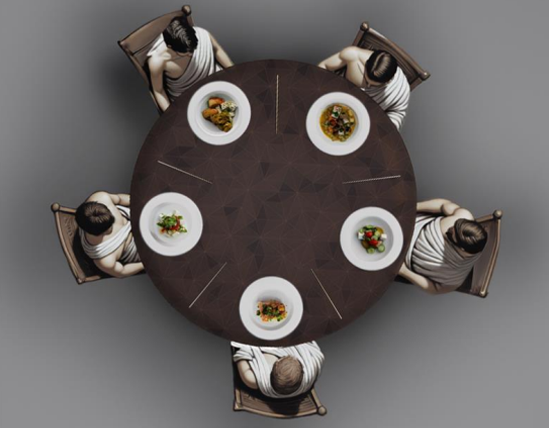
\includegraphics[width=0.7\linewidth]{Bilder/Kapitel-5/philosophen1.png}
	\caption{Das Dining Philosophers Problem}
	\label{fig:enter-label}
\end{figure}

\begin{figure}[!htbp]
	\centering
	\scalebox{0.8}{
		\petrinetz{
			\draw[colDummyLine, very thick] (-5,-5) rectangle (5,5);
			
			% neue erste Umlaufbahn: 5 Transitionen 
			
			\node[transition] (trans1)  at ({2*cos(270)}, {2*sin(270)}) {}; 
			\node[transition] (trans2)  at ({2*cos(342)}, {2*sin(342)}) {}; 
			\node[transition, label=below:$t_1$] (trans3)  at ({2*cos(54)},  {2*sin(54)})  {}; 
			\node[transition] (trans4)  at ({2*cos(126)}, {2*sin(126)}) {}; 
			\node[transition] (trans5)  at ({2*cos(198)}, {2*sin(198)}) {}; 
			
			%neue 2. Umlaufbahn 10 Stellen Philosophen und 5 Stäbchen
			
			%Stäbchen
			\node[place, tokens=1] (place6) at ({4*cos(306)}, {4*sin(306)}) {};
			\node[place, tokens=1,label=right: $s_2$] (place7) at ({4*cos(18)},  {4*sin(18)})  {};
			\node[place, tokens=1,label=above: $s_1$] (place8) at ({4*cos(90)},  {4*sin(90)})  {}; 
			\node[place, tokens=1] (place9) at ({4*cos(162)}, {4*sin(162)}) {}; 
			\node[place, tokens=1] (place10) at ({4*cos(234)}, {4*sin(234)}) {}; 
			
			%Philosphen
			
			\node[place, tokens=1] (place1) at ({3.5*cos(280)}, {3.5*sin(280)}) {}; 
			\node[place, tokens=1] (place2) at ({3.5*cos(352)}, {3.5*sin(352)}) {}; 
			\node[place, tokens=1,label=left: $d$] (place3) at ({3.5*cos(64)},  {3.5*sin(64)})  {}; 
			\node[place, tokens=1] (place4) at ({3.5*cos(136)}, {3.5*sin(136)}) {}; 
			\node[place, tokens=1] (place5) at ({3.5*cos(208)}, {3.5*sin(208)}) {}; 
			
			\node[place, tokens=0] (place11) at ({3.5*cos(260)}, {3.5*sin(260)}) {}; 
			\node[place, tokens=0] (place12) at ({3.5*cos(332)}, {3.5*sin(332)}) {};
			\node[place, tokens=0,label=right: $e$] (place13) at ({3.5*cos(44)},  {3.5*sin(44)})  {}; 
			\node[place, tokens=0] (place14) at ({3.5*cos(116)}, {3.5*sin(116)}) {}; 
			\node[place, tokens=0] (place15) at ({3.5*cos(188)}, {3.5*sin(188)}) {}; 
			
			% neue 3. Umlaufbahn: Transitionen des Gabeln wegnehmen
			\node[transition] (trans6)  at ({5*cos(270)}, {5*sin(270)}) {}; 
			\node[transition] (trans7)  at ({5*cos(342)}, {5*sin(342)}) {}; 
			\node[transition, label=above:$t_2$] (trans8)  at ({5*cos(54)},  {5*sin(54)})  {}; 
			\node[transition] (trans9)  at ({5*cos(126)}, {5*sin(126)}) {}; 
			\node[transition] (trans10)  at ({5*cos(198)}, {5*sin(198)}) {}; 
			
			% Kanten
			\draw (place1) edge[post, bend right=15](trans1);
			\draw (place2) edge[post, bend right=15](trans2);
			\draw (place3) edge[post, bend right=15](trans3);
			\draw (place4) edge[post, bend right=15](trans4);
			\draw (place5) edge[post, bend right=15](trans5);
			\draw (place6) edge[post](trans1);
			\draw (place6) edge[post](trans2);
			\draw (place7) edge[post](trans2);
			\draw (place7) edge[post](trans3);
			\draw (place8) edge[post](trans3);
			\draw (place8) edge[post](trans4);
			\draw (place9) edge[post](trans4);
			\draw (place9) edge[post](trans5);
			\draw (place10) edge[post](trans5);
			\draw (place10) edge[post](trans1);
			\draw (place11) edge[pre, bend left=15](trans1);
			\draw (place12) edge[pre, bend left=15](trans2);
			\draw (place13) edge[pre, bend left=15](trans3);
			\draw (place14) edge[pre, bend left=15](trans4);
			\draw (place15) edge[pre, bend left=15](trans5);
			%links
			\draw (place15) edge[post, bend right=15](trans10);
			\draw (place9) edge[pre](trans10);
			\draw (place10) edge[pre](trans10);
			\draw (place5) edge[pre, bend left=15](trans10);
			%oben links
			\draw (place14) edge[post, bend right=15](trans9);
			\draw (place8) edge[pre](trans9);
			\draw (place9) edge[pre](trans9);
			\draw (place4) edge[pre, bend left=15](trans9);
			
			%oben rechts
			\draw (place13) edge[post, bend right=15](trans8);
			\draw (place7) edge[pre](trans8);
			\draw (place8) edge[pre](trans8);
			\draw (place3) edge[pre, bend left=15](trans8);
			%rechts
			\draw (place12) edge[post, bend right=15](trans7);
			\draw (place6) edge[pre](trans7);
			\draw (place7) edge[pre](trans7);
			\draw (place2) edge[pre, bend left=15](trans7);
			%unten
			\draw (place11) edge[post, bend right=15](trans6);
			\draw (place10) edge[pre](trans6);
			\draw (place6) edge[pre](trans6);
			\draw (place1) edge[pre, bend left=15](trans6);
		}
	}
	\caption{Das Dining Philosophers Problem als elementares Petrinetz} \label{fig:v9_fuenf_philosophen}
\end{figure}

\pagebreak %%% für Druck

High-Level Petrinetze können nun genutzt werden, um wiederkehrende Elemente quasi „aufeinander zu falten“ (dies wird technisch tatsächlich als „folding“
\marginline{folding}
bezeichnet). Eine Stelle des High-Level Petrinetzes repräsentiert alle denkenden Philosophen, eine andere alle essenden Philosophen, und nur zwei Transitionen alle möglichen Übergänge (s.~Abb.~\ref{fig:v9_fuenf_philosophen_colored}). 


\begin{figure}[!htbp]
	\centering
	\scalebox{0.8}{
		\petrinetz{
			\draw[colDummyLine, very thick] (-1,-3) rectangle (5,3);
			
			% Places
			\node[place, tokens=0, label=left:Pd] (place1) at (0,0) {}
			[children are tokens,token distance=1.1ex]
			child {node [token,blue!30!green] {}}
			child {node [token,blue!10!green] {}}
			child {node [token,blue] {}}
			child {node [token, blue!70!green!25!white] {}}
			child {node [token, green!50!blue] {}};
			\node[place, tokens=0, label=right:S] (place2) at (2,0) {}
			[children are tokens,token distance=1.1ex]
			child {node [token,red!30!yellow] {}}
			child {node [token,red!10!yellow] {}}
			child {node [token,red!50!yellow] {}}
			child {node [token, red!70!yellow] {}}
			child {node [token, red] {}};
			
			\node[place, tokens=0, label=right:Pe] (place3) at (4,0) {};
			
			\node[transition,label=above:$t_2$] (trans1) at (2,2) {};
			\node[transition, label=below:$t_1$] (trans2) at (2,-2) {};
			
			\draw
			(place1) edge[pre, bend left=30](trans1)
			(place3) edge[post, bend right=30](trans1)
			(trans2) edge[post, bend right=30](place3)
			(trans2) edge[pre, bend left=30](place1)
			(trans1) edge[post](place2)
			%(place3) edge[post, bend left=30](trans3)
			(place2) edge[post](trans2);
			%(trans4) edge[post, bend right=30](place5)
			%(trans4) edge[post, bend left=30](place3)
			%(trans3) edge[post](place4)
			%(place4) edge[post](trans4)
			%(trans3) edge[pre, bend left=30](place5);
		}
	}
	\caption{Das Dining Philosophers Problem als Coloured Petrinetz}
	\label{fig:v9_fuenf_philosophen_colored}
\end{figure}


Natürlich müssen wir unterscheiden, welche Philosophen in einem Zustand gerade essen oder gerade denken. Und deshalb müssen wir die Marken in den Stellen unterscheiden. Wir greifen hier die Metapher der farbigen Marken auf; 
\marginline{Coloured \\ Petri Nets}
höhere Petrinetze werden oft auch „Coloured Petri Nets“ genannt \cite{jen09}.

In der Videovorlesung können sie erkennen, wie durch geeignete Kantenanschriften die Spielregeln spezifiziert werden, sodass weiterhin ein Philosoph nicht irgendwelche Stäbchen verwenden kann.

Für die Lösung besonderer Modellierungs- und Simulationsaufgaben, wie der Ermittlung von Flaschenhälsen, Optimierung von Ressourcenverteilung usw. gibt es weitere spezielle Petrinetze, die Wahrscheinlichkeiten und zeitliche Aspekte direkt berücksichtigen. Davon gibt es auch wieder viele Varianten, die teilweise im Widerspruch zu Petris Postulat der fehlenden, global verfügbaren Zeit stehen. Die wichtigsten Repräsentanten sind „Time Petri Nets“, „Timed Petri Nets“ und „Stochastic Petri Nets“. Viele Aspekte von Zeit und Wahrscheinlichkeit lassen sich aber auch durch Coloured Petri Nets modellieren.


\clearpage
\section{Vorlesung 10: Modellierung von Objektverhalten}

In den bisherigen Vorlesungen haben wir das Verhalten 
\marginline{Modellierung von Verhalten mit UML}
von Systemen und Prozessen mit Petrinetzen modelliert. In dieser und auch in der nächsten Vorlesung werden wir uns ansehen, welche Modellierungsmöglichkeiten die UML -- die ja explizit für die objektorientierte Softwareentwicklung geschaffen wurde -- für die Ver\-haltens\-model\-lierung anbietet. Dabei interessiert uns auch, welche Bezüge es zwischen diesen Diagrammen der UML und Petrinetz-Modellen gibt und an welchen Stellen man die Ihnen bekannten Prozesse, Abläufe, Aktivitäten, Aktionen etc. in den UML-Diagrammen findet.

Wir betrachten in dieser Vorlesung zunächst die Modellierung von \textbf{Objektverhalten} mithilfe der UML-Diagrammarten \textit{Zustandsdiagramm} und \textit{Sequenzdiagramm}. Vorlesung 11 wird dann mit dem UML-Aktivitätsdiagramm zurückkehren auf die Ebene der Modellierung von (Realwelt)-Prozessen.

Wir beginnen mit einem Beispiel aus dem Zookontext. Wir möchten das Verhalten eines Zoofahrzeugs modellieren, das das benötigte Futter zu den Gehegen der Tiere transportiert und beschreiben sein (mögliches) Verhalten folgendermaßen:

\vspace{2mm} %%% für Druck

\begin{addmargin}[25pt]{25pt}
	Das Fahrzeug 
	\marginline{Beispiel Zoo}
	soll seinen Standort zwischen seiner Garage und dem Futterlager wechseln können. Zudem muss es, wenn das Benzin knapp wird, an die Tankstelle fahren und wieder aufgetankt werden. Wenn sich das Zoofahrzeug am Futterlager befindet, kann es beladen werden -- abhängig davon, zu welchen Gehegen es danach fahren soll, wird es mit unterschiedlichem Futter beladen -- und fährt dann in beladenem Zustand zu seinen Zielen (z.B. Löwengehege oder Affengehege). Nach Erledigung seiner Auslieferungen kann es zurück in seine Garage fahren, zurück zum Lager, falls weiteres Futter geladen werden muss, oder auch zur Tankstelle, falls notwendig.
\end{addmargin}

\vspace{2mm} %%% für Druck

Das Verhalten des Zoofahrzeugs könnte man mit Petrinetzen abbilden, 
\marginline{Modellierung des Beispiels mit Petrinetzen}
indem man die lokalen Zustände („Tank leer“, „Tank halbvoll“, „Standort Affengehege“, „Standort Tankstelle“, „Fahrzeug mit Löwenfutter beladen“ ...) des Objekts „Fahrzeug“ durch Stellen modelliert, über die Markenverteilung auf einer Stelle dann die möglichen Objektzustände (Kombination der Wertebelegung aller Attribute des Objekts) abbildet und über die Transitionen die möglichen Änderungen der Objektzustände vorsieht. In der Videovorlesung wird ein solches Petrinetz gezeigt und erklärt.

Im objektorientierten Softwareengineering verwendet man für die Darstellung von Objektverhalten häufig das UML-Zustandsdiagramm.

\subsection*{UML-Zustandsdiagramm}

Zustandsdiagramme gehören zu den Verhaltensdiagrammen der UML. Sie basieren auf den sogenannten State Charts von David Harel \cite{har87}, wobei die Semantik allerdings etwas verändert wurde. Zustandsdiagramme werden in Softwareentwicklungsprojekten sowohl in der Anforderungsermittlung/-analyse eingesetzt -- hier meist zur Diskussion über mögliche Zustände und Verhalten von Realwelt-Objekten -- als auch im Zuge des Entwurfs des Softwareprodukts. Im letzteren Fall wird mit den Diagrammen insbesondere das gewünschte Verhalten späterer Software-Objekte spezifiziert. In beiden Fällen werden Zustandsdiagramme in der Regel in Kombination mit Klassendiagrammen verwendet, aus denen sich der Kontext ergibt, in dem das betrachtete Objekt operiert. Im Unterschied zu den Aktivitätsdiagrammen (s. Vorlesung 11), die auch Verhaltensdiagramme sind und die Aktivitäten eines Systems betrachten, konzentrieren sich Zustandsdiagramme auf die \textit{Reaktionen} von Systemelementen: in welcher Weise soll das betrachtete Objekt auf das Eintreten bestimmter Ereignisse reagieren?

Kehren wir zum Zoofahrzeug zurück und betrachten es als Objekt. Seine Zustände bedingen das mögliche Verhalten des Fahrzeugs. Schon bei solch einer noch wenig komplexen Beschreibung von Objektverhalten müssen wir für die Zustände, die das Objekt "`Zoofahrzeug"' annehmen kann, mehrere Attribute vorsehen, zum Beispiel „Füllstand des Tanks“, „Standort“, „Ladung“. Wenn wir alle möglichen Zustände (alle möglichen Kombinationen der Wertebelegungen aller Attribute) und sämtliches von diesen Zuständen abhängige mögliche Verhalten einzeln modellieren wollten, würde ein Diagramm sehr schnell unübersichtlich werden bzw. praktisch gar nicht erstellbar sein. 

Das UML-Zustandsdiagramm 
\marginline{Modellierung des Beispiels mit UML-Zustands\-diagrammen}
abstrahiert daher von den konkreten Zuständen eines Objekts und fasst mehrere Objektzustände zu einem Konstrukt (Zustand genannt!) zusammen. Also Vorsicht: ein Zustand in einem UML-Zustandsdiagramm ist in den meisten Fällen nicht gleichbedeutend mit genau einem Objektzustand, sondern umfasst eine Menge von Zuständen dieses Objekts. Zu einem Diagramm-Zustand zusammenfassen kann man alle Objektzustände, die ähnliches Verhalten zeigen, d.h. die auf gleiche Ereignisse in gleicher Weise reagieren. Zum Beispiel werden vermutlich alle Objektzustände, die mit einem halb vollen Tank des Zoofahrzeugs und alle, die mit einem dreiviertel vollen Tank zu tun haben, bezüglich ihres Verhaltens sehr ähnlich sein. 

\vspace{\baselineskip} %%% für Druck

\begin{figure}[!htbp]
	\centering
	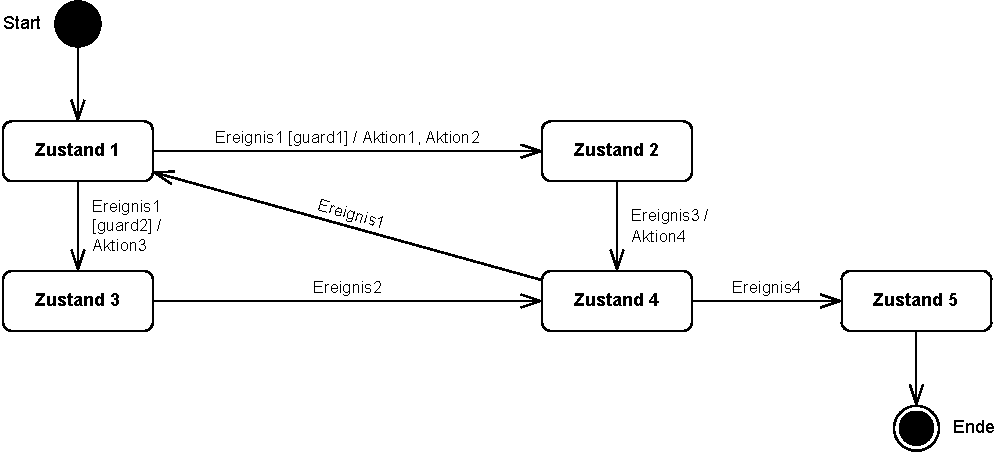
\includegraphics[scale=0.7]{Bilder/Kapitel-5/uml_zustandsdiagramm.pdf}
	\caption{Grundlegende Elemente eines UML-Zustandsdiagramms}
	\label{fig:uml_zustandsdiagramm}
\end{figure}

\vspace{\baselineskip} %%% für Druck

Abbildung~\ref{fig:uml_zustandsdiagramm} zeigt die wichtigsten Elemente eines UML-Zustandsdiagramms. 
\marginline{Zustände}
Die \textit{Zustände} werden mit abgerundeten Rechtecken modelliert. Das modellierte Objekt befindet sich immer in genau einem Zustand -- in Petrinetz-Terminologie gedacht: es gibt genau eine Marke und diese befindet sich in dem Zustand, in dem das Objekt gerade ist. Die gerichteten Pfeile modellieren die Übergänge zwischen den Zuständen, sie heißen \textit{Transitionen}.
\marginline{Transitionen}
Der Übergang von einem Zustand in einen anderen wird ausgelöst durch ein \textit{Ereignis}. Das auslösende Ereignis wird als Beschriftung an die Transition notiert. Die UML unterscheidet verschiedene Formen von Ereignissen. Die wichtigsten sind das \textit{Call Event} (Anfrage) -- dieses findet man häufig in Form von Operationsaufrufen in Zustandsdiagrammen, die im Rahmen des Entwurfsprozesses erstellt werden -- das \textit{Signal Event} (asynchrones Signal), das \textit{Time Event} (Abhängigkeit von Zeit) und das \textit{Change Event} (Bedingung).

\vspace{0.9mm} %%% für Druck

Wenn ein Ereignis eintritt, 
\marginline{Ereignis} 
wechselt das Objekt in den durch die entsprechende Transition definierten Folgezustand. „Auf diesem Weg“ können zudem Aktivitäten stattfinden, und zwar sowohl Aktivitäten, 
\marginline{Aktivitäten}
die durch das Objekt selber durchgeführt werden, als auch Aktivitäten anderer Objekte im umgebenden System. In letzterem Fall kann ein Zustandsdiagramm ohne Kenntnis des Kontextes (z.B. durch vorliegende andere UML-Diagramme) für die Leser aber schnell unverständlich werden. Aktivitäten werden im Zustandsdiagramm ebenfalls an den Transitionen notiert, vom Ereignis jeweils getrennt durch einen Schrägstrich („/“). 

\vspace{0.9mm} %%% für Druck

Dasselbe Ereignis kann durchaus mehrfach im Zustandsdiagramm vorkommen. Je nachdem, von welchem Zustand die zugehörige Transition ausgeht, wird es aber unterschiedliches Verhalten des Objekts auslösen. Zum Beispiel könnte das Zeitereignis „Mittagszeit“ dafür sorgen, dass das Zoofahrzeug zum Löwengehege fährt, sofern es Löwenfutter geladen hat. Hat es dagegen Affenfutter geladen, sollte dasselbe Ereignis dazu führen, dass es zum Affengehege fährt. Hat das Fahrzeug Affenfutter geladen und gleichzeitig kaum noch Benzin im Tank, wird es wieder ein anderes Verhalten zeigen und vor der Fahrt zum Affengehege noch die Tankstelle aufsuchen.

\vspace{0.9mm} %%% für Druck

Man kann Zustandsdiagramme mit einem Startzustand 
\marginline{Start- und Endzustände}
und einem oder mehreren Endzuständen ausstatten. Ein schwarz ausgefüllter Kreis kennzeichnet den Startzustand, ein weißer Kreis mit schwarzem Punkt -- der leider so aussieht wie bei Petrinetzen ein lokaler Startzustand -- einen Endzustand.

\vspace{0.9mm} %%% für Druck

In Zustandsdiagrammen ist Nichtdeterminismus ein Fehlerfall, 
\marginline{Nicht\-determinismus}
eine Konstruktion wie in Abbildung~\ref{fig:zustandsdiagramme} oben darf daher nicht vorkommen. Hier ist nicht eindeutig festgelegt, in welchen der drei Zustände das Objekt wechseln soll, wenn das Ereignis „Mittagszeit“ eintritt. Die gängigste Variante eine solche Situation deterministisch zu modellieren, ist die Verwendung von \textit{Guards}.
\marginline{Guard}
Abbildung~\ref{fig:zustandsdiagramme} unten zeigt diese Lösung. Der Guard, eine Bedingung, die sich zum Beispiel auf einen Attributwert des Objekts beziehen kann, wird in eckigen Klammern hinter das Ereignis geschrieben. Die verschiedenen Guards an den Transitionen müssen so formuliert werden, dass immer nur höchstens einer der Guards desselben Ereignisses zutrifft. Es sollte auch nicht der Fall eintreten, dass keiner der Guards zutrifft; das wäre zwar nach Diagramm-Regeln nicht verboten, macht semantisch aber keinen Sinn. 


\begin{figure}[t]
	\vspace{5mm} %%% für Druck
	\centering
	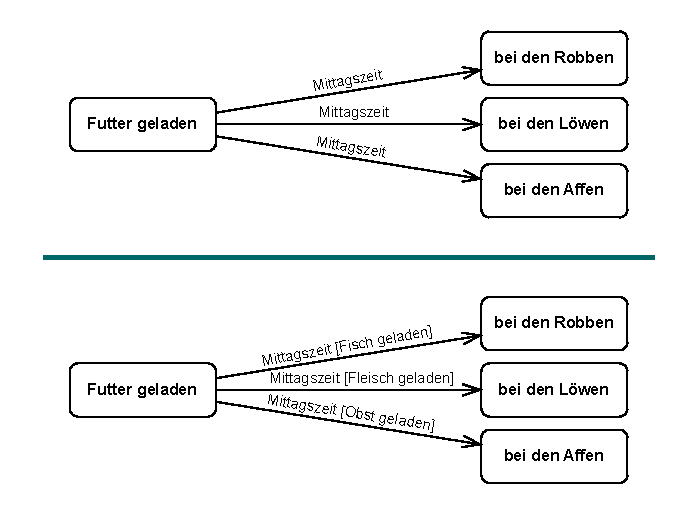
\includegraphics[scale=1.0]{Bilder/Kapitel-5/zustandsdiagramme.pdf}
	\caption[Ein fehlerhaftes nichtdeterministisches und ein korrektes deterministisches Zustandsdiagramm]{Ein fehlerhaftes nichtdeterministisches (oben) und ein korrektes deter\-ministisches (unten) Zustandsdiagramm}
	\label{fig:zustandsdiagramme}
	\vspace{\baselineskip} %%% für Druck
\end{figure}


\vspace{0.9mm} %%% für Druck

Neben den vorgestellten Grundelementen bietet die UML für Zustandsdiagramme einige weitere Elemente an, mit denen man Verhalten detaillierter spezifizieren kann. Darunter sind auch Möglichkeiten Verzweigungen und Schleifen zu modellieren, die man häufig benötigt, wenn Zustandsdiagramme (für Software-Objekte) schon sehr implementierungsnah sein sollen. Bei Diagrammen mit sehr vielen modellierten Zuständen lohnt sich zudem der Einsatz des Elements „zusammengesetzter Zustand“ (wird in der Videovorlesung an einem Beispiel gezeigt), mit dem man Hierarchien von Zuständen darstellen kann.

\subsection*{UML-Sequenzdiagramm}

Auch mit den UML-Sequenzdiagrammen modelliert man Verhalten, aber nicht nur das Verhalten eines einzelnen Objekts, sondern vor allem die Kommunikation (Austausch von Nachrichten) zwischen Objekten. 

Sequenzdiagramme haben ihren Ursprung in den Message Sequence Charts aus dem Telekommunikationsbereich, auch wenn der Blick dort nicht auf Objekte, sondern auf größere Einheiten gerichtet war. Im Softwareengineering kann man Sequenzdiagramme während der Anforderungsermittlung einsetzen, um Nachrichtenflüsse zwischen Personen oder Systemkomponenten in Geschäftsprozessen, die das spätere Softwareprodukt unterstützen soll, deutlich zu machen. Wesentlich häufiger werden Sequenzdiagramme aber beim Entwurf eingesetzt und sind schon sehr implementierungsnah. Auch die Reaktion des Softwareystems auf die Bedienung der GUI durch den Nutzer (was genau passiert, wenn der Nutzer diesen Button klickt, dieses Menü öffnet etc.) ist ein typischer Einsatzzweck eines Sequenzdiagramms.

Kehren wir kurz nochmal zu den Petrinetzen zurück und überlegen, wie wir Objektkommunikation mit Petrinetzen modellieren würden.

\pagebreak %%% für Druck

\begin{figure}[!htbp]
	\vspace{5mm} %%% für Druck
	\centering
	\begin{tabular}{ll}
		%--------------------------------------
		% \hline
		% 1. Reihe
		\textbf{Objekte} & 
		\parbox{0.75\textwidth}{
			\scalebox{0.6}{
				\petrinetz{
					\draw[colDummyLine, very thick] (-0.5, -1) rectangle (16.5, 1);
					
					% Places
					\node[place, tokens=1, label=above:$s_2$] (s2) at ( 6,  2) {}; 
					\node[place, tokens=0, label=below:$s_4$] (s4) at ( 6, -2) {}; 
					\node[place, tokens=0, label=right:$s_3$] (s3) at (10,  0) {}; 
					
					% Transitions
					\node[transition, label=left: $t_2$] (t2) at (4,  0) {}; 
					\node[transition, label=above:$t_3$] (t3) at (8,  2) {}; 
					\node[transition, label=below:$t_5$] (t5) at (8,  0) {};
					\node[transition, label=below:$t_4$] (t4) at (8, -2) {};
					
					%Edges
					\draw 
					(t2) edge[post, bend left=30] (s2) 
					(s2) edge[post] (t3) 
					(t3) edge[post, bend left=30] (s3) 
					(s3) edge[post] (t5) 
					(s3) edge[post, bend left=30] (t4) 
					(t4) edge[post] (s4) 
					(t5) edge[post, bend left=30] (s2) 
					(s4) edge[post, bend left=30] (t2)
					;
					
					%					\draw (s2) edge[post] (t3);
					%					\draw (t3) edge[post] (s3);
					%					\draw (s3) edge[post] (t4);
					%					\draw (t4) edge[post] (s4);
					%					\draw (s4) edge[post] (t2);
					%					\draw (t2) edge[post] (s2);
					%					\draw (s3) edge[post] (t5);
					%					\draw (t5) edge[post] (s2);
				}
			}
		}
		\\
		%--------------------------------------
		%--------------------------------------
		% \hline
		&  \\ % eine Leerzeile für den Abstand
		&  \\ % eine Leerzeile für den Abstand
		&  \\ % eine Leerzeile für den Abstand
		%--------------------------------------
		% \hline
		% 2. Reihe
		\textbf{Ablauf} & 
		\parbox{0.75\textwidth}{
			\scalebox{0.6}{
				\petrinetz{
					\draw[colDummyLine](-0.5, 0) -- (16.5, 0);
					
					% Places
					\node[place, tokens=1, label=above:$s_2$] (place2_1) at ( 0, 0) {};
					\node[place, tokens=0, label=above:$s_3$] (place3_1) at ( 4, 0) {};
					\node[place, tokens=0, label=above:$s_2$] (place2_2) at ( 8, 0) {};
					\node[place, tokens=0, label=above:$s_3$] (place3_2) at (12, 0) {};
					\node[place, tokens=0, label=above:$s_4$] (place4)   at (16, 0) {};
					
					% Transitions
					\node[transition, label=center:$t_3$] (trans3_1) at ( 2, 0) {};
					\node[transition, label=center:$t_5$] (trans5)   at ( 6, 0) {};
					\node[transition, label=center:$t_3$] (trans3_2) at (10, 0) {};
					\node[transition, label=center:$t_4$] (trans4)   at (14, 0) {};
					
					% Edges
					\draw (place2_1) edge[post] (trans3_1);
					\draw (trans3_1) edge[post] (place3_1);
					\draw (place3_1) edge[post] (trans5);
					\draw (trans5)   edge[post] (place2_2);
					\draw (place2_2) edge[post] (trans3_2);
					\draw (trans3_2) edge[post] (place3_2);
					\draw (place3_2) edge[post] (trans4);
					\draw (trans4)   edge[post] (place4);
				}
			}
		}
		\\
		%--------------------------------------
		%--------------------------------------
		% \hline
		&  \\ % eine Leerzeile für den Abstand
		&  \\ % eine Leerzeile für den Abstand
		&  \\ % eine Leerzeile für den Abstand
		%--------------------------------------
		% \hline
		% 3. Reihe
		\textbf{Kommunikation} & 
		\parbox{0.75\textwidth}{
			\scalebox{0.6}{
				\petrinetz{
					\draw[colDummyLine, very thick] (-0.5, -5) rectangle (16.5, 1);
					
					% Places
					\node[place, tokens=1] (s1) at (0,  0) {};
					\node[place, tokens=0] (s2) at (4,  0) {};
					\node[place, tokens=0] (s3) at (8,  0) {};
					\node[place, tokens=0] (s4) at (12, 0) {};
					\node[place, tokens=0] (s5) at (16, 0) {};
					
					\node[place, tokens=0] (s6) at (2,  -2) {};
					\node[place, tokens=0] (s7) at (10, -2) {};
					\node[place, tokens=0] (s8) at (12, -2) {};
					
					\node[place, tokens=1] (s9)  at (0,  -4) {};
					\node[place, tokens=0] (s10) at (4,  -4) {};
					\node[place, tokens=0] (s11) at (8,  -4) {};
					\node[place, tokens=0] (s12) at (12, -4) {};
					\node[place, tokens=0] (s13) at (16, -4) {};
					
					% Transitions
					\node[transition] (t1) at (2,  0) {};
					\node[transition] (t2) at (6,  0) {};
					\node[transition] (t3) at (10, 0) {};
					\node[transition] (t4) at (14, 0) {};
					
					\node[transition] (t5) at (2,  -4) {};
					\node[transition] (t6) at (6,  -4) {};
					\node[transition] (t7) at (10, -4) {};
					\node[transition] (t8) at (14, -4) {};
					
					% Edges
					% obere Reihe
					\draw (s1) edge[post] (t1);
					\draw (t1) edge[post] (s2);
					\draw (s2) edge[post] (t2);
					\draw (t2) edge[post] (s3);
					\draw (s3) edge[post] (t3);
					\draw (t3) edge[post] (s4);
					\draw (s4) edge[post] (t4);
					\draw (t4) edge[post] (s5);
					
					% untere Reihe
					\draw (s9)  edge[post] (t5);
					\draw (t5)  edge[post] (s10);
					\draw (s10) edge[post] (t6);
					\draw (t6)  edge[post] (s11);
					\draw (s11) edge[post] (t7);
					\draw (t7)  edge[post] (s12);
					\draw (s12) edge[post] (t8);
					\draw (t8)  edge[post] (s13);
					
					% dazwischen
					\draw (t1) edge[post] (s6);
					\draw (s6) edge[post] (t5);
					\draw (t3) edge[post] (s7);
					\draw (s7) edge[post] (t7);
					\draw (t7) edge[post] (s8);
					\draw (s8) edge[post] (t4);
				}
			}
		}
		\\
		%\hline
	\end{tabular}
	\vspace{\baselineskip} %%% für Druck
	\caption{Kommunikation zwischen Objekten in Petrinetz-Modellierung}
	\label{fig:kommunikation_zw_objekten}
\end{figure}


Abbildung~\ref{fig:kommunikation_zw_objekten} zeigt oben ein Petrinetz, mit dem wir das mögliche Verhalten von uns interessierenden Objekten modelliert haben. In der Mitte ist ein möglicher Ablauf für ein konkretes Objekt dargestellt. Dieser Ablauf ist rein sequentiell, weil das Objektverhalten keinerlei Nebenläufigkeit aufweist. Unten in der Abbildung sehen Sie Abläufe von zwei verschiedenen Objekten, wobei wir in der Abbildung nicht dargestellt haben, welche Transitionen genau geschaltet wurden (die zwei horizontalen Ketten aus unbeschrifteten Stellen und Transitionen). Die Kommunikation der beiden Objekte modellieren wir, indem wir ihre Abläufe an den Positionen, an denen Kommunikation stattfindet, über Stellen miteinander verbinden. Hier schicken sich die beiden Objekte Nachrichten (z.B. Operationsaufrufe). Bei der links dargestellten Kommunikation handelt es sich um eine \textit{asynchrone}, rechts um eine \textit{synchrone} Nachricht. 
\marginline{synchrone und asynchrone Kommunikation}
Bei asynchroner Kommunikation kann der Sender mit seiner Arbeit fortfahren, unabhängig davon, wann und ob der Empfänger antwortet. Bei synchroner Kommunikation geht das nicht, der Sender wartet so lange, bis er eine Antwort erhält. Sie sehen daher rechts in der Abbildung, dass die nächste Transition des oberen Ablaufs erst schalten kann, nachdem die Transition des unteren Ablaufs geschaltet hat. Wo keine Kommunikation stattfindet, können die Objekte unabhängig voneinander, also nebenläufig agieren.

\pagebreak %%% für Druck

Die Modellierung von Objektkommunikation durch UML-Sequenzdiagramme funktioniert sehr ähnlich. Abbildung~\ref{fig:uml_sequenzdiagramm} zeigt die grundlegenden Elemente eines 
\linebreak %%% für Druck
Sequenzdiagramms. 


\begin{figure}[!htbp]
	\centering
	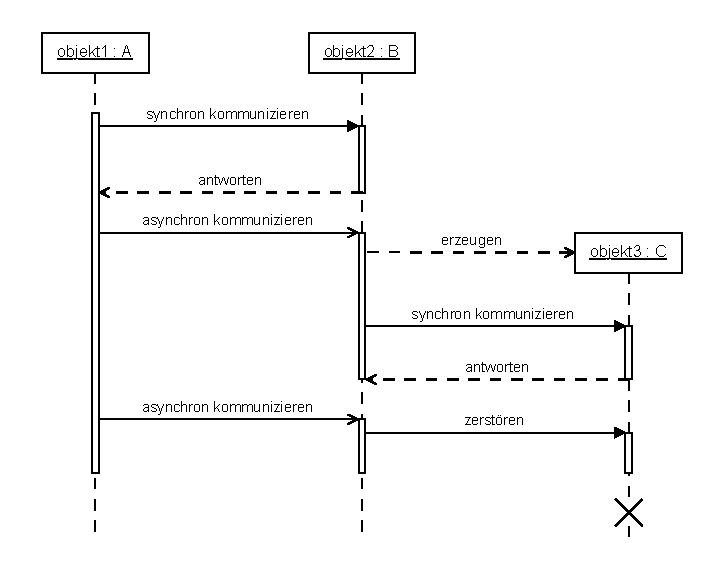
\includegraphics[scale=1.0]{Bilder/Kapitel-5/uml_sequenzdiagramm.pdf}
	\caption{Grundlegende Elemente eines UML-Sequenzdiagramms}
	\label{fig:uml_sequenzdiagramm}
\end{figure}


Statt von links nach rechts wie in unserer Petrinetz-Abbildung werden die Abläufe der Objekte von oben nach unten gezeichnet, symbolisiert durch die gestrichelten Linien, die man \textit{Lebenslinien} 
\marginline{Lebenslinie}
nennt. Die verschiedenen Objekte, die miteinander kommunizieren, sind dementsprechend horizontal nebeneinander angeordnet und werden wie im Klassendiagramm jeweils durch ein Rechteck dargestellt. Die Darstellung als anonymes Objekt einer Klasse geht auch. Zudem können auch menschliche Teilnehmer an der Interaktion modelliert werden (wie in anderen UML-Diagrammen als Strichmännchen). 

Sequenzdiagramme können durchaus die Kommunikation zwischen mehreren Objekten derselben Klasse modellieren. In der Regel interessiert aber die Kommunikation zwischen Objekten verschiedener Klassen. Man sieht sich im Sequenzdiagramm somit die Details genau der Beziehungen an, die man in Klassendiagrammen mit Assoziationen und Multiplizitäten modelliert hat.

Während mit der Lebenslinie im Sequenzdiagramm die komplette Lebenszeit eines Objekts symbolisiert wird, kennzeichnen die weißen Balken auf der Lebenslinie -- sie heißen \textit{Ausführungsbalken}
\marginline{Ausführungs\-balken}
-- die aktive Phase des Objekts. Synchrone und asynchrone Nachrichten werden durch unterschiedliche Pfeilspitzen dargestellt, die Antwort auf eine synchrone Nachricht durch einen gestrichelten Pfeil (s.~Abb.~\ref{fig:uml_sequenzdiagramm}). 

\pagebreak %%% für Druck

Zwei besondere Kommunikationsarten sind die Anforderung zur Erzeugung 
\marginline{Erzeugung und Zerstörung}
und zur Zerstörung eines Objekts. Die Erzeugungsanforderung, die dieselbe Pfeilart wie die Antwortnachricht hat, erkennt man daran, dass die Pfeilspitze nicht an einer Lebenslinie endet, sondern direkt an dem Objekt, das erzeugt wird. Die Zerstörungsanforderung gleicht syntaktisch einer synchronen Nachricht. Man erkennt sie -- neben der Tatsache, dass sie zumeist mit „zerstören“ beschriftet ist -- an dem großen {\Large$\times$} (ein sogenanntes Stopp-Symbol, das es in mehreren UML-Diagrammarten gibt) auf der Lebenslinie kurz unterhalb der eingehenden Nachricht.

Auch mit Sequenzdiagrammen kann man noch sehr viel detaillierter modellieren, zum Beispiel durch übereinanderliegende Ausführungsbalken parallele Tätigkeiten des Objekts vorsehen oder über sogenannte Zustandsinvarianten die Teilnahme eines Objekts an der Kommunikation von seinem aktuellen Zustand abhängig machen. Für viele Einsatzzwecke im Softwareengineering reichen die grundlegenden Elemente des Sequenzdiagramms aber aus.

\clearpage
\section{Vorlesung 11: Andere Prozessbeschreibungssprachen}

In dieser Vorlesung betrachten wir UML-Aktivitätsdiagramme und Bezüge dieser Modellierungssprache zu Petrinetzen.

Aktivitätsdiagramme 
\marginline{Aktivitäts\-diagramme}
sind eigentlich geklaute Petrinetze mit einer anderen Syntax und ergänzenden Notationen, aber derselben Semantik. Wie Petrinetze kann man Aktivitätsdiagramme sowohl zur Modellierung von Prozessen als auch zur Modellierung von Abläufen einsetzen, allgemeinere Systeme sind dagegen nicht im Fokus von Aktivitätsdiagrammen. Man kann sie in unterschiedlichen Abstraktionsgraden und für unterschiedliche Zwecke in allen Kernprozessen des Softwareengineering verwenden. Sie sind extrem mächtig, da sie sehr viele unterschiedliche Notationselemente zur Verfügung stellen.

Während der Anforderungsermittlung 
\marginline{Einsatzbereiche}
in einem Softwareentwicklungsprojekt werden Aktivitätsdiagramme häufig zur Darstellung von Geschäftsprozessen der Real\-welt verwendet. Ein zweiter Einsatzbereich ist die differenziertere Modellierung von Abläufen der Anwendungsfälle aus einem UML-Anwendungsfalldiagramm (dieses lernen Sie in Lektion~4 kennen). Beides erfolgt stark Nutzersicht-zentriert, dafür wird in der Regel nur ein Bruchteil der zur Verfügung stehenden Notationselemente benötigt. Aber auch für den implementierungsnahen Einsatz bieten Aktivitäts\-diagramme viele Möglichkeiten. So lassen sich sowohl interne Systemprozesse als auch Algorithmen mit ihnen modellieren. Dafür kommen dann auch etwas komplexere Notationsmöglichkeiten des Diagrammtyps wie Schleifen, Zustandsvariablen oder Ausnahmebehandlungen zum Tragen.


\begin{figure}
	\centering
	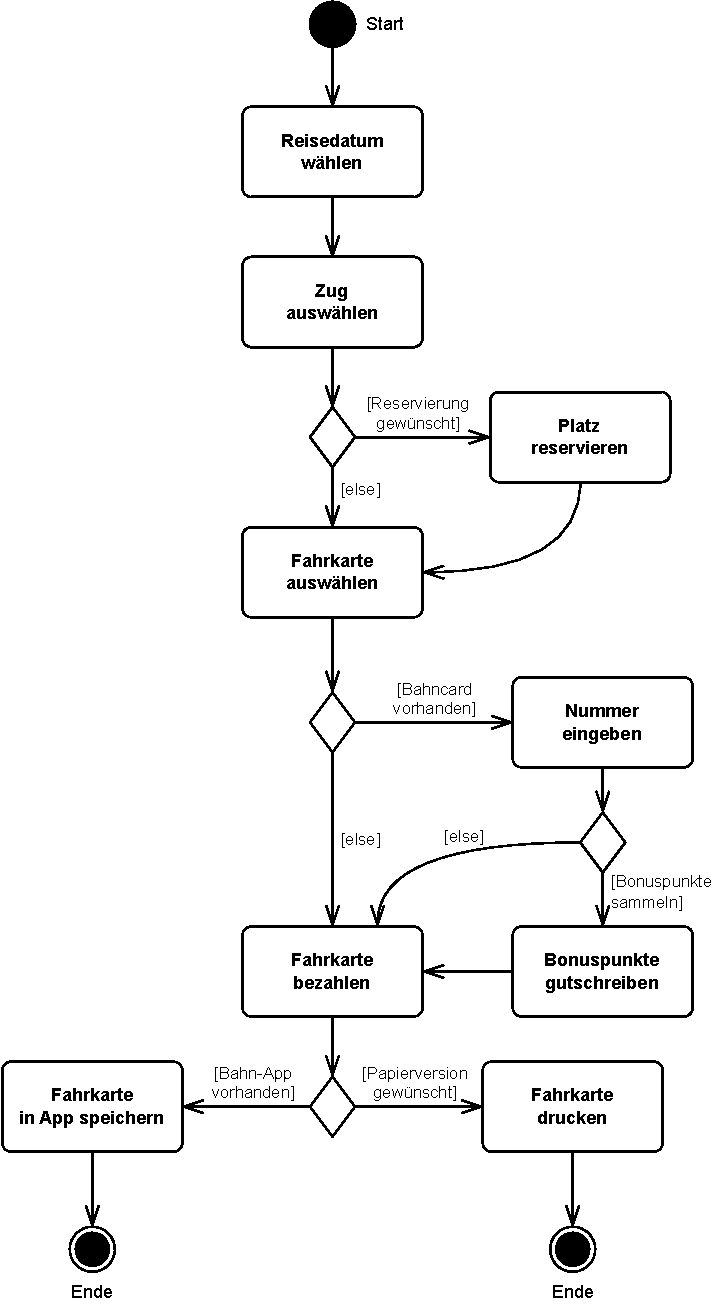
\includegraphics[scale=0.7]{Bilder/Kapitel-5/aktivitaetsdiagramm_fahrkarte_kaufen.pdf}
	\caption{Aktivitätsdiagramm für die Aktivität Fahrkartenkauf}
	\label{fig:aktivitaetsdiagramm_fahrkarte_kaufen}
\end{figure}

Abbildung~\ref{fig:aktivitaetsdiagramm_fahrkarte_kaufen} zeigt ein Aktivitätsdiagramm für eine \textit{Aktivität} Fahrkartenkauf. Vorsicht: das Aktivitätsdiagramm unterscheidet nicht sauber zwischen Prozessebene und Ablaufebene! Die Benennungen „Aktivität“ und „Aktion“ werden auf derselben Ebene verwendet, und sie bedeuten etwas anderes als bei uns. Auch wird nicht unterschieden, ob es um ein Prozessmodell oder um den modellierten Prozess geht. 

Als Aktivität wird der Prozess als Gesamtes bezeichnet, 
\marginline{Syntax und Semantik}
also hier die Aktivität "`Fahrkartenkauf"'. Die einzelnen \textit{Schritte} in dieser Aktivität sind die \textit{Aktionen}, wie „Reisedatum auswählen“ oder „Fahrkarte bezahlen“. Diese werden mit abgerundeten Rechtecken dargestellt. Die Pfeile repräsentieren den Kontrollfluss, die Ausführungsreihenfolge zwischen den Aktionen. Wie im Zustandsdiagramm ist der schwarz ausgemalte Kreis der Startknoten, der spezifiziert, bei welcher Aktion die Aktivität Fahrkartenkauf beginnt.

Die Rauten sind sogenannte \textit{Entscheidungsknoten}. Ein Entscheidungsknoten hat genau einen eingehenden Kontrollfluss und beliebig viele ausgehende, von denen bei einer konkreten Ausführung der Aktivität aber nur genau einer fortgeführt wird. Die ausgehenden Pfeile des Entscheidungsknotens sind mit Bedingungen (Guards) versehen, die wie bei höheren Petrinetzen und bei Zustandsdiagrammen in eckigen Klammern notiert werden. Auch hier die Parallele zu den Zustandsdiagrammen: die Guards eines Entscheidungsknotens müssen sich gegenseitig ausschließen und sollten alle Auswahlmöglichkeiten abdecken, so dass der weitere Kontrollfluss eindeutig festgelegt ist. Ein oder mehrere Endknoten (schwarzer Kreis mit weißer Umrandung) spezifizieren, nach welchen Aktionen eine Aktivität enden kann.

Analog zum Element \textit{Entscheidungsknoten} bietet das Aktivitätsdiagramm auch einen \textit{Verbindungsknoten} an, wenn Kontrollflüsse wieder zusammenlaufen. Dieser wird ebenfalls über eine Raute dargestellt. Er unterscheidet sich vom Entscheidungsknoten dadurch, dass beliebig viele Kontrollflüsse hereinführen, aber nur genau einer herausführt. Häufig lässt man Verbindungsknoten im Diagramm weg und führt die Kontrollflüsse direkt in der Aktion wieder zusammen -- so auch hier in der Abbildung. Die UML erlaubt es, in ähnlicher Weise auch auf die Entscheidungsknoten zu verzichten, aber das macht ein Aktivitätsdiagramm meistens unübersichtlicher. Zumindest bei Aktivitätsdiagrammen im Rahmen der Anforderungsermittlung sollte man Entscheidungsknoten daher nicht weglassen.


\begin{figure}[h!]
	\centering
	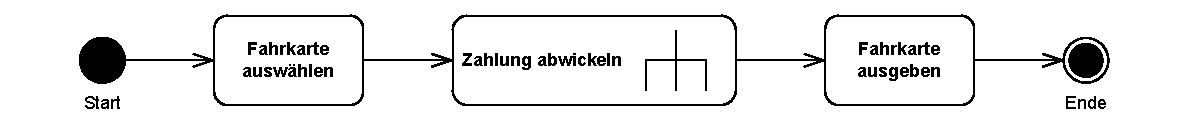
\includegraphics[scale=0.7]{Bilder/Kapitel-5/aktivitaetsaufruf_zahlung.pdf}
	\caption{Aktivitätsaufruf "`Zahlung abwickeln"'}
	\label{fig:aktivitaetsaufruf_zahlung}
\end{figure}

\begin{figure}[h!]
	\centering
	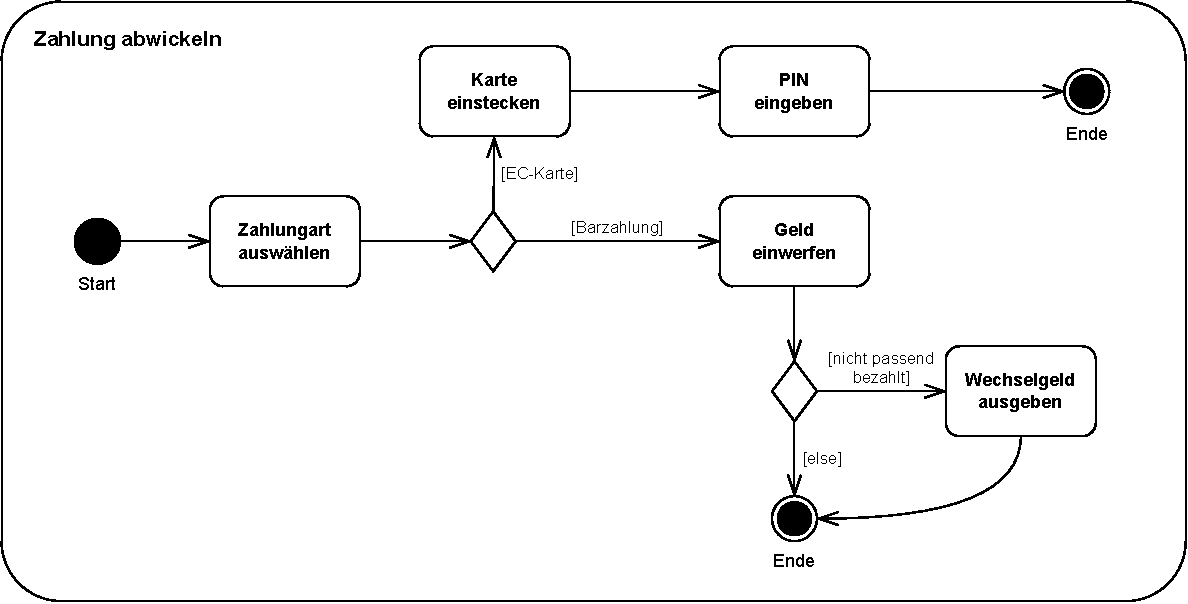
\includegraphics[scale=0.7]{Bilder/Kapitel-5/aktivitaetsdiagramm_zahlung_abwickeln.pdf}
	\caption{Aktivitätsdiagramm "`Zahlung abwickeln"'}
	\label{fig:aktivitaetsdiagramm_zahlung_abwickeln}
\end{figure}

Wenn Aktivitäten sehr kleinschrittig (viele einzelne Aktionen) beschrieben werden sollen, können Aktivitätsdiagramme schnell unübersichtlich werden. Oft bietet es sich an, ein Aktivitätsdiagramm auf einem hohen Abstraktionsniveau als Übersicht zu haben und dessen einzelne Aktionen in jeweils eigenen Diagrammen verfeinert zu modellieren. Abbildung~\ref{fig:aktivitaetsaufruf_zahlung} zeigt ein sehr übersichtliches Diagramm für eine Aktivität „Fahrkarte kaufen“ an einem Automaten. Bei der Aktion „Zahlung abwickeln“ in diesem Diagramm ist durch das Gabel-Symbol rechts im Kästchen gekennzeichnet, dass hier ein Aktivitätsaufruf erfolgt, und zwar der Aufruf der Aktivität „Zahlung abwickeln“, die in einem eigenen Aktivitätsdiagramm modelliert ist. Dieses ist in Abbildung~\ref{fig:aktivitaetsdiagramm_zahlung_abwickeln} dargestellt.
 
\pagebreak %%% für Druck

Im Rahmen der Domänenmodellierung werden Aktivitätsdiagramme vor allem zur Modellierung von Geschäftsprozessen der Domäne eingesetzt. Häufig geht es dabei auch darum herauszufinden, welche Akteure in welcher Art und Weise am Geschäftsprozess beteiligt sind, also wer welche Tätigkeiten im Rahmen des Geschäfts\-prozesses ausführt. Das UML-Aktivitätsdiagramm bietet das Element \textit{Aktivitäts\-bereich} an, um die Verantwortung für Aktionen bestimmten Akteuren zuzuordnen. Dies ist ein ähnliches Konzept wie Pools und Lanes in BPMN. Abbildung~\ref{fig:aktivitaetsdiagramm_futterannahme} zeigt ein Diagramm mit drei Aktivitätsbereichen für die Akteure „Tierpfleger“, „Lager\-verwalter“ und „Zooverwaltung“ für eine Aktivität „Futterannahme“. Durch die Platzierung in den Aktivitätsbereichen ist deutlich, wer welche Aktionen ausführt.
  

\begin{figure}[h!]
	\centering
	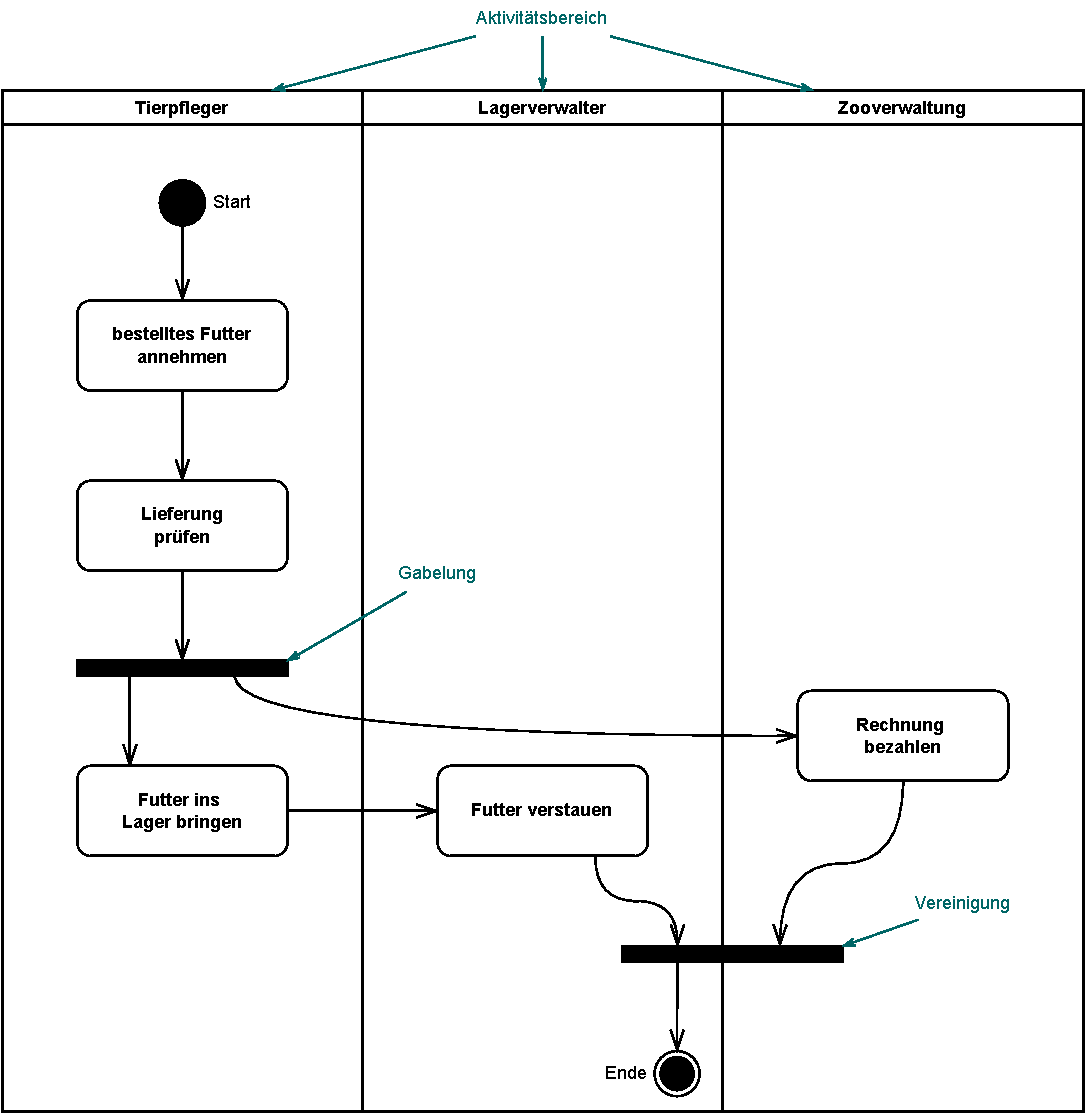
\includegraphics[scale=0.7]{Bilder/Kapitel-5/aktivitaetsdiagramm_futterannahme.pdf}
	\caption{Aktivitätsdiagramm Futterannahme}
	\label{fig:aktivitaetsdiagramm_futterannahme}
\end{figure}

Abbildung~\ref{fig:aktivitaetsdiagramm_futterannahme} zeigt außer den Aktivitätsbereichen auch die Elemente für die Model\-lie\-rung
sogenannter \textit{Gabelungen} (oberer schwarzer Balken). Diese sind unabhängig von den Aktivitätsbereichen, hätten also auch in den vorherigen Diagrammen verwendet werden können. Die Gabelung teilt einen Kontrollfluss in mehrere Kontrollflüsse auf, die nebenläufig laufen. Das Pendant, um die Nebenläufigkeit wieder zu beenden, ist die sogenannte \textit{Vereinigung}, die Sie rechts unten im Diagramm sehen. Die Vereinigung fasst mehrere Kontrollflüsse zu einem Kontrollfluss zusammen. Hier in der Abbildung modelliert sie, dass sowohl die Aktion „Futter verstauen“ vom Akteur „Lagerverwalter“ als auch die Aktion „Rechnung bezahlen“ vom Akteur „Zooverwaltung“ abgeschlossen sein müssen, bevor die Aktivität „Futterannahme“ beendet ist. Dieses Beispiel erinnert eher an einen halbgeordneten Petrinetz-Ablauf.

Sicherlich sind Ihnen die Ähnlichkeiten zwischen Aktivitätsdiagrammen und Petri\-netzen bereits aufgefallen. Die folgende Tabelle zeigt nochmal eine Gegenüber\-stellung verschiedener Elemente in der Syntax der beiden Prozess\-beschreibungs\-sprachen. In der Vorlesung werden zusätzlich die Ähnlichkeiten der Petrinetze zu den aus Vor\-lesung~1 bekannten Geschäftsprozess-Modellierungssprachen EPK und BPMN aufgezeigt.


\begingroup
	\setlength{\tabcolsep}{10pt} % Default value: 6pt
	\renewcommand{\arraystretch}{1.5} % Default value: 1
	
	% Hilfsvariablen
	\newcommand{\sttpHilfA}{0.25\textwidth} % Breite der linken Spalte	(Beschreibung)
	\newcommand{\sttpHilfB}{0.25\textwidth} % Breite der der mittleren und der rechten Spalte(Abbildungen)
	\newcommand{\sttpFaktor}{0.8} % Skalierungsfaktor für die Grafiken
	\newcommand{\sttpAbstandRand}{5mm}
	
	% Die einzelnen Grafiken wurden mit einer Rahmenbreite von "0" in DrawIO exportiert.
	
	%\begin{figure}[!htbp]
	%	\centering
	\begin{longtable}{p{\sttpHilfA}|c|c}

		% \hline %-----------------------------

			\parbox{\sttpHilfA}{\centering
				\textbf{Element}} 
		&
			\textbf{Aktivitätsdiagramm} 
		&
			\textbf{Petrinetze} 
		\\
			
		\hline %-----------------------------
		\hline %-----------------------------
		\endhead
		
			\parbox{\sttpHilfA}{\centering
				Aktivität}
		&
			\parbox{\sttpHilfB}{\centering
				\vspace{\sttpAbstandRand}
				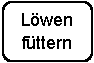
\includegraphics[scale=\sttpFaktor]{Bilder/Kapitel-5/gegenueberstellung_1a.pdf}
				\vspace{\sttpAbstandRand}
			} 
		&
			\parbox{\sttpHilfB}{\centering
				\vspace{\sttpAbstandRand}
				
\includegraphics[scale=\sttpFaktor]{Bilder/Kapitel-5/gegenueberstellung_1b.pdf}
				\vspace{\sttpAbstandRand}
			} 
		\\
		
		\hline %-----------------------------
		
			\parbox{\sttpHilfA}{\centering
				Vor- und \\ Nachbedingung} 
		& 
			\parbox{\sttpHilfB}{\centering
				\vspace{\sttpAbstandRand}
				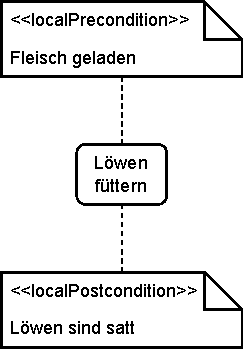
\includegraphics[scale=\sttpFaktor]{Bilder/Kapitel-5/gegenueberstellung_2a.pdf}
				\vspace{\sttpAbstandRand}
			} 
		&
			\parbox{\sttpHilfB}{\centering
				\vspace{\sttpAbstandRand}
				
\includegraphics[scale=\sttpFaktor]{Bilder/Kapitel-5/gegenueberstellung_2b.pdf}
				\vspace{\sttpAbstandRand}
			} 
		\\
	
		\hline %-----------------------------
	
			\parbox{\sttpHilfA}{\centering
				Kontrollfluss}
		&  
			\parbox{\sttpHilfB}{\centering
				\vspace{\sttpAbstandRand}
				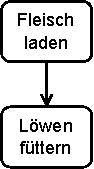
\includegraphics[scale=\sttpFaktor]{Bilder/Kapitel-5/gegenueberstellung_3a.pdf}
				\vspace{\sttpAbstandRand}
			}
		& 
			\parbox{\sttpHilfB}{\centering
				\vspace{\sttpAbstandRand}
				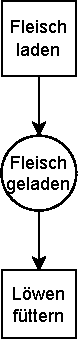
\includegraphics[scale=\sttpFaktor]{Bilder/Kapitel-5/gegenueberstellung_3b.pdf}
				\vspace{\sttpAbstandRand}
			}
		\\
		
		\hline %-----------------------------
		
			\parbox{\sttpHilfA}{\centering
				Aktivitätsbereich \\ / \\ Komponente} 
		& 
			\parbox{\sttpHilfB}{\centering
				\vspace{\sttpAbstandRand}
				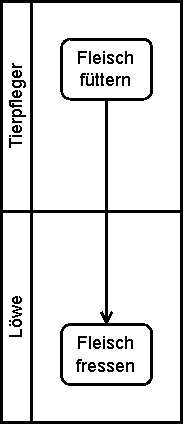
\includegraphics[scale=\sttpFaktor]{Bilder/Kapitel-5/gegenueberstellung_4a.pdf}
				\vspace{\sttpAbstandRand}
			} 
		& 
			\parbox{\sttpHilfB}{\centering
				\vspace{\sttpAbstandRand}
				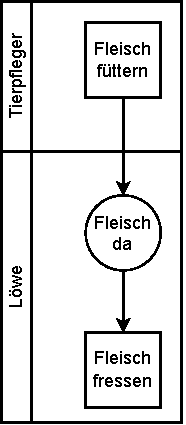
\includegraphics[scale=\sttpFaktor]{Bilder/Kapitel-5/gegenueberstellung_4b.pdf}
				\vspace{\sttpAbstandRand}
			} 
		\\
		
		\hline %-----------------------------
		
			\parbox{\sttpHilfA}{\centering
				Objektknoten \\ / \\ Marken und \\ Kantengewichte} 
		& 
			\parbox{\sttpHilfB}{\centering
				\vspace{\sttpAbstandRand}
				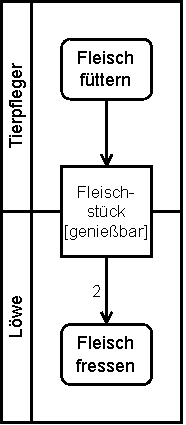
\includegraphics[scale=\sttpFaktor]{Bilder/Kapitel-5/gegenueberstellung_5a.pdf}
				\vspace{\sttpAbstandRand}
			}
		& 
			\parbox{\sttpHilfB}{\centering
				\vspace{\sttpAbstandRand}
				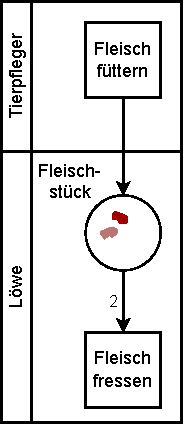
\includegraphics[scale=\sttpFaktor]{Bilder/Kapitel-5/gegenueberstellung_5b.pdf}
				\vspace{\sttpAbstandRand}
			} 
		\\

		\hline %-----------------------------

			\parbox{\sttpHilfA}{\centering
				Anfang \\ und \\ Ende } 
		&  
			\parbox{\sttpHilfB}{\centering
				\vspace{\sttpAbstandRand}
				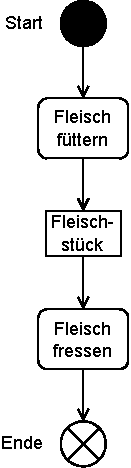
\includegraphics[scale=\sttpFaktor]{Bilder/Kapitel-5/gegenueberstellung_6a.pdf}
				\vspace{\sttpAbstandRand}
			}
		& 
			\parbox{\sttpHilfB}{\centering
				\vspace{\sttpAbstandRand}
				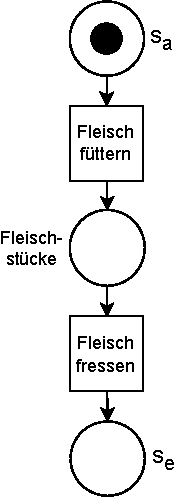
\includegraphics[scale=\sttpFaktor]{Bilder/Kapitel-5/gegenueberstellung_6b.pdf}
				\vspace{\sttpAbstandRand}
			} 
		\\
		
		\hline %-----------------------------
		
			\parbox{\sttpHilfA}{\centering
				Entscheidungs\-knoten} 
		&  
			\parbox{\sttpHilfB}{\centering
				\vspace{\sttpAbstandRand}
				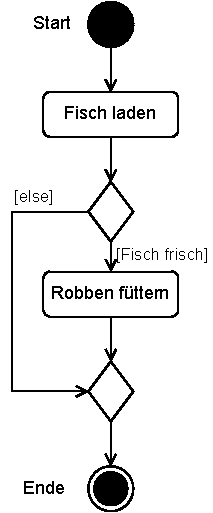
\includegraphics[scale=\sttpFaktor]{Bilder/Kapitel-5/gegenueberstellung_7a.pdf}
				\vspace{\sttpAbstandRand}
			} 
		& 
			\parbox{\sttpHilfB}{\centering
				\vspace{\sttpAbstandRand}
				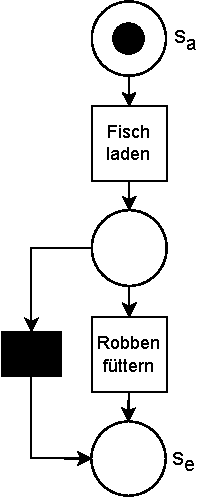
\includegraphics[scale=\sttpFaktor]{Bilder/Kapitel-5/gegenueberstellung_7b.pdf}
				\vspace{\sttpAbstandRand}
			} 
		\\
		
		\hline %-----------------------------
	\end{longtable}
	%	\caption{Gegenüberstellung von Aktivitätsdiagramm- und Petrinetz-Syntax}
	%	\label{fig:gegenueberstellung}
	%\end{figure}

\endgroup


% 5.12
% Kommentierte Literatur beginnt auf neuer Seite
\clearpage
\section{Kommentierte Literatur}

\sttpKommLitItem{Weske}{2024}{Business Process Management}{wes24}{}{}
{Sehr gute Grundlagenliteratur zum Thema Prozessmanagement. \textit{Part II Business Process Modelling} gibt einen Überblick über (Geschäfts-)Prozessmodellierung mit Fokus auf BPMN und Workflow-Management. Auf Englisch.}

\sttpKommLitItem{Aalst}{2016}{Process Mining}{aal16}{}{}
{Einführung in die Themen Data Science und Process Mining. Es werden verschiedene Techniken erläutert, wie aus Daten Prozessmodelle entwickelt werden, aber auch, wie man diese analysieren kann. Auf Englisch.}

\sttpKommLitItem{Reisig}{2010}{Petrinetze}{rei10}{}{}
{Grundlagenliteratur zum Thema Petrinetze in einfacher und gut verständlicher Sprache. Hier wird von High-Level Petrinetzen als allgemeiner Fall ausgegangen -- ein sehr interessanter Ansatz.}

\sttpKommLitItem{Kecher/Salvanos/Hoffmann-Elbern}{2018}{UML~2.5}{kec18}{}{}
{Wie für die UML-Klassendiagramme ist dieses Buch durch seine zahlreichen Lebens\-welt\-beispiele und beispielhaften Programmcodeumsetzungen auch für Zustands-
	\linebreak %%% für Druck
	diagramme, Sequenzdiagramme und Aktivitätsdiagramme gerade für Anfänger der UML eine gute Wahl.}

